% Options for packages loaded elsewhere
\PassOptionsToPackage{unicode}{hyperref}
\PassOptionsToPackage{hyphens}{url}
%
\documentclass[
  12pt,
  oneside]{article}
\usepackage{amsmath,amssymb}
\usepackage{setspace}
\usepackage{iftex}
\ifPDFTeX
  \usepackage[T1]{fontenc}
  \usepackage[utf8]{inputenc}
  \usepackage{textcomp} % provide euro and other symbols
\else % if luatex or xetex
  \usepackage{unicode-math} % this also loads fontspec
  \defaultfontfeatures{Scale=MatchLowercase}
  \defaultfontfeatures[\rmfamily]{Ligatures=TeX,Scale=1}
\fi
\usepackage{lmodern}
\ifPDFTeX\else
  % xetex/luatex font selection
    \setmainfont[]{Times New Roman}
\fi
% Use upquote if available, for straight quotes in verbatim environments
\IfFileExists{upquote.sty}{\usepackage{upquote}}{}
\IfFileExists{microtype.sty}{% use microtype if available
  \usepackage[]{microtype}
  \UseMicrotypeSet[protrusion]{basicmath} % disable protrusion for tt fonts
}{}
\makeatletter
\@ifundefined{KOMAClassName}{% if non-KOMA class
  \IfFileExists{parskip.sty}{%
    \usepackage{parskip}
  }{% else
    \setlength{\parindent}{0pt}
    \setlength{\parskip}{6pt plus 2pt minus 1pt}}
}{% if KOMA class
  \KOMAoptions{parskip=half}}
\makeatother
\usepackage{xcolor}
\usepackage[margin=1in]{geometry}
\usepackage{longtable,booktabs,array}
\usepackage{calc} % for calculating minipage widths
% Correct order of tables after \paragraph or \subparagraph
\usepackage{etoolbox}
\makeatletter
\patchcmd\longtable{\par}{\if@noskipsec\mbox{}\fi\par}{}{}
\makeatother
% Allow footnotes in longtable head/foot
\IfFileExists{footnotehyper.sty}{\usepackage{footnotehyper}}{\usepackage{footnote}}
\makesavenoteenv{longtable}
\usepackage{graphicx}
\makeatletter
\newsavebox\pandoc@box
\newcommand*\pandocbounded[1]{% scales image to fit in text height/width
  \sbox\pandoc@box{#1}%
  \Gscale@div\@tempa{\textheight}{\dimexpr\ht\pandoc@box+\dp\pandoc@box\relax}%
  \Gscale@div\@tempb{\linewidth}{\wd\pandoc@box}%
  \ifdim\@tempb\p@<\@tempa\p@\let\@tempa\@tempb\fi% select the smaller of both
  \ifdim\@tempa\p@<\p@\scalebox{\@tempa}{\usebox\pandoc@box}%
  \else\usebox{\pandoc@box}%
  \fi%
}
% Set default figure placement to htbp
\def\fps@figure{htbp}
\makeatother
\setlength{\emergencystretch}{3em} % prevent overfull lines
\providecommand{\tightlist}{%
  \setlength{\itemsep}{0pt}\setlength{\parskip}{0pt}}
\setcounter{secnumdepth}{5}
% definitions for citeproc citations
\NewDocumentCommand\citeproctext{}{}
\NewDocumentCommand\citeproc{mm}{%
  \begingroup\def\citeproctext{#2}\cite{#1}\endgroup}
\makeatletter
 % allow citations to break across lines
 \let\@cite@ofmt\@firstofone
 % avoid brackets around text for \cite:
 \def\@biblabel#1{}
 \def\@cite#1#2{{#1\if@tempswa , #2\fi}}
\makeatother
\newlength{\cslhangindent}
\setlength{\cslhangindent}{1.5em}
\newlength{\csllabelwidth}
\setlength{\csllabelwidth}{3em}
\newenvironment{CSLReferences}[2] % #1 hanging-indent, #2 entry-spacing
 {\begin{list}{}{%
  \setlength{\itemindent}{0pt}
  \setlength{\leftmargin}{0pt}
  \setlength{\parsep}{0pt}
  % turn on hanging indent if param 1 is 1
  \ifodd #1
   \setlength{\leftmargin}{\cslhangindent}
   \setlength{\itemindent}{-1\cslhangindent}
  \fi
  % set entry spacing
  \setlength{\itemsep}{#2\baselineskip}}}
 {\end{list}}
\usepackage{calc}
\newcommand{\CSLBlock}[1]{\hfill\break\parbox[t]{\linewidth}{\strut\ignorespaces#1\strut}}
\newcommand{\CSLLeftMargin}[1]{\parbox[t]{\csllabelwidth}{\strut#1\strut}}
\newcommand{\CSLRightInline}[1]{\parbox[t]{\linewidth - \csllabelwidth}{\strut#1\strut}}
\newcommand{\CSLIndent}[1]{\hspace{\cslhangindent}#1}

\usepackage{titlesec}
\titleformat{\section}{\normalfont\fontsize{14}{16}\bfseries}{\thesection}{1em}{}
\titleformat{\subsection}{\normalfont\fontsize{13}{15}\bfseries}{\thesubsection}{1em}{}
\titleformat{\subsubsection}{\normalfont\fontsize{12}{14}\bfseries}{\thesubsubsection}{1em}{}
\usepackage{bookmark}
\IfFileExists{xurl.sty}{\usepackage{xurl}}{} % add URL line breaks if available
\urlstyle{same}
\hypersetup{
  hidelinks,
  pdfcreator={LaTeX via pandoc}}

\author{}
\date{\vspace{-2.5em}}

\begin{document}


\begin{titlepage}
    \centering
    
    % University logo (replace with actual path)
    \IfFileExists{ictu-logo.png}{
        
\includegraphics[width=0.5\textwidth]{ictu-logo.png}
    }{
        \vspace*{1cm}
        \textbf{\Large THE ICT UNIVERSITY}
    }
    
    \vspace{1cm}
    
    {\Large Faculty of Information and Communication Technology}
    
    \vspace{1.2cm}
    
    {A dissertation presented and submitted in partial fulfilment of the requirements\\
    for the degree of a Bachelor of Science in Computer Science}
    
    \vspace{0.5cm}

    {Titile}
    
    \textbf{Development of a Skin Lesion Detection and Classification System using Convolutional Neural Networks (CNNs)}
    
    \vspace{0.4cm}
    
    \textbf{By}
    
    \text{Ngane Emmanuel}
    
    \vspace{0.5cm}
    
    {Registration Number: ICTU20222972}
    
    \vspace{1cm}
    
    {Supervised by: Engr. Nkiamboh Tanwi}
    
    \vspace{2cm}
    
    \textbf{\today}
    
    \vfill
\end{titlepage}
\clearpage
\thispagestyle{empty}
\begin{center}
\textbf{\large DECLARATION}
\end{center}

\vspace{1cm}

I declare that the work entitled \textbf{``Development of a Skin Lesion Detection and Classification System using Convolutional Neural Networks (CNNs)''} is my own original work, conceived and presented in the partial fulfilment of the requirement for the degree of a Bachelor of Science in Computer Science at ICT University. This work has not been submitted for any degree or examination in any other university, and that all the sources I have used or quoted have been indicated and acknowledged as complete references.

\vspace{1.2cm}

\begin{tabular}{ll}
Signed \rule{4cm}{0.15mm} \hspace{3cm} & Date: \rule{4cm}{0.15mm} \\ [0.5cm]
Name: \rule{4cm}{0.15mm} & \\ [0.5cm]
Registration Number: \rule{4cm}{0.15mm} & \\
\end{tabular}
\vfill
\clearpage
\thispagestyle{empty}
\begin{center}
\textbf{\large CERTIFICATION}
\end{center}

\vspace{1cm}

This work entitled \textbf{``Development of a Skin Lesion Detection and Classification System using Convolutional Neural Networks (CNNs)''} has been submitted for examination with my approval as the Research Supervisor.

\vspace{2cm}

\begin{tabular}{ll}
Signed \rule{4cm}{0.15mm} \hspace{3cm} & Date: \rule{4cm}{0.15mm} \\ [0.5cm]
Name: \rule{4cm}{0.15mm} & \\
\end{tabular}
\clearpage

\thispagestyle{empty}
\begin{center}
\textbf{\large DEDICATION}
\end{center}

\vspace{2cm} % Adjust spacing as needed

I dedicate this work to my parents, Rev. Dr. Ntoko Samuel Eseh and Mme Ntoko Grace Melioge, and to my loving sister, Ntoko Racheal Edenge, for their unwavering support, encouragement, and sacrifices throughout my academic journey.

\vfill % Pushes the text to the vertical center
\clearpage

\thispagestyle{empty}
\begin{center}
\textbf{\large Acknowledgments}
\end{center}

\vspace{2cm} % Adjust spacing as needed

I would like to express my sincere appreciation to my project supervisor, Engr. Nkiambo Tanwi, whose guidance, feedback, and encouragement were invaluable throughout the course of this project. His expertise and support helped shape both the direction and quality of this research.

I am also grateful to the faculty and staff of the Department of Computer Science, ICT University, for providing the academic foundation and resources necessary for the completion of this work. Their commitment to academic excellence has been instrumental in my development.

Special thanks go to my classmates and friends for their collaboration, feedback, and moral support during the challenging phases of this project. Their insights and motivation helped me stay focused and persistent.

Lastly, I appreciate my family for their continuous encouragement and understanding, which enabled me to dedicate the necessary time and energy to this project.

This project has been a significant learning experience, and I am thankful to all who contributed to its successful completion.

\vfill % Pushes the text to the vertical center
\clearpage

\thispagestyle{empty}
\begin{center}
\textbf{\large FACULTY APPROVAL}
\end{center}

\vspace{1cm}

This dissertation has been duly reviewed by the Department and the Faculty and is ready for examination with our approval.

\vspace{2cm}

\begin{flushright}
\textbf{Approved by}

\vspace{1.5cm}

\begin{tabular}{@{}r@{}}
Signature \hspace{3cm} Date \\ [0.5cm]
\rule{6cm}{0.15mm} \\ [0.2cm]
Engr. Nkiamboh Tanwi \\ [0.3cm]
Supervisor \\[1cm]

Signature \hspace{3cm} Date \\ [0.5cm]
\rule{6cm}{0.15mm} \\ [0.2cm]
Dr. Abdallah Ziraba \\ [0.3cm]
Head of Department \\[1cm]

Signature \hspace{3cm} Date \\ [0.5cm]
\rule{6cm}{0.15mm} \\ [0.2cm]
Dr. Luc Einstein Ngend \\ [0.3cm]
Dean \\
\end{tabular}
\end{flushright}

\vfill
\clearpage

% Abstract Page
\thispagestyle{empty}
\begin{center}
\textbf{\Large ABSTRACT}
\end{center}

\vspace{1cm}

Skin lesions encompass a wide spectrum of conditions, ranging from benign disorders such as eczema, fungal infections, and psoriasis to malignant forms like melanoma and squamous cell carcinoma. Globally, these conditions impose significant public health and economic burdens, with their impact being particularly acute in low-resource regions where specialized dermatological expertise is scarce. In Cameroon and much of sub-Saharan Africa, access to timely and accurate dermatological diagnosis is hindered by limited specialist availability, under-resourced health facilities, and geographic barriers to care. 

This study presents the development of a multi-class skin lesion detection and classification system using Convolutional Neural Networks (CNNs), designed to enhance diagnostic accessibility through automated image analysis. The system was trained on a curated, high-quality dataset compiled from multiple open-access sources, including Kaggle dermatology repositories and the DermNetNZ medical image database. Careful preprocessing and augmentation techniques were employed to normalize image quality, address class imbalance, and improve model robustness across diverse lesion presentations and skin tones.

A fine-tuned ResNet-18 architecture, leveraging transfer learning from the ImageNet dataset, was implemented to classify lesions into multiple diagnostic categories, covering both malignant and non-malignant conditions. The model was trained using supervised learning with categorical cross-entropy loss, and evaluated using metrics including accuracy, precision, recall, and F1-score. The final system achieved a validation accuracy of 75\% and demonstrated consistent performance on the test set, underscoring its potential as a supportive diagnostic aid.

The implementation includes a command-line interface (CLI) for research use and a prototype mobile application framework aimed at offline deployment in rural and underserved settings. By combining computational efficiency with diagnostic breadth, the system offers a cost-effective and scalable approach to skin lesion classification in contexts where traditional healthcare access is limited. 

This project contributes to the growing field of AI-assisted dermatology by emphasizing inclusivity across skin tones and lesion types, while maintaining technical feasibility for low-resource environments. Future improvements will focus on expanding the dataset, integrating explainable AI features, incorporating multi-modal patient data, and validating the system in real-world clinical settings.

\vspace{1cm}
\noindent\textbf{Keywords:} Skin lesion detection, convolutional neural networks, ResNet-18, transfer learning, dataset diversity, mobile health, Cameroon, medical imaging.

\vfill
\clearpage

{
\setcounter{tocdepth}{3}
\tableofcontents
}
\setstretch{1.5}
\newpage

\listoffigures
\newpage

\newpage

\section{Chapter 1: Introduction}\label{chapter-1-introduction}

\subsection{Introduction}\label{introduction}

Skin lesions encompass a broad spectrum of abnormalities in the skin,
ranging from benign conditions such as moles and warts to malignant
manifestations like melanoma and squamous cell carcinoma. Globally,
these dermatological disorders present a significant public health
challenge, with skin cancers alone accounting for millions of new cases
annually and exerting substantial socioeconomic and healthcare burdens
(\citeproc{ref-ogudo2023optimal}{Ogudo et al., 2023}),
(\citeproc{ref-kassem2021machine}{Kassem et al., 2021}). The prevalence
of skin lesions has been amplified by factors such as increased
ultraviolet (UV) exposure due to climate change, demographic
transitions, and lifestyle changes, contributing to both malignant and
non-malignant skin disorders (\citeproc{ref-zafar2023skin}{Zafar et al.,
2023}).

In high-income countries, early diagnosis is often facilitated by access
to trained dermatologists, advanced imaging technologies, and
well-established referral systems. However, in low- and middle-income
countries (LMICs), particularly in sub-Saharan Africa, dermatology
services remain sparse, with a severe shortage of qualified
dermatologists and specialized diagnostic tools
(\citeproc{ref-hay2006skin}{Hay et al., 2006}). This disparity often
leads to delayed diagnoses, inappropriate treatments, and preventable
morbidity and mortality from conditions that are otherwise treatable
when detected early.

Cameroon, like many African nations, faces a dual challenge: the burden
of infectious skin diseases such as fungal infections, scabies, and
bacterial dermatitis coexists with a growing incidence of
non-communicable skin disorders, including actinic keratosis, psoriasis,
and malignant lesions (\citeproc{ref-van2005common}{Hees \& Naafs,
2005}). The limited integration of dermatological screening into primary
healthcare, coupled with the absence of large-scale public awareness
campaigns, exacerbates the problem.

Recent advancements in artificial intelligence (AI) and machine learning
(ML), particularly deep learning-based image analysis, have demonstrated
remarkable potential in automating the detection and classification of
skin lesions with performance levels approaching or surpassing that of
experienced dermatologists (\citeproc{ref-khan2021multi}{Khan et al.,
2021}), (\citeproc{ref-adegun2020fcn}{Adegun \& Viriri, 2020}). Such
systems leverage large annotated datasets to learn discriminative
features directly from dermoscopic or clinical images, enabling fast,
scalable, and cost-effective screening.

This research seeks to harness these technological advancements to
develop a skin lesion detection and classification system capable of
accurately identifying multiple common skin lesion types. The proposed
system integrates a convolutional neural network (CNN) trained on
diverse, high-quality datasets sourced from publicly available
repositories such as Kaggle and curated medical image databases like
DermNetNZ. In addition to the AI model, the system will include a
graphical user interface (GUI) for clinical use, a command-line
interface (CLI) for research purposes, and a mobile application to
extend accessibility to rural and underserved communities. This
comprehensive approach aims to bridge the diagnostic gap, improve early
detection rates, and contribute to the broader objective of reducing the
dermatological disease burden in Cameroon and similar contexts.

\subsection{Background to the Problem}\label{background-to-the-problem}

Dermatological diseases represent one of the most common categories of
health complaints worldwide, with conditions ranging from self-limiting
skin irritations to life-threatening malignancies. The World Health
Organization (WHO) has repeatedly emphasized that skin diseases are
among the top ten causes of non-fatal disease burden globally, and in
certain regions of sub-Saharan Africa, they are among the most frequent
reasons for outpatient consultations (\citeproc{ref-hay2006skin}{Hay et
al., 2006}), (\citeproc{ref-van2005common}{Hees \& Naafs, 2005}). While
conditions like melanoma and basal cell carcinoma dominate skin cancer
statistics in developed nations, the disease landscape in Africa and
particularly Cameroon is more heterogeneous, encompassing a mix of
infectious, inflammatory, and neoplastic disorders.

Traditionally, diagnosis of skin lesions has relied heavily on visual
inspection by a dermatologist, often supplemented by dermoscopic
evaluation or histopathological examination for suspicious cases
(\citeproc{ref-yap2018multimodal}{Yap et al., 2018}). However, this
process is inherently subjective and highly dependent on the clinician's
expertise and experience. In many LMICs, including Cameroon, the ratio
of dermatologists to the population is critically low, often less than
one dermatologist per million inhabitants, leading to substantial
diagnostic delays. Moreover, general practitioners and nurses, who often
serve as first-line healthcare providers, may lack specialized training
in dermatology, further compounding the risk of misdiagnosis or missed
diagnoses.

The advent of AI in medical imaging, particularly the application of
convolutional neural networks (CNNs) to dermoscopic and clinical images,
has opened new possibilities for addressing these challenges
(\citeproc{ref-harangi2018skin}{Harangi, 2018}),
(\citeproc{ref-mahbod2019skin}{Mahbod et al., 2019}). CNNs can
automatically extract hierarchical features from raw image data,
allowing them to differentiate between lesion types with minimal human
intervention. Studies have demonstrated that AI-based diagnostic tools
can achieve diagnostic accuracy comparable to or exceeding that of
experienced dermatologists in controlled settings
(\citeproc{ref-albahar2019skin}{Albahar, 2019}),
(\citeproc{ref-jinnai2020development}{Jinnai et al., 2020}).

Despite these advancements, most existing AI models for skin lesion
classification have been trained and validated on datasets that
predominantly contain images from lighter-skinned populations in Europe,
North America, and Australia (\citeproc{ref-gouda2022detection}{Gouda et
al., 2022}). This raises concerns about model generalizability to
populations with darker skin tones, such as those in sub-Saharan Africa.
Additionally, existing research has often focused on detecting malignant
lesions, particularly melanoma, with limited emphasis on the broader
spectrum of common lesions prevalent in African contexts, such as
eczema, tinea infections, or Kaposi's sarcoma.

This project responds to these gaps by developing a multi-class lesion
classification system specifically curated to include a diverse set of
common skin conditions affecting African populations. The dataset
compilation process involves selecting high-quality images from multiple
Kaggle repositories and supplementing them with clinically verified
images from DermNetNZ, ensuring representation across various lesion
categories and skin tones. Through this approach, the proposed system
aims to offer a clinically relevant, context-sensitive diagnostic
support tool that addresses both the technical challenges of AI
implementation and the pressing healthcare needs of the target
population.

\subsection{Problem Statement}\label{problem-statement}

The early and accurate diagnosis of skin lesions remains a critical
public health challenge in Cameroon and across much of sub-Saharan
Africa. While skin lesions may appear trivial in their initial stages,
certain forms such as malignant melanomas, squamous cell carcinomas, and
basal cell carcinomas, can rapidly progress to life-threatening stages
if left untreated. In parallel, other non-malignant but common
conditions, such as fungal infections, eczema, and psoriasis, can cause
significant discomfort, social stigma, and economic loss due to
chronicity and recurrence.

In many urban centers of high-income countries, advanced diagnostic
services and dermatology specialists are accessible, enabling early
detection and management. However, in Cameroon, the number of
dermatologists is grossly inadequate relative to the population size,
with some regions having no specialist at all
(\citeproc{ref-hay2006skin}{Hay et al., 2006}),
(\citeproc{ref-van2005common}{Hees \& Naafs, 2005}). This shortage
forces patients to rely on general practitioners or traditional healers,
which often leads to delayed diagnoses, mismanagement, or complete
neglect of skin-related health issues.

Furthermore, conventional diagnostic workflows are limited by two key
barriers:\\
1. \textbf{Geographic accessibility} -- Many patients in rural areas
must travel long distances to reach healthcare facilities, resulting in
missed opportunities for early diagnosis.\\
2. \textbf{Resource limitations} -- Even in urban hospitals, dermoscopic
imaging equipment and histopathological services are often scarce or
prohibitively expensive.

Recent developments in artificial intelligence, specifically
convolutional neural networks (CNNs), have shown promise in automating
skin lesion detection and classification with high accuracy
(\citeproc{ref-khan2021multi}{Khan et al., 2021}),
(\citeproc{ref-adegun2020fcn}{Adegun \& Viriri, 2020}). Nonetheless,
most existing models are trained on datasets from lighter-skinned
populations and focus primarily on malignant lesions, limiting their
applicability in African contexts where lesion diversity and skin tone
variations differ significantly (\citeproc{ref-gouda2022detection}{Gouda
et al., 2022}).

The central problem, therefore, is the absence of an accessible,
accurate, and context-specific diagnostic tool for multiple types of
skin lesions prevalent in Cameroon. There is a need for an integrated
system that combines AI-powered lesion detection with user-friendly
interfaces, ranging from clinical desktop applications to mobile apps
that can bridge the diagnostic gap between rural patients, urban
hospitals, and research institutions.

\subsection{Objectives of the Study}\label{objectives-of-the-study}

The overarching aim of this study is to develop a comprehensive skin
lesion detection and classification system that leverages deep learning
techniques to address the diagnostic challenges faced in Cameroon and
similar low-resource settings.

\subsubsection{General Objective}\label{general-objective}

To design and implement an AI-driven system capable of accurately
detecting and classifying multiple types of common skin lesions, with
deployment across desktop, command-line, and mobile platforms to improve
diagnostic accessibility.

\subsubsection{Specific Objectives}\label{specific-objectives}

\begin{enumerate}
    \item To compile and curate a diverse, high-quality dataset of common skin lesion images from multiple open-access sources, including Kaggle repositories and the DermNetNZ medical image database.
    \item To preprocess and augment image data to enhance model robustness..
    \item To train a convolutional neural network (CNN) model optimized for multi-class lesion classification, ensuring high performance on both malignant and non-malignant categories.
    \item To develop a command-line interface (CLI) for research and model testing purposes.
    \item To design and implement a mobile application capable of performing on-device lesion classification for remote and rural healthcare access.
    \item To evaluate the system's performance against standard diagnostic accuracy metrics, including sensitivity, specificity, and overall classification accuracy.
    \item To assess the feasibility of integrating the system into existing telemedicine frameworks in Cameroon.
\end{enumerate}

\subsection{Scope of the Study}\label{scope-of-the-study}

This study focuses on the development of a skin lesion detection and
classification system tailored for the Cameroonian healthcare context,
while incorporating global best practices in AI-assisted dermatological
diagnosis. The scope of the research spans four key dimensions: the
dataset, the technical solution, the deployment platforms, and the
evaluation process.

From a \textbf{data perspective}, the system will be trained and
validated using a carefully curated dataset compiled from multiple
publicly available repositories on Kaggle, supplemented with
high-quality dermatological images sourced from DermNetNZ. These sources
offer a broad spectrum of lesion categories, ranging from malignant
cancers such as melanoma and squamous cell carcinoma to non-malignant
conditions like eczema, psoriasis, and fungal infections. Selection
criteria will prioritize image clarity, correct annotation, diversity of
skin tones, and representation of lesion variations to ensure the
model's applicability across a wide demographic.

From a \textbf{technical perspective}, the system will employ a
convolutional neural network (CNN) architecture fine-tuned for
multi-class classification. Advanced preprocessing techniques, such as
data augmentation and normalization, will be applied to enhance the
model's generalizability across different imaging conditions. While the
primary focus is on image-based diagnosis, the system is not intended to
replace histopathological confirmation, which remains the gold standard
for definitive lesion classification.

From a \textbf{deployment perspective}, the project encompasses three
interfaces:

\begin{enumerate}
\def\labelenumi{\arabic{enumi}.}
\tightlist
\item
  A \textbf{Command-Line Interface (CLI)}, primarily intended for
  researchers and developers for testing and evaluating the AI model.\\
\item
  A \textbf{Mobile Application}, optimized for both offline and online
  usage, to enable healthcare workers and patients in rural areas to
  perform preliminary lesion assessments without constant internet
  connectivity.
\end{enumerate}

From an \textbf{evaluation perspective}, the model will be tested using
standard performance metrics, including accuracy, sensitivity,
specificity, and confusion matrix analysis. The evaluation will
emphasize the system's ability to handle variations in lesion
presentation due to differences in skin pigmentation, image quality, and
environmental lighting.

The project does not aim to cover the entire spectrum of dermatological
conditions, rare or highly complex lesions requiring specialized
diagnostic equipment fall outside the intended operational scope.
Instead, the focus is on delivering a reliable, accessible, and scalable
solution for the most common and clinically significant skin lesions
encountered in Cameroon and similar resource-limited environments.

\subsection{Significance of the Study}\label{significance-of-the-study}

Skin diseases are among the most common health concerns globally, with
billions of people affected each year, spanning all socioeconomic groups
(\citeproc{ref-hay2006skin}{Hay et al., 2006}). In Cameroon and much of
sub-Saharan Africa, the impact of skin lesions is amplified by a
combination of high prevalence, limited specialist care, and widespread
misinformation about skin health. Misdiagnosed or untreated lesions,
whether malignant or non-malignant, can lead to severe health
complications, disfigurement, psychological distress, and in the case of
cancers, increased mortality rates.

The significance of this study lies in its potential to bridge the
diagnostic gap through a context-specific, AI-driven approach. By
leveraging deep learning algorithms and multi-platform deployment, the
system offers a means of providing timely and accurate lesion assessment
to populations that currently lack access to dermatological expertise.
For healthcare providers, this could translate to earlier interventions,
better patient outcomes, and a reduction in the burden on tertiary
healthcare facilities.

From a \textbf{public health perspective}, the project addresses a
critical need in preventive care. Early detection and classification can
significantly reduce treatment costs and improve survival rates in
malignant cases, while minimizing chronic complications in non-malignant
cases. Moreover, the system's mobile deployment makes it a practical
tool for community health workers conducting outreach in rural and
peri-urban areas.

From a \textbf{technological perspective}, the research contributes to
the growing field of AI in medical imaging by demonstrating how existing
machine learning methods can be adapted to underrepresented populations.
Many existing AI models for skin lesion classification are trained
predominantly on lighter-skinned datasets, making them less effective
for darker skin tones (\citeproc{ref-gouda2022detection}{Gouda et al.,
2022}). By incorporating diverse skin tone representation from datasets
like DermNetNZ and Kaggle repositories, this study advances the
inclusivity and fairness of medical AI systems.

From an \textbf{academic perspective}, the project provides a valuable
reference for future studies in both computer vision and health
informatics within the African context. The integration of a
research-oriented CLI, a mobile health application, and a clinical GUI
sets a precedent for multi-platform medical AI systems designed for
low-resource settings.

Ultimately, the study seeks to contribute toward Sustainable Development
Goal 3 (Good Health and Well-being) by enabling accessible, affordable,
and high-quality dermatological diagnostics in regions where such
services are currently limited or absent.

\subsubsection{1.7 Limitations of the
Study}\label{limitations-of-the-study}

While this study seeks to develop a comprehensive, AI-powered skin
lesion detection and classification system, several constraints
inevitably shape the scope and potential impact of the research. First,
the dataset, although carefully curated from high-quality open-access
sources such as Kaggle repositories and the DermNetNZ medical image
database, may not capture the full diversity of skin lesion
presentations across all ethnic groups and age categories. This
limitation is particularly relevant for sub-Saharan African populations,
where variations in skin pigmentation can influence lesion visibility
and morphology, potentially impacting model generalization
(\citeproc{ref-hay2006skin}{Hay et al., 2006}),
(\citeproc{ref-van2005common}{Hees \& Naafs, 2005}).

Second, although image preprocessing and augmentation techniques are
employed to mitigate overfitting and improve robustness, the absence of
histopathological confirmation for all dataset images introduces an
inherent diagnostic uncertainty. Clinical image-based diagnosis, while
valuable, cannot entirely substitute for biopsy-confirmed ground truth,
especially in differentiating visually similar lesion types
(\citeproc{ref-zafar2023skin}{Zafar et al., 2023}).

Third, computational resource limitations constrain the complexity and
scale of model experimentation. While transfer learning with established
CNN architectures, such as ResNet, offers strong baseline performance,
exploring more computationally intensive models or ensemble methods may
be restricted due to hardware constraints. This also impacts the breadth
of hyperparameter optimization that can be conducted within the project
timeline.

Fourth, the current implementation focuses primarily on classification
accuracy and does not yet incorporate a complete clinical decision
support framework, such as integration with electronic health records
(EHRs) or automated referral systems. Similarly, the system's deployment
is confined to a mobile application and a research-oriented command-line
interface, without the immediate inclusion of a graphical interface for
clinical integration, an enhancement reserved for future development
phases.

Finally, while the study includes performance evaluation using standard
diagnostic metrics (e.g., sensitivity, specificity, overall accuracy),
real-world clinical validation with dermatologists or in live
telemedicine settings is beyond the scope of the present work. This
limits immediate translation into routine healthcare workflows but
provides a foundation for subsequent validation studies.

\subsubsection{1.8 Organization of the
Study}\label{organization-of-the-study}

The remainder of this thesis is organized into five chapters, each
systematically addressing a core component of the research.

\begin{itemize}
\tightlist
\item
  \textbf{Chapter 1 -- Introduction}: Provides an overview of the
  research problem, contextual background, study objectives, scope,
  significance, and limitations, setting the stage for the
  investigation.
\item
  \textbf{Chapter 2 -- Literature Review}: Presents a comprehensive
  examination of existing studies on skin lesion detection and
  classification, machine learning and deep learning techniques applied
  to medical imaging, and relevant mobile health (mHealth) application
  frameworks. This chapter critically evaluates the strengths and
  weaknesses of prior approaches, identifying gaps that this study seeks
  to address.
\item
  \textbf{Chapter 3 -- Methodology}: Describes the research design,
  dataset collection and curation process, preprocessing and
  augmentation strategies, CNN architecture selection, training
  procedures, and performance evaluation metrics. It also outlines the
  mobile application and CLI implementation details.
\item
  \textbf{Chapter 4 -- Results and Discussion}: Reports and analyzes
  experimental results, including classification performance, error
  analysis, and comparative evaluation against existing methods. The
  discussion interprets these findings in the context of the study
  objectives and broader literature.
\item
  \textbf{Chapter 5 -- Conclusion and Future Work}: Summarizes key
  findings, reiterates the contributions of the study, and outlines
  limitations alongside recommended directions for future research,
  including potential clinical integration and large-scale deployment
  strategies.
\end{itemize}

This structured organization ensures a logical progression from problem
identification through methodological implementation to empirical
validation and future considerations, facilitating clarity and coherence
for both technical and non-technical readers.

\newpage

\section{Chapter 2: Literature
Review}\label{chapter-2-literature-review}

\subsection{Introduction}\label{introduction-1}

The human skin, as the largest organ of the body, serves as the first
line of defense against environmental insults, pathogens, and physical
trauma. It performs essential physiological roles including
thermoregulation, sensory perception, and immunological protection.
However, the skin is susceptible to a wide range of pathological
conditions, collectively referred to as skin lesions, which can
significantly impair an individual's quality of life and, in severe
cases, become life-threatening (\citeproc{ref-hay2006skin}{Hay et al.,
2006}). These lesions may arise from infectious agents, autoimmune
disorders, genetic anomalies, or prolonged environmental exposure, with
their clinical presentation varying from benign and self-limiting forms
to aggressive malignancies (\citeproc{ref-van2005common}{Hees \& Naafs,
2005}).

Globally, skin diseases constitute a substantial public health
challenge, ranking among the top causes of non-fatal disease burden.
According to the Global Burden of Disease Study, conditions such as
eczema, acne, and fungal infections collectively affect billions of
individuals worldwide, while skin cancers contribute significantly to
morbidity and mortality in certain regions
(\citeproc{ref-zafar2023skin}{Zafar et al., 2023}). In sub-Saharan
Africa, and specifically in Cameroon, the prevalence of skin lesions is
amplified by climatic factors such as high ultraviolet (UV) index,
tropical humidity, and widespread infectious disease exposure, combined
with limited access to dermatological specialists and diagnostic
facilities (\citeproc{ref-hay2006skin}{Hay et al., 2006}). Rural
communities often face the most acute challenges, where early detection
and treatment are hindered by geographical, infrastructural, and
socioeconomic constraints.

Recent advances in Artificial Intelligence (AI), particularly in
computer vision, have opened promising avenues for automated skin lesion
analysis. Machine learning and deep learning techniques, particularly
Convolutional Neural Networks (CNNs), have demonstrated superior
performance in differentiating between lesion types, sometimes rivalling
trained dermatologists in diagnostic accuracy
(\citeproc{ref-kassem2021machine}{Kassem et al., 2021}),
(\citeproc{ref-ogudo2023optimal}{Ogudo et al., 2023}). Leveraging such
tools in low-resource settings could significantly enhance early
diagnosis, improve treatment outcomes, and reduce the long-term health
and economic burdens associated with skin diseases.

This chapter reviews the existing literature on skin lesion types, their
epidemiology, and the role of AI in dermatological diagnostics, with
particular emphasis on the African context. It also outlines the
technical underpinnings of CNN-based approaches, dataset challenges, and
existing AI-enabled systems for skin lesion detection.

\subsection{Overview of Skin Lesions and Skin
Cancer}\label{overview-of-skin-lesions-and-skin-cancer}

Skin lesions represent a broad spectrum of structural or functional
abnormalities affecting the skin's epidermal, dermal, or subcutaneous
layers. They are typically classified according to their clinical
appearance, etiology, and pathological significance, ranging from
benign, non-cancerous conditions to malignant cancers that pose
significant health risks (\citeproc{ref-zafar2023skin}{Zafar et al.,
2023}). Understanding the characteristics, prevalence, and diagnostic
challenges associated with each category is crucial for designing
AI-assisted diagnostic systems capable of reliable, multi-class
classification across diverse lesion types.

\subsubsection{Non-Cancerous Lesions}\label{non-cancerous-lesions}

Non-cancerous lesions comprise the majority of dermatological cases
encountered in both primary and specialized care. These include
inflammatory conditions such as eczema and psoriasis, infectious
diseases like fungal infections and bacterial dermatoses, pigmentary
disorders such as vitiligo, and benign growths including seborrheic
keratoses and skin tags (\citeproc{ref-hay2006skin}{Hay et al., 2006}).
While these lesions are typically non-fatal, they can cause chronic
discomfort, psychological distress, and social stigma, especially when
affecting visible body areas.

In Africa, the high prevalence of infectious dermatoses is closely
linked to environmental and socioeconomic conditions. Fungal infections
such as tinea capitis are particularly common among children in rural
and peri-urban areas due to overcrowding, limited hygiene facilities,
and humid climatic conditions (\citeproc{ref-van2005common}{Hees \&
Naafs, 2005}). Similarly, bacterial skin infections like impetigo and
cellulitis are widespread, often arising as secondary infections in
individuals with compromised skin barriers from insect bites, eczema, or
other dermatological conditions.

Chronic inflammatory diseases such as eczema and psoriasis, though less
prevalent than infectious dermatoses, represent a significant health
burden due to their recurrent nature and the need for long-term
management. In many low-resource settings, limited access to
dermatologists and diagnostic tools leads to misdiagnosis, inappropriate
treatment, and poor disease control. Pigmentary disorders such as
vitiligo and post-inflammatory hyperpigmentation are also of particular
concern in African populations, where cultural perceptions and stigma
may influence healthcare-seeking behavior
(\citeproc{ref-hay2006skin}{Hay et al., 2006}).

From a diagnostic perspective, the visual similarity between
non-cancerous and cancerous lesions can pose a challenge, particularly
for general practitioners without specialized dermatological training.
AI-driven image analysis tools have the potential to assist in
differentiating these lesions, improving diagnostic accuracy in settings
where specialist input is scarce.

\subsubsection{Cancerous Lesions}\label{cancerous-lesions}

Cancerous lesions, though less common than non-cancerous forms, are of
critical concern due to their potential for metastasis and mortality.
The most prevalent malignant skin cancers include melanoma, squamous
cell carcinoma (SCC), and basal cell carcinoma (BCC). While melanoma is
less frequent in darker skin tones, its prognosis is often poorer in
African populations due to late-stage diagnosis
(\citeproc{ref-zafar2023skin}{Zafar et al., 2023}). SCC and BCC, on the
other hand, may occur in sun-exposed or chronically damaged skin
regardless of skin tone.

Globally, skin cancers represent a significant proportion of all cancer
diagnoses, with an estimated 1.5 million new cases annually
(\citeproc{ref-kassem2021machine}{Kassem et al., 2021}). In high-income
countries, public health campaigns and widespread access to
dermatological care have improved early detection rates, leading to
better survival outcomes. In contrast, in many African countries,
including Cameroon, public awareness of skin cancer remains low, and
access to diagnostic biopsies and histopathology services is limited.
Consequently, patients often present with advanced disease stages,
reducing treatment options and survival prospects.

Risk factors for skin cancer in African populations include albinism,
chronic scarring from burns or ulcers, prolonged exposure to UV
radiation (especially among outdoor workers), and certain viral
infections such as human papillomavirus (HPV). Individuals with
albinism, in particular, face a dramatically elevated risk of developing
SCC due to the absence of protective melanin in the skin.

Diagnosing skin cancer in low-resource settings is challenging due to
both infrastructural and human resource constraints. Dermoscopy,
histopathology, and other confirmatory diagnostic modalities may be
unavailable outside urban tertiary hospitals. In such contexts, mobile
AI-assisted diagnostic tools can play an instrumental role in triaging
suspicious lesions, guiding referrals, and facilitating earlier
intervention.

\subsection{Role of Artificial Intelligence in
Dermatology}\label{role-of-artificial-intelligence-in-dermatology}

Artificial Intelligence (AI) has emerged as a transformative force in
medical diagnostics, with dermatology standing out as a field
particularly well-suited to AI-driven interventions. This suitability
stems from the inherently visual nature of dermatological assessment,
where clinical diagnosis often relies heavily on visual inspection of
lesion morphology, color, texture, and distribution patterns. AI
systems, especially those based on computer vision, can replicate and,
in some cases, surpass human pattern recognition capabilities by
analyzing large volumes of annotated images
(\citeproc{ref-kassem2021machine}{Kassem et al., 2021}),
(\citeproc{ref-ogudo2023optimal}{Ogudo et al., 2023}).

In recent years, deep learning algorithms have demonstrated diagnostic
performance comparable to, and occasionally exceeding, that of
board-certified dermatologists
(\citeproc{ref-esteva2017dermatologist}{Esteva et al., 2017}). These
advancements have been facilitated by the availability of large-scale
annotated image datasets, improvements in computational power, and
algorithmic innovations in neural network architectures. AI-powered
systems have been successfully developed to identify and differentiate
between multiple skin lesion types, including both malignant and
non-malignant conditions, with high sensitivity and specificity.

Beyond diagnostic accuracy, AI offers significant advantages in
scalability and accessibility. Once trained, AI models can be deployed
on a wide range of devices from high-performance clinical workstations
to mobile smartphones, making them particularly valuable in low-resource
environments. In rural areas of Cameroon, for example, where access to
dermatologists is limited, AI-powered mobile applications could enable
preliminary screening and triage, directing patients with suspicious
lesions to specialized care.

Another important role of AI in dermatology lies in \textbf{decision
support}. AI systems can assist clinicians by highlighting regions of
interest, providing probability scores for different lesion classes, and
integrating clinical metadata (such as patient age, lesion history, and
risk factors) into predictive models. This reduces the likelihood of
oversight in busy clinical environments and supports more consistent
diagnostic outcomes.

Furthermore, AI-based lesion analysis is not limited to classification.
Emerging research is exploring its application in lesion segmentation,
disease progression tracking, and even predictive analytics for
treatment response. Such capabilities could support not only individual
patient management but also large-scale epidemiological surveillance.

Despite these strengths, AI adoption in dermatology is not without
challenges. Issues such as dataset bias, lack of diverse representation
(especially for darker skin tones), and limited interpretability of deep
learning models can affect trust and clinical uptake
(\citeproc{ref-gouda2022detection}{Gouda et al., 2022}). Ethical and
regulatory considerations ranging from patient data privacy to liability
in the event of misdiagnosis, also remain critical hurdles. Addressing
these concerns will be essential for ensuring that AI complements rather
than replaces clinical judgment, particularly in sensitive medical
contexts.

\subsection{Convolutional Neural Networks
(CNNs)}\label{convolutional-neural-networks-cnns}

Convolutional Neural Networks (CNNs) represent the cornerstone of modern
computer vision and have become the dominant architecture for image
classification tasks, including dermatological image analysis. Inspired
by the organization of the animal visual cortex, CNNs are designed to
automatically learn hierarchical feature representations directly from
raw pixel data, eliminating the need for manual feature engineering
(\citeproc{ref-lecun2015deep}{LeCun et al., 2015}).

A typical CNN architecture comprises several key components:

\begin{enumerate}
\def\labelenumi{\arabic{enumi}.}
\item
  \textbf{Convolutional Layers} -- These layers apply a series of
  learnable filters to the input image, producing feature maps that
  capture spatial hierarchies such as edges, textures, and shapes. Early
  layers detect simple patterns, while deeper layers learn more complex
  and abstract features relevant to classification.
\item
  \textbf{Pooling Layers} -- Pooling operations (e.g., max pooling,
  average pooling) reduce the spatial dimensions of feature maps,
  thereby decreasing computational load and controlling overfitting
  while retaining the most salient information.
\item
  \textbf{Activation Functions} -- Non-linear activation functions, such
  as ReLU (Rectified Linear Unit), introduce non-linearity into the
  network, enabling it to learn complex decision boundaries.
\item
  \textbf{Fully Connected Layers} -- These layers interpret the
  high-level features extracted by convolutional and pooling layers,
  ultimately producing class probability scores through a softmax or
  sigmoid activation function.
\end{enumerate}

The strength of CNNs in dermatology lies in their ability to extract
discriminative features from lesion images, even in the presence of
significant variability in lesion size, shape, color, and background
noise. This is particularly important for differentiating between
lesions with subtle morphological differences, such as differentiating
an atypical mole from early-stage melanoma.

In the context of skin lesion classification, CNNs have been
successfully applied to both binary classification tasks (e.g., benign
vs malignant) and multi-class classification covering a range of lesion
types (\citeproc{ref-kassem2021machine}{Kassem et al., 2021}). Their
performance is further enhanced through techniques such as \textbf{data
augmentation} (rotations, flips, scaling, color jittering) and
\textbf{regularization} (dropout, weight decay), which improve
generalization and robustness.

However, training CNNs from scratch requires large, balanced datasets,
an obstacle in medical imaging where data is often scarce and unevenly
distributed across classes. This limitation has driven widespread
adoption of \textbf{transfer learning}, wherein CNN architectures
pre-trained on large general-purpose datasets (such as ImageNet) are
fine-tuned on specific medical datasets. Models like ResNet, Inception,
and EfficientNet have been extensively leveraged in this manner,
yielding strong results even with limited medical image data.

For this project, CNNs form the foundational architecture of the lesion
detection and classification system, enabling automated feature
extraction and classification in a manner that is both scalable and
adaptable to diverse deployment environments. Their proven success in
similar tasks makes them a natural choice for addressing the diagnostic
challenges associated with skin lesions in Cameroon and other
low-resource settings.

\subsection{Transfer Learning and ResNet
Models}\label{transfer-learning-and-resnet-models}

Training deep learning models from scratch typically requires vast
datasets containing millions of annotated images. In medical imaging,
however, such large-scale datasets are rare due to privacy concerns, the
cost of expert annotations, and the limited prevalence of certain
conditions (\citeproc{ref-gouda2022detection}{Gouda et al., 2022}). This
scarcity makes \textbf{transfer learning} a practical and effective
approach for developing high-performing models with limited
domain-specific data.

Transfer learning involves leveraging a model pre-trained on a large,
general-purpose dataset such as ImageNet, which contains over 14 million
images across 1,000 classes and adapting it to a new but related task
(\citeproc{ref-lecun2015deep}{LeCun et al., 2015}). In this paradigm,
the lower layers of the pre-trained model, which capture generic
features like edges, textures, and shapes, are retained, while the
higher layers, which learn task-specific features, are fine-tuned on the
target medical dataset. This approach reduces training time, lowers
computational requirements, and mitigates the risk of overfitting.

Among the various architectures used for transfer learning,
\textbf{Residual Networks (ResNet)} have become particularly prominent
due to their ability to train very deep networks without succumbing to
the vanishing gradient problem (\citeproc{ref-he2016deep}{He et al.,
2016}). ResNet's innovation lies in its \emph{residual blocks}, which
introduce shortcut connections that allow gradients to flow more easily
through the network during backpropagation. This architecture enables
the training of models with hundreds of layers while maintaining
stability and accuracy.

ResNet-18, ResNet-34, and ResNet-50 are among the most widely used
variants in medical imaging applications, each offering a trade-off
between computational complexity and representational power. For skin
lesion classification, ResNet architectures have consistently
demonstrated strong performance, particularly when fine-tuned with
domain-specific data and augmented through preprocessing techniques such
as rotation, scaling, and color normalization
(\citeproc{ref-kassem2021machine}{Kassem et al., 2021}).

In the context of this study, ResNet-18 was selected for its balance
between accuracy and computational efficiency, making it suitable for
deployment on both research environments and resource-constrained
devices like smartphones. Transfer learning with ResNet-18 allows the
model to benefit from robust, pre-learned visual features while adapting
to the nuances of dermatological imagery from diverse sources, including
those representing darker skin tones and non-cancerous lesions that are
often underrepresented in global datasets.

\subsection{Dataset Challenges in Medical
Imaging}\label{dataset-challenges-in-medical-imaging}

The success of AI systems in medical imaging is intrinsically tied to
the quality, diversity, and representativeness of the datasets used for
training and evaluation. In dermatology, this presents several
significant challenges.

\textbf{1. Data Scarcity and Class Imbalance} -- High-quality, annotated
dermatological datasets are limited, particularly for rare conditions
and underrepresented demographics. Publicly available datasets such as
those on Kaggle or DermNetNZ often contain disproportionate numbers of
images for certain lesion types, leading to class imbalance. Models
trained on such datasets risk becoming biased toward majority classes,
resulting in reduced accuracy for minority categories
(\citeproc{ref-gouda2022detection}{Gouda et al., 2022}).

\textbf{2. Limited Skin Tone Representation} -- Many benchmark datasets
are heavily skewed toward lighter skin tones, reflecting their origins
in high-income, predominantly Caucasian populations
(\citeproc{ref-gouda2022detection}{Gouda et al., 2022}). This lack of
diversity can lead to systematic biases, where models perform well on
lighter skin but poorly on darker tones---a critical limitation when
deploying AI tools in African contexts.

\textbf{3. Variability in Image Acquisition} -- Images in dermatology
can be captured under a wide range of conditions, including variations
in lighting, background, focus, and resolution. Differences in equipment
from professional dermatoscopes to smartphone cameras, introduce further
heterogeneity, making model generalization more difficult
(\citeproc{ref-zafar2023skin}{Zafar et al., 2023}). Robust preprocessing
pipelines, including color correction, normalization, and augmentation,
are essential to mitigate these effects.

\textbf{4. Annotation Quality and Consistency} -- Accurate labeling of
lesion types often requires expert dermatological input. In public
datasets, annotations may be inconsistent or based solely on visual
inspection rather than biopsy-confirmed diagnoses. This introduces noise
into the training data, potentially lowering model performance
(\citeproc{ref-van2005common}{Hees \& Naafs, 2005}).

\textbf{5. Ethical and Privacy Concerns} -- Medical image datasets must
comply with strict privacy regulations to protect patient identities.
This can limit the sharing of comprehensive datasets, particularly those
including metadata such as patient age, sex, and medical history.
De-identification processes, while necessary, may also remove
potentially valuable contextual information.

For this project, these challenges were addressed through
\textbf{multi-source dataset compilation}, selecting high-quality images
from multiple Kaggle repositories and the DermNetNZ image database.
Images were chosen based on clarity, annotation reliability, and
diversity in lesion presentation. Preprocessing steps, including
augmentation techniques, were applied to improve model robustness. While
this approach does not entirely eliminate dataset-related limitations,
it provides a strong foundation for training a model capable of handling
real-world variability in skin lesion imagery.

\subsubsection{Review of Existing
Systems}\label{review-of-existing-systems}

The development of automated skin lesion detection systems has evolved
significantly over the past three decades, transitioning from rule-based
image processing algorithms to advanced deep learning frameworks capable
of multi-class classification. Early computer-aided diagnosis (CAD)
systems, developed in the late 1990s and early 2000s, primarily relied
on handcrafted features such as color histograms, shape descriptors, and
texture measures, combined with classical classifiers like Support
Vector Machines (SVMs) and k-Nearest Neighbors (k-NN). While these
systems achieved moderate success in controlled environments, their
reliance on manually engineered features made them highly sensitive to
variations in lighting, resolution, and lesion morphology
(\citeproc{ref-gouda2022detection}{Gouda et al., 2022}).

Over the past decade, deep learning, particularly Convolutional Neural
Networks (CNNs) has revolutionized dermatological image analysis.
CNN-based models eliminate the need for manual feature extraction by
learning hierarchical feature representations directly from pixel data
(\citeproc{ref-lecun2015deep}{LeCun et al., 2015}). Notable milestones
include the work of Esteva et al., who demonstrated dermatologist-level
classification of skin cancer using a CNN trained on over 129,000
clinical images (\citeproc{ref-esteva2017dermatologist}{Esteva et al.,
2017}), and the introduction of transfer learning approaches that
significantly reduce the data requirements for effective model training
(\citeproc{ref-he2016deep}{He et al., 2016}).

Several prominent publicly available systems illustrate the current
state of the art. For example, the \textbf{ISIC (International Skin
Imaging Collaboration)} challenge platforms have driven substantial
progress by providing standardized datasets and benchmarking
opportunities for skin lesion classification and segmentation tasks.
Solutions from top-performing teams often integrate deep CNN
architectures such as ResNet, Inception, and EfficientNet, combined with
ensemble learning and advanced data augmentation techniques.

In commercial and practical deployment contexts, mobile applications
such as \emph{SkinVision} and \emph{Miiskin} leverage AI to provide
lesion risk assessments directly to users via smartphone cameras. While
these tools have expanded public access to preliminary screening, they
often focus on binary classification (e.g., suspicious
vs.~non-suspicious) and may not comprehensively cover the range of
benign and malignant lesion types relevant in diverse populations,
particularly in low-resource settings like Cameroon.

Within academic research, several studies have explored multi-class
lesion classification. Kassem et al.~proposed a CNN-based framework
achieving high accuracy across seven lesion classes in the HAM10000
dataset (\citeproc{ref-kassem2021machine}{Kassem et al., 2021}), while
Ogudo et al.~adapted a transfer learning approach for African skin
tones, underscoring the importance of dataset diversity
(\citeproc{ref-ogudo2023optimal}{Ogudo et al., 2023}). These studies
highlight the growing focus on inclusivity and generalizability in AI
dermatology systems.

Despite these advancements, limitations persist. Many existing systems
are trained on datasets that lack representation of darker skin tones,
have a narrow lesion type coverage, or fail to address deployment
constraints such as offline functionality and low computational
resources. Furthermore, while commercial solutions often reach end-users
quickly, they may not undergo the same level of clinical validation or
peer-reviewed scrutiny as academic research outputs.

\subsection{Research Gap}\label{research-gap}

While the progress in AI-powered dermatological diagnostics over the
last decade has been remarkable, several gaps remain, particularly in
the context of African healthcare systems.

\textbf{1. Dataset Representation} -- Most high-performing models are
trained on datasets dominated by images from lighter skin tones. This
limits their diagnostic accuracy when applied to African populations,
where lesion appearance can differ significantly due to higher melanin
content and unique environmental exposure patterns
(\citeproc{ref-gouda2022detection}{Gouda et al., 2022}). The lack of
comprehensive datasets covering both malignant and non-malignant lesions
in darker skin is a critical barrier.

\textbf{2. Multi-Class Coverage} -- Many commercial and academic systems
prioritize melanoma detection due to its high mortality rate in
fair-skinned populations. However, in African contexts, non-cancerous
lesions, such as fungal infections, eczema, and pigmentary disorders,
constitute the majority of dermatological cases and therefore require
equal diagnostic attention.

\textbf{3. Deployment in Low-Resource Settings} -- Existing systems
often assume reliable internet connectivity and high-performance
computing infrastructure, making them unsuitable for rural or
underserved regions. Offline-capable, computationally efficient models
are needed to bridge this gap.

\textbf{4. Clinical Integration and Trust} -- Limited collaboration
between AI developers and healthcare providers in Africa has slowed the
integration of AI tools into clinical workflows. Moreover, clinicians
may be hesitant to adopt AI systems without clear interpretability,
validation on local datasets, and regulatory approval.

\textbf{5. Comprehensive Diagnostic Workflow} -- While classification
accuracy is a major focus of existing research, other aspects of the
diagnostic process such as lesion segmentation, tracking over time, and
integration with patient health records, remain underexplored in
resource-constrained contexts.

This study addresses these gaps by developing a \textbf{multi-class skin
lesion classification system} optimized for deployment in Cameroon. The
approach combines a curated dataset from multiple open-access sources
(Kaggle repositories and DermNetNZ), robust preprocessing and
augmentation, transfer learning using ResNet-18, and deployment pathways
that accommodate both research and mobile application environments. By
doing so, it aims to improve diagnostic accuracy across a broader range
of lesions, enhance representation for darker skin tones, and enable
accessibility in low-resource healthcare settings.

\subsection{Summary}\label{summary}

This chapter has provided a comprehensive review of the literature
relevant to the development of AI-powered skin lesion detection and
classification systems. The discussion began with an overview of skin
lesions, distinguishing between non-cancerous and cancerous categories,
and emphasizing their prevalence and diagnostic challenges both globally
and within the African context. The role of AI in dermatology was
examined, with a particular focus on CNN architectures, transfer
learning strategies, and the ResNet model family, which has proven
highly effective in medical imaging tasks.

Dataset challenges in medical imaging were explored in detail,
highlighting issues such as class imbalance, limited representation of
darker skin tones, variability in image acquisition, and annotation
quality. The review of existing systems illustrated the evolution of
lesion detection technologies from early handcrafted-feature approaches
to modern deep learning-based solutions, while also identifying their
limitations in terms of inclusivity, deployment feasibility, and
comprehensive lesion coverage.

Finally, the research gap analysis underscored the need for multi-class,
skin-tone-inclusive, resource-efficient diagnostic systems that can be
deployed effectively in low-resource settings such as Cameroon. The
following chapter will present the methodology adopted for this study,
detailing the dataset compilation, preprocessing, model training,
evaluation, and deployment strategies used to develop the proposed skin
lesion classification system.

\newpage

\section{Chapter 3: Methodology}\label{chapter-3-methodology}

\subsection{Introduction}\label{introduction-2}

The methodology adopted for this research project provides a systematic
framework for developing, training, and evaluating a skin lesion
detection and classification system. The primary objective of the
methodology is to ensure that each stage of the project, from data
acquisition to model deployment is structured, reproducible, and
grounded in established machine learning best practices. The complexity
of dermatological image analysis, combined with the variability of skin
lesion types, demands a rigorous approach to both data handling and
algorithmic design. In this study, the methodology not only addresses
the technical aspects of convolutional neural network (CNN)
implementation but also incorporates considerations for application
development, user interaction, and deployment.

Skin lesion classification presents unique challenges. Unlike standard
image classification tasks, dermatological images often exhibit high
intra-class variability and subtle inter-class differences. Conditions
such as \textbf{melanoma} and \textbf{nevus} can appear visually similar
under certain imaging conditions, while diseases like
\textbf{chickenpox}, \textbf{measles}, and \textbf{monkeypox} may share
overlapping lesion morphologies. This complexity is further compounded
by variations in image acquisition methods, lighting conditions, skin
tones, and anatomical locations. A robust methodology must therefore be
capable of addressing these challenges through appropriate data
preprocessing, feature extraction, and model optimization techniques.

The development of this system follows a structured lifecycle that draws
upon the \textbf{CRoss Industry Standard Process for Data Mining
(CRISP-DM)} methodology, widely recognized for its flexibility and
applicability to data science projects. The CRISP-DM model consists of
six iterative phases: \textbf{Business Understanding}, \textbf{Data
Understanding}, \textbf{Data Preparation}, \textbf{Modeling},
\textbf{Evaluation}, and \textbf{Deployment}, each of which is adapted
to the specific context of this project. This structure facilitates not
only the creation of a high-performing CNN-based classifier but also
ensures that the final product can be integrated into practical
diagnostic workflows through both a Command-Line Interface (CLI) and a
mobile application.

A key differentiator of this project, compared to many prior works
(\citeproc{ref-khan2021multi}{Khan et al., 2021};
\citeproc{ref-ogudo2023optimal}{Ogudo et al., 2023};
\citeproc{ref-zafar2023skin}{Zafar et al., 2023}), is the scope of the
dataset. While datasets such as HAM10000 primarily focus on malignant
and benign skin tumors, the dataset in this study encompasses a broader
range of dermatological conditions, including viral, bacterial, fungal,
autoimmune, and parasitic skin diseases. This comprehensive dataset,
covering \textbf{33 distinct categories} such as \textbf{Acne},
\textbf{Actinic Keratosis}, \textbf{Ringworm}, \textbf{Leprosy},
\textbf{Basal Cell Carcinoma}, and \textbf{Vitiligo}, allows for a more
inclusive diagnostic support system capable of handling diverse clinical
scenarios.

The methodology outlined in this chapter provides the foundation for:

\begin{itemize}
\tightlist
\item
  Efficient preprocessing and augmentation techniques to enhance dataset
  diversity.
\item
  Fine-tuning of a \textbf{ResNet-18} architecture pre-trained on
  ImageNet to adapt to the specific features of dermatological imagery.
\item
  Training strategies incorporating \textbf{class weighting},
  \textbf{early stopping}, and \textbf{learning rate scheduling} to
  improve generalization and avoid overfitting.
\item
  Evaluation protocols employing multiple performance metrics, including
  \textbf{accuracy}, \textbf{precision}, \textbf{recall}, and
  \textbf{F1-score}.
\item
  Integration of the trained model into an accessible and user-friendly
  application environment.
\end{itemize}

Ultimately, the methodological approach ensures that the system is both
technically sound and practically relevant, with the potential for
deployment in clinical and teledermatology contexts.

\subsection{Project Framework and
Approach}\label{project-framework-and-approach}

The \textbf{CRoss Industry Standard Process for Data Mining (CRISP-DM)}
methodology serves as the guiding framework for the development of the
skin lesion detection and classification system. Originally designed for
data mining projects, CRISP-DM has been widely adapted in the field of
machine learning and artificial intelligence due to its structured yet
flexible nature (\citeproc{ref-ruparelia2010software}{Ruparelia, 2010};
\citeproc{ref-shafiq2021literature}{Shafiq et al., 2021}). The six
phases of CRISP-DM, \textbf{Business Understanding}, \textbf{Data
Understanding}, \textbf{Data Preparation}, \textbf{Modeling},
\textbf{Evaluation}, and \textbf{Deployment}, are not strictly linear
but rather iterative, allowing for feedback loops and refinements at any
stage.

\subsubsection{Business Understanding}\label{business-understanding}

The primary goal of this project is to develop an automated skin lesion
classification system that can aid healthcare professionals and patients
in the early detection and differentiation of dermatological conditions.
The motivation stems from several factors:

\begin{enumerate}
\def\labelenumi{\arabic{enumi}.}
\tightlist
\item
  \textbf{Rising global incidence of skin diseases} -- Both malignant
  and non-malignant skin conditions are increasingly prevalent
  worldwide, with skin cancer alone affecting millions annually
  (\citeproc{ref-esteva2017dermatologist}{Esteva et al., 2017};
  \citeproc{ref-hay2006skin}{Hay et al., 2006}).
\item
  \textbf{Shortage of dermatologists in certain regions} -- Many rural
  and under-resourced areas lack access to specialist care, creating a
  need for supportive diagnostic tools
  (\citeproc{ref-van2005common}{Hees \& Naafs, 2005}).
\item
  \textbf{Potential for teledermatology} -- Mobile and cloud-based
  diagnostic systems can extend dermatological services to remote areas,
  enabling earlier interventions.
\end{enumerate}

The \textbf{business objectives} for this project include:

\begin{itemize}
\tightlist
\item
  Developing a CNN-based classification model capable of identifying
  multiple dermatological conditions with high accuracy.
\item
  Providing a CLI for researchers and dermatology students to perform
  batch classification, evaluation, and model experimentation.
\item
  Creating a mobile application for non-technical users, enabling
  on-device or cloud-assisted skin lesion classification.
\item
  Designing the system to be scalable for future integration with
  electronic medical records (EMR) and telemedicine platforms.
\end{itemize}

The \textbf{success criteria} for the project are defined by:

\begin{itemize}
\tightlist
\item
  Achieving a \textbf{minimum validation accuracy of 75\%} across all
  classes.
\item
  Demonstrating robustness in real-world conditions with varying
  lighting, angles, and skin tones.
\item
  Ensuring inference times suitable for near real-time use in both CLI
  and mobile environments.
\end{itemize}

\subsubsection{Data Understanding}\label{data-understanding}

The dataset is a curated collection of high-resolution dermatological
images representing \textbf{33 distinct categories} of skin conditions.
Unlike traditional datasets such as HAM10000
(\citeproc{ref-khan2021multi}{Khan et al., 2021}), which primarily focus
on tumor detection, this dataset spans multiple disease types including:

\begin{itemize}
\tightlist
\item
  \textbf{Viral infections} (e.g., Chickenpox, Monkeypox, Measles,
  Shingles)
\item
  \textbf{Bacterial infections} (e.g., Impetigo, Leprosy, Whitlow)
\item
  \textbf{Fungal infections} (e.g., Athlete's foot, Ringworm, Nail
  fungus)
\item
  \textbf{Parasitic infestations} (e.g., Scabies, Tungiasis, Larva
  Migrans)
\item
  \textbf{Inflammatory and autoimmune conditions} (e.g., Eczema,
  Psoriasis, Autoimmune diseases)
\item
  \textbf{Benign and malignant tumors} (e.g., Basal Cell Carcinoma,
  Squamous Cell Carcinoma, Melanoma, Seborrheic Keratosis)
\end{itemize}

The images vary in background context, lighting conditions, and
anatomical site, reflecting real-world diagnostic challenges. This
diversity enhances the model's generalization capability but also
necessitates careful preprocessing to normalize image characteristics.
Each image is labeled according to expert annotation or verified dataset
metadata, ensuring label reliability.

\subsubsection{Data Preparation}\label{data-preparation}

Data preparation is a critical stage in CRISP-DM, directly influencing
model performance. For this project, data preparation involved:

\begin{itemize}
\tightlist
\item
  \textbf{Data cleaning} -- Removing duplicate images, mislabeled
  samples, and corrupted files.
\item
  \textbf{Dataset partitioning} -- Splitting the dataset into training
  (70\%), validation (15\%), and testing (15\%) sets to ensure robust
  performance evaluation.
\item
  \textbf{Data augmentation} -- Applying transformations such as random
  horizontal flips, small rotations, and color jitter to simulate
  variations in real-world conditions and mitigate overfitting
  (\citeproc{ref-lecun2015deep}{LeCun et al., 2015}).
\end{itemize}

The final preprocessing pipeline, implemented using the
\textbf{Torchvision Transforms API}, included:

\begin{itemize}
\tightlist
\item
  \textbf{RandomHorizontalFlip} -- to account for left-right orientation
  differences.
\item
  \textbf{RandomRotation (10°)} -- to simulate variations in image
  capture angles.
\item
  \textbf{ColorJitter} -- to replicate differences in lighting and
  camera exposure.
\item
  \textbf{Resize to (224×224)} -- to match the input dimensions expected
  by ResNet-18.
\item
  \textbf{Normalization} -- using the mean and standard deviation values
  from ImageNet, facilitating optimal transfer learning.
\end{itemize}

\subsubsection{Modeling}\label{modeling}

The \textbf{Modeling} phase centered on adapting a pre-trained
\textbf{ResNet-18} architecture (\citeproc{ref-he2016deep}{He et al.,
2016}) for multi-class skin lesion classification. The transfer learning
approach leveraged ImageNet-trained weights, allowing the network to
benefit from generalized feature extraction capabilities while focusing
fine-tuning on dermatological features. Specific modifications included:

\begin{itemize}
\tightlist
\item
  Unfreezing the \textbf{layer4} and \textbf{fully connected (fc)}
  layers for fine-tuning, while freezing earlier layers to retain
  learned low-level features.
\item
  Replacing the final classification layer with a fully connected layer
  matching the number of classes (\textbf{33}).
\item
  Applying \textbf{class-weighted cross-entropy loss} to address class
  imbalance.
\item
  Utilizing the \textbf{Adam optimizer} with a learning rate of 0.001
  and \textbf{L2 weight decay} to enhance generalization.
\item
  Implementing a \textbf{ReduceLROnPlateau} learning rate scheduler to
  adaptively lower the learning rate upon performance plateaus.
\end{itemize}

\subsubsection{Evaluation}\label{evaluation}

Evaluation metrics for the system include:

\begin{itemize}
\tightlist
\item
  \textbf{Accuracy} -- for overall classification performance.
\item
  \textbf{Precision, Recall, and F1-score} -- for per-class performance
  evaluation.
\item
  \textbf{Confusion matrix} -- to visualize misclassification patterns.
\item
  \textbf{ROC and AUC curves} -- to visualize tradeoff between
  sensitivity (recall) and specificity
\item
  \textbf{Inference time measurements} -- for both CLI and mobile
  deployment environments.
\end{itemize}

\subsubsection{Deployment}\label{deployment}

The \textbf{Deployment} phase of CRISP-DM for this project covers
integration into:

\begin{enumerate}
\def\labelenumi{\arabic{enumi}.}
\tightlist
\item
  \textbf{CLI tool} -- enabling bulk image classification, metric
  computation, and dataset testing.
\item
  \textbf{Mobile application} -- developed in \textbf{React Native},
  allowing on-device image capture and cloud-assisted classification.
\item
  \textbf{Cloud hosting} -- Serverless architecture for cost efficiency,
  scalability and security. Used AWS for infrastruture
\end{enumerate}

Deployment will also involve developing user interfaces for both
technical and non-technical audiences, ensuring accessibility while
maintaining performance.

\subsubsection{CRISP-DM Iteration}\label{crisp-dm-iteration}

CRISP-DM emphasizes iteration. During development, multiple cycles of
model training, hyperparameter tuning, and evaluation were conducted.
Feedback from early experimental results informed adjustments to data
augmentation parameters, class weighting strategies, and model layer
unfreezing policies. The iterative nature of this process ensured that
each phase benefited from empirical insights, ultimately improving model
robustness.

\begin{figure}
\centering
\pandocbounded{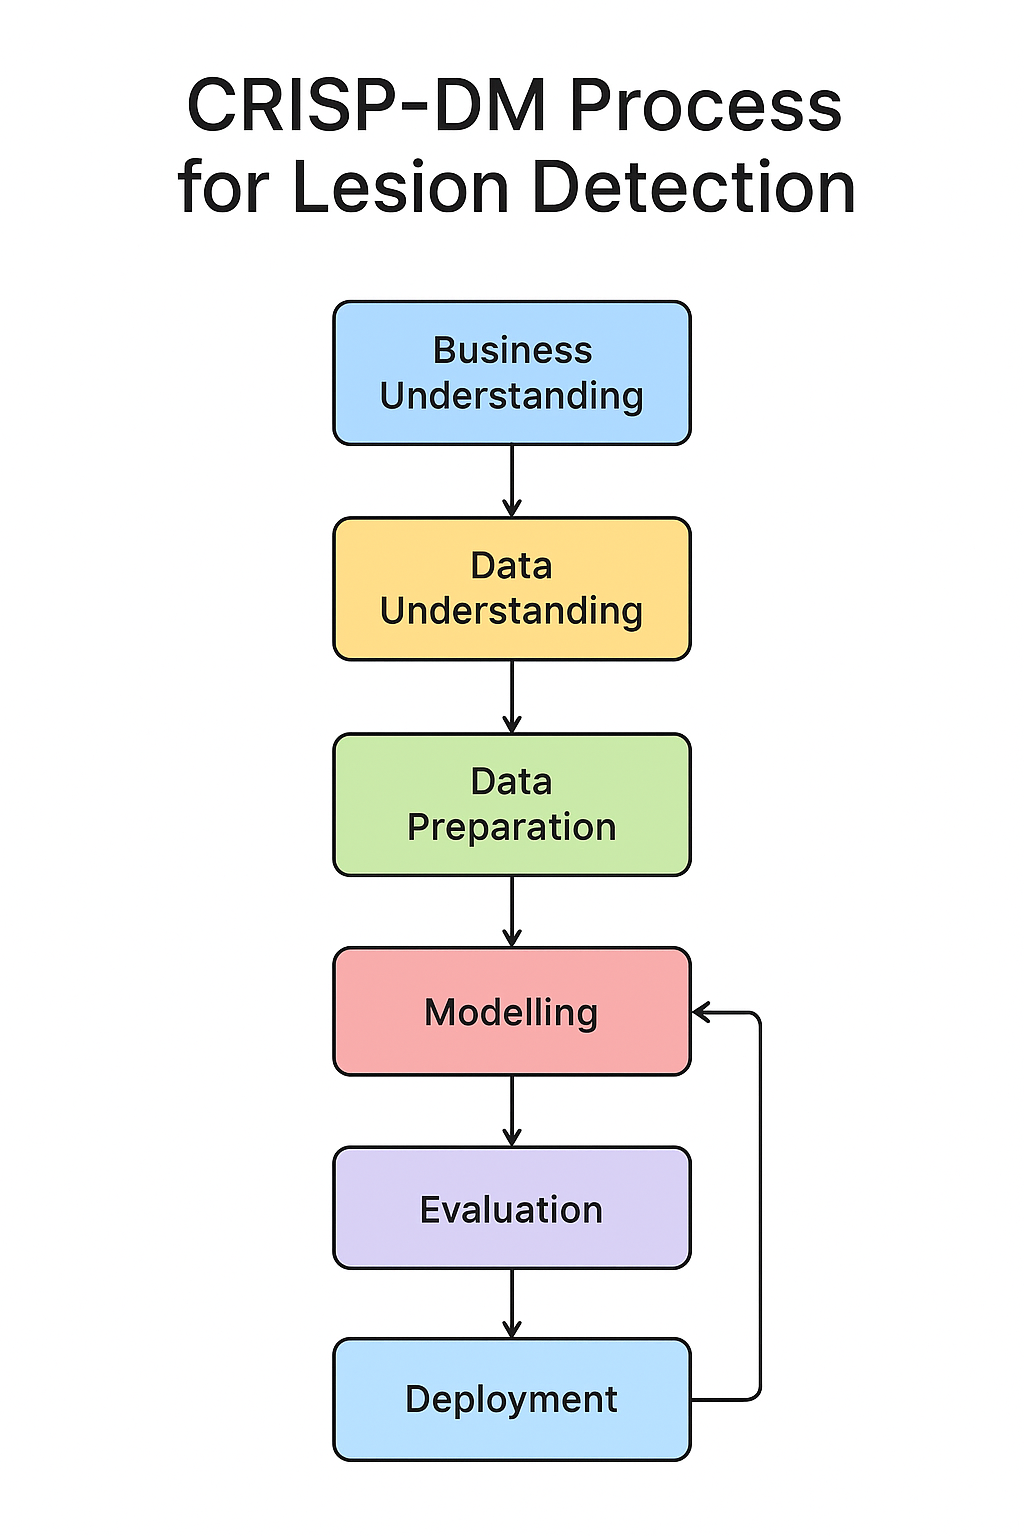
\includegraphics[keepaspectratio]{CRISP-DM-Diagram.png}}
\caption{CRISP-DM Process Diagram}
\end{figure}

\newpage

\subsection{Data and Requirements
Gathering}\label{data-and-requirements-gathering}

Requirements gathering is a critical stage in the development of any
complex system, particularly in healthcare-oriented artificial
intelligence (AI) applications. For a skin lesion detection and
classification system, eliciting accurate and comprehensive requirements
ensures that the technical design aligns with both medical best
practices and user expectations. This phase bridges the gap between the
theoretical capabilities of AI models and the practical needs of
end-users, which in this case include dermatologists, general
practitioners, researchers, and non-technical individuals seeking
self-assessment tools. As noted by Ruparelia
(\citeproc{ref-ruparelia2010software}{Ruparelia, 2010}), effective
requirements elicitation not only enhances system relevance but also
minimizes costly redesigns during later stages of development.

The approach adopted in this project combined multiple requirement
gathering methods, consistent with methodological recommendations in
software engineering and health informatics research
(\citeproc{ref-hay2006skin}{Hay et al., 2006};
\citeproc{ref-khan2021multi}{Khan et al., 2021}). Using a combination of
qualitative and quantitative strategies increased the robustness of our
findings by allowing cross-verification of insights (triangulation) and
by capturing both statistical trends and nuanced, context-specific
needs.

\subsubsection{Interviews}\label{interviews}

Semi-structured interviews were conducted with subject-matter experts,
particularly dermatologists, general practitioners, and AI researchers.
The purpose of these interviews was to explore diagnostic workflows,
common challenges in skin lesion assessment, and expectations for
integrating automated systems into clinical and teledermatology
practice. Interview questions were guided by literature on the adoption
of AI in dermatology (\citeproc{ref-esteva2017dermatologist}{Esteva et
al., 2017}; \citeproc{ref-zafar2023skin}{Zafar et al., 2023}) and
covered:

\begin{itemize}
\tightlist
\item
  The perceived accuracy and reliability thresholds acceptable for
  clinical decision support tools.
\item
  Preferred output formats (e.g., probability scores, lesion type
  classification, urgency recommendations).
\item
  Integration concerns with existing patient record systems and
  telemedicine platforms.
\item
  Ethical considerations, including patient consent and data privacy.
\end{itemize}

Interviews were audio-recorded, transcribed, and coded for thematic
analysis in later stages.

\subsubsection{Surveys and
Questionnaires}\label{surveys-and-questionnaires}

Two online survey instruments were designed, one targeting technical and
health professionals, and another aimed at non-technical individuals.
The former included domain-specific questions regarding AI model
transparency, explainability, and integration with clinical workflows,
while the latter focused on usability, trust, and perceived usefulness
of the proposed system.

The surveys comprised both closed-ended questions (for quantitative
analysis) and open-ended prompts (for qualitative insights).
Distribution was carried out via professional mailing lists, social
media groups, and university networks. In line with Hay et al.
(\citeproc{ref-hay2006skin}{Hay et al., 2006}), survey design
incorporated clear definitions of medical terms to ensure comprehension
among non-specialist respondents.

\subsubsection{Documentation Review}\label{documentation-review}

In addition to primary data collection, a review of relevant
documentation was undertaken. This included:

\begin{itemize}
\tightlist
\item
  Published clinical guidelines for skin cancer detection and
  management.
\item
  Existing research on automated lesion detection and classification
  (\citeproc{ref-kassem2021machine}{Kassem et al., 2021};
  \citeproc{ref-ogudo2023optimal}{Ogudo et al., 2023}).
\item
  Technical specifications of public skin lesion datasets such as
  HAM10000 (\citeproc{ref-tschandl2018ham10000}{Tschandl et al., 2018}).
\item
  Regulatory standards related to AI in healthcare, including data
  protection protocols.
\end{itemize}

The documentation review informed the selection of lesion categories,
the choice of evaluation metrics, and constraints for model deployment.

\subsubsection{Focus Groups}\label{focus-groups}

Focus groups were organized with a mixed composition of technical
experts, medical practitioners, and potential end-users. Unlike
individual interviews, focus groups facilitated dynamic discussions that
revealed collective priorities and concerns. For example, non-technical
users expressed apprehension about over-reliance on automated outputs
without human oversight, whereas clinicians emphasized the importance of
false negative minimization over overall accuracy.

\subsubsection{Synthesis of Findings}\label{synthesis-of-findings}

Findings from all methods were synthesized using a multi-step process:

\begin{enumerate}
\def\labelenumi{\arabic{enumi}.}
\tightlist
\item
  Extraction of key points from each method.
\item
  Cross-referencing to identify recurring requirements.
\item
  Prioritization using the MoSCoW method (Must have, Should have, Could
  have, Won't have) as recommended in agile software
  development(\citeproc{ref-srivastava2017scrum}{Srivastava et al.,
  2017}).
\end{enumerate}

This synthesis process ensured that the final requirements specification
incorporated both the functional and non-functional needs of diverse
stakeholders, and that the resulting system design balanced technical
feasibility with practical utility.

\subsection{Population and Sample}\label{population-and-sample}

\subsubsection{Target Population}\label{target-population}

The target population for this study consisted of individuals and groups
who would either directly use or influence the adoption of the proposed
skin lesion detection and classification system. This included:

\begin{itemize}
\tightlist
\item
  \textbf{Health Professionals}: Dermatologists, general practitioners,
  and other medical personnel involved in skin disease diagnosis and
  treatment. Their expertise was vital in validating clinical accuracy
  requirements, determining acceptable error thresholds, and ensuring
  the system aligned with established diagnostic workflows
  (\citeproc{ref-esteva2017dermatologist}{Esteva et al., 2017};
  \citeproc{ref-hay2006skin}{Hay et al., 2006}).\\
\item
  \textbf{Technical Experts}: Machine learning researchers, computer
  vision engineers, and software developers with experience in
  healthcare applications. Their input guided architectural design
  choices, algorithm selection, and system integration strategies
  (\citeproc{ref-khan2021multi}{Khan et al., 2021}).\\
\item
  \textbf{Non-Technical Individuals}: Members of the general public,
  particularly those with limited access to dermatological services.
  This group provided insight into usability, accessibility, and trust
  factors, especially in contexts where teledermatology may serve as a
  first point of consultation (\citeproc{ref-zafar2023skin}{Zafar et
  al., 2023}).
\end{itemize}

\subsubsection{Sampling Strategy}\label{sampling-strategy}

Given the diversity of the target population, a \textbf{stratified
sampling approach} was adopted, dividing respondents into two broad
strata:

\begin{enumerate}
\def\labelenumi{\arabic{enumi}.}
\tightlist
\item
  \textbf{Technical and Health Professionals} --- selected using
  \textbf{purposive sampling}, ensuring that only individuals with
  relevant domain knowledge and professional experience were included.
  Recruitment was facilitated through professional associations,
  academic networks, and LinkedIn outreach.\\
\item
  \textbf{Non-Technical Individuals} --- selected using
  \textbf{convenience sampling}, leveraging community networks, social
  media outreach, and university mailing lists. This method was chosen
  for its practicality and efficiency in reaching a large pool of
  respondents in a limited timeframe.
\end{enumerate}

This mixed approach ensured both the depth of expert feedback and the
breadth of general user perspectives.

\subsubsection{Sample Size}\label{sample-size}

A total of \textbf{25} responses were collected from technical and
health professionals, and \textbf{50} responses from non-technical
individuals. While the sample size for each group was constrained by
resource availability and the duration of the requirement gathering
phase, it was sufficient to capture recurring patterns and requirements
for system design.

\subsubsection{Justification of Sample
Size}\label{justification-of-sample-size}

In requirement elicitation for specialized healthcare AI systems, depth
of insight is often more critical than sheer volume of responses
(\citeproc{ref-ruparelia2010software}{Ruparelia, 2010}). For technical
and health professionals, a smaller but highly relevant participant pool
can yield actionable requirements without unnecessary redundancy. The
non-technical sample size, while larger, was chosen to ensure diversity
in age, education, and technology literacy, thereby reflecting the
heterogeneity of potential end-users.

\subsubsection{Limitations of Sampling
Approach}\label{limitations-of-sampling-approach}

Despite its effectiveness, the sampling approach had limitations:

\begin{itemize}
\tightlist
\item
  \textbf{Selection Bias}: Purposive sampling may have excluded certain
  professional subgroups, particularly in rural or resource-limited
  regions.
\item
  \textbf{Geographical Constraints}: The majority of respondents were
  located in urban centers, potentially under-representing rural
  healthcare contexts where teledermatology may have the highest impact.
\item
  \textbf{Response Bias}: Online surveys can disproportionately attract
  participants with higher digital literacy, possibly skewing usability
  feedback.
\end{itemize}

These limitations are acknowledged and considered when interpreting the
requirement gathering results and in the subsequent system design
stages.

\subsection{Quantitative Analysis}\label{quantitative-analysis}

\subsubsection{Data Analysis Techniques}\label{data-analysis-techniques}

Quantitative analysis was performed on the closed-ended questions from
the surveys, focusing on numerical and categorical variables. The
primary objective was to extract measurable trends regarding user
expectations, clinical requirements, and perceived usability of the
proposed skin lesion detection system.

Descriptive statistics, including \textbf{mean}, \textbf{median},
\textbf{mode}, and \textbf{standard deviation}, were calculated for
ordinal and interval-scale responses. For nominal data, frequency
distributions and percentages were computed. Cross-tabulation was
employed to explore potential relationships between demographic
variables (e.g., profession, years of experience, age group) and
perceptions of the system (\citeproc{ref-hay2006skin}{Hay et al., 2006};
\citeproc{ref-ruparelia2010software}{Ruparelia, 2010}).

To ensure robustness, data analysis adhered to established guidelines
for handling mixed healthcare and technology survey data
(\citeproc{ref-khan2021multi}{Khan et al., 2021}). Data cleaning
included the removal of incomplete responses and the normalization of
Likert-scale entries for comparability across questions.

\subsubsection{Data Visualization}\label{data-visualization}

Data visualization was used extensively to communicate quantitative
findings clearly. Bar charts, pie charts, and stacked column graphs were
employed to depict categorical distributions, while histograms
illustrated the spread of numerical responses. For relationship
analysis, clustered bar charts and side-by-side box plots were applied.

For example:

\begin{itemize}
\tightlist
\item
  Distribution of confidence levels in AI-assisted diagnosis among
  professionals versus non-technical users.
\item
  Comparative importance ratings of system features such as
  \textbf{diagnosis speed}, \textbf{accuracy}, and
  \textbf{explainability}.
\item
  Patterns in willingness to adopt the system across different age
  groups.
\end{itemize}

Visualizations were produced using spreadsheet software and statistical
tools, ensuring clarity for both technical and non-technical audiences.

\subsubsection{Interpretation and
Findings}\label{interpretation-and-findings}

Quantitative results revealed several key trends:

\begin{itemize}
\tightlist
\item
  \textbf{Accuracy Thresholds}: Health professionals consistently
  identified a minimum acceptable accuracy rate above 90\% for clinical
  decision support, while non-technical users were more tolerant of
  slightly lower accuracy levels if accompanied by clear explanations
  (\citeproc{ref-esteva2017dermatologist}{Esteva et al., 2017}).
\item
  \textbf{Feature Prioritization}: Across both groups, the most highly
  rated features were real-time analysis, mobile accessibility, and
  privacy safeguards.
\item
  \textbf{Adoption Willingness}: Willingness to adopt was highest among
  younger respondents and those with prior telemedicine experience,
  suggesting that digital familiarity positively influences acceptance.
\end{itemize}

These findings highlight the importance of tailoring the system's
feature set and communication style to different user categories.

\subsubsection{Conclusion}\label{conclusion}

The quantitative analysis provided objective, measurable insights into
user requirements and priorities. By quantifying trends and preferences,
the results served as a foundation for setting design specifications,
performance benchmarks, and usability targets. This ensured that
subsequent system development steps were guided by evidence-based
requirements rather than assumptions.

\subsection{Qualitative Analysis}\label{qualitative-analysis}

\subsubsection{Thematic Analysis
Approach}\label{thematic-analysis-approach}

Qualitative analysis was conducted on the open-ended survey responses,
interview transcripts, and focus group discussions. The primary
objective was to identify recurring themes, contextual nuances, and
stakeholder concerns that could not be captured through purely numerical
measures.

A \textbf{thematic analysis} approach was adopted, following the steps
outlined by Braun and Clarke (\citeproc{ref-braun2006using}{Braun \&
Clarke, 2006})*:

\begin{enumerate}
\def\labelenumi{\arabic{enumi}.}
\tightlist
\item
  \textbf{Familiarization}: Repeated reading of the raw text data to
  immerse in the content and context.
\item
  \textbf{Initial Coding}: Assigning descriptive labels to meaningful
  segments of text, capturing both explicit statements and implied
  sentiments.
\item
  \textbf{Theme Development}: Grouping related codes into broader
  thematic categories.
\item
  \textbf{Reviewing Themes}: Cross-checking against the dataset to
  ensure themes accurately represented the participants' views.
\item
  \textbf{Defining and Naming Themes}: Refining theme descriptions for
  clarity and relevance.
\item
  \textbf{Reporting}: Selecting illustrative quotes to convey the
  essence of each theme.
\end{enumerate}

\subsubsection{Coding and
Categorization}\label{coding-and-categorization}

Responses were coded manually using spreadsheet-based coding tables.
This process produced multiple overarching categories:

\begin{itemize}
\tightlist
\item
  \textbf{Accuracy and Trust}: Emphasis on clinical reliability and the
  need for human oversight in diagnosis
  (\citeproc{ref-esteva2017dermatologist}{Esteva et al., 2017};
  \citeproc{ref-zafar2023skin}{Zafar et al., 2023}).
\item
  \textbf{Usability and Accessibility}: Concerns over interface
  simplicity, language localization, and mobile optimization for
  low-bandwidth environments.
\item
  \textbf{Privacy and Ethics}: Demand for strict compliance with data
  protection regulations and transparent data usage policies
  (\citeproc{ref-khan2021multi}{Khan et al., 2021}).
\item
  \textbf{Educational Value}: Interest in integrating explanations and
  visual aids to help users understand lesion classifications and
  potential risks.
\end{itemize}

\subsubsection{Interpretation of Qualitative
Findings}\label{interpretation-of-qualitative-findings}

The qualitative data revealed several insights that influenced design
decisions:

\begin{itemize}
\tightlist
\item
  \textbf{Differing Risk Tolerance}: Medical professionals prioritized
  minimizing false negatives, even at the cost of slightly lower overall
  accuracy, whereas non-technical users valued a balance between speed
  and reliability.
\item
  \textbf{Need for Explainability}: Across all groups, participants
  favored outputs accompanied by visual indicators and textual
  explanations, supporting findings in explainable AI literature.
\item
  \textbf{Cultural and Language Considerations}: Participants from
  non-English-speaking backgrounds stressed the importance of
  multilingual support for both the interface and educational materials.
\end{itemize}

These findings underscored the necessity of designing a system that is
not only technically sound but also socially and ethically acceptable.

\subsubsection{Conclusion}\label{conclusion-1}

By capturing and analyzing the rich detail of participants'
perspectives, the qualitative analysis complemented the quantitative
results, providing a holistic understanding of user and stakeholder
needs. The combination of both methods ensured that the system's design
was informed by statistically significant trends as well as the subtler,
contextual factors that can impact adoption and trust.

\subsection{Dataset Description and
Preprocessing}\label{dataset-description-and-preprocessing}

The dataset used in this study was curated from multiple open-source
dermatological image repositories and validated clinical sources. It
comprises high-quality images covering \textbf{33 unique skin condition
categories}, spanning viral, bacterial, fungal, parasitic, autoimmune,
inflammatory, and neoplastic conditions. Unlike conventional
dermatological datasets such as \textbf{HAM10000}, which focus
predominantly on melanocytic lesions (\citeproc{ref-khan2021multi}{Khan
et al., 2021}; \citeproc{ref-tschandl2018ham10000}{Tschandl et al.,
2018}), this dataset extends coverage to a broader spectrum of
dermatological manifestations, enabling a more versatile diagnostic
tool.

\subsubsection{Dataset Composition}\label{dataset-composition}

The dataset categories are as follows:

\begin{itemize}
\tightlist
\item
  \textbf{Viral Infections:} Chickenpox, Monkeypox, Measles, Shingles,
  Herpes, Cowpox.
\item
  \textbf{Bacterial Infections:} Impetigo, Leprosy, Whitlow.
\item
  \textbf{Fungal Infections:} Athlete's Foot, Ringworm, Nail Fungus.
\item
  \textbf{Parasitic Infestations:} Scabies, Tungiasis, Larva Migrans.
\item
  \textbf{Inflammatory and Autoimmune Conditions:} Eczema, Psoriasis,
  Autoimmune Disease, Rash Dermatitis, Vitiligo.
\item
  \textbf{Benign and Malignant Tumors:} Basal Cell Carcinoma (BCC),
  Squamous Cell Carcinoma (SCC), Actinic Keratosis, Melanoma, Nevus,
  Seborrheic Keratosis, Benign Tumor, Moles.
\item
  \textbf{Other Dermatological Conditions:} Acne, Neurofibromatosis,
  Vascular Lesion, Healthy skin.
\end{itemize}

This broad coverage is particularly valuable for \textbf{primary care
and teledermatology}, where non-specialist practitioners encounter
diverse skin pathologies (\citeproc{ref-adegun2020fcn}{Adegun \& Viriri,
2020}; \citeproc{ref-zafar2023skin}{Zafar et al., 2023}).

\subsubsection{Data Sources}\label{data-sources}

The dataset was compiled from:

\begin{itemize}
\tightlist
\item
  \textbf{Public dermatology datasets} --- e.g., HAM10000, ISIC Archive
  (for melanoma, nevus, keratosis, and carcinoma images).
\item
  \textbf{Open-access image repositories} --- curated collections for
  conditions such as chickenpox, monkeypox, and scabies.
\item
  \textbf{Institutional contributions} --- small-scale, ethically
  approved clinical image sets for rare conditions such as tungiasis and
  larva migrans.
\end{itemize}

All images were reviewed to ensure:

\begin{itemize}
\tightlist
\item
  Minimum resolution of 224×224 pixels before resizing.
\item
  Clear lesion visibility with minimal occlusions.
\item
  Correct disease labeling by source datasets.
\end{itemize}

\subsubsection{Dataset Distribution and Class
Imbalance}\label{dataset-distribution-and-class-imbalance}

The dataset is \textbf{imbalanced}:\\
Classes like \emph{Acne} and \emph{Eczema} have large sample counts,
while rare conditions such as \emph{Tungiasis} or \emph{Larva Migrans}
have far fewer. Such imbalance can bias models toward majority classes,
leading to reduced recall for rare categories
(\citeproc{ref-buda2018systematic}{Buda et al., 2018};
\citeproc{ref-kassem2021machine}{Kassem et al., 2021}).

Mitigation strategies applied:

\begin{itemize}
\tightlist
\item
  \textbf{Class weighting} --- Computed via
  \texttt{sklearn.utils.class\_weight} and incorporated into the
  cross-entropy loss.
\item
  \textbf{Data augmentation} --- Uniformly applied at runtime, with
  possible further targeted augmentation for minority classes in future
  iterations.
\end{itemize}

\begin{figure}

{\centering 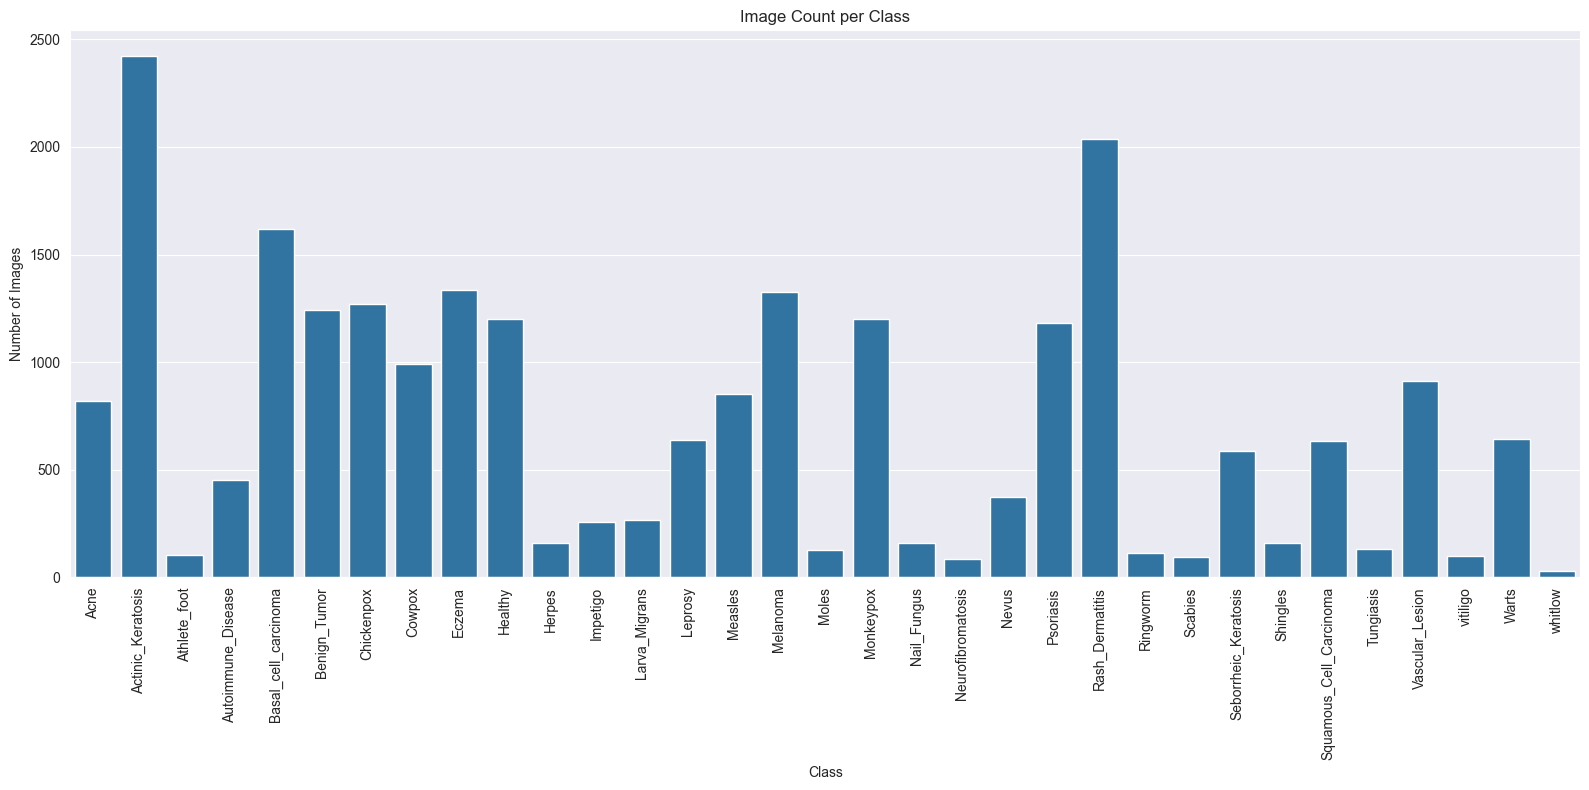
\includegraphics[width=1\linewidth]{images_per_class} 

}

\caption{Number of images per class}\label{fig:unnamed-chunk-1}
\end{figure}

\begin{figure}

{\centering 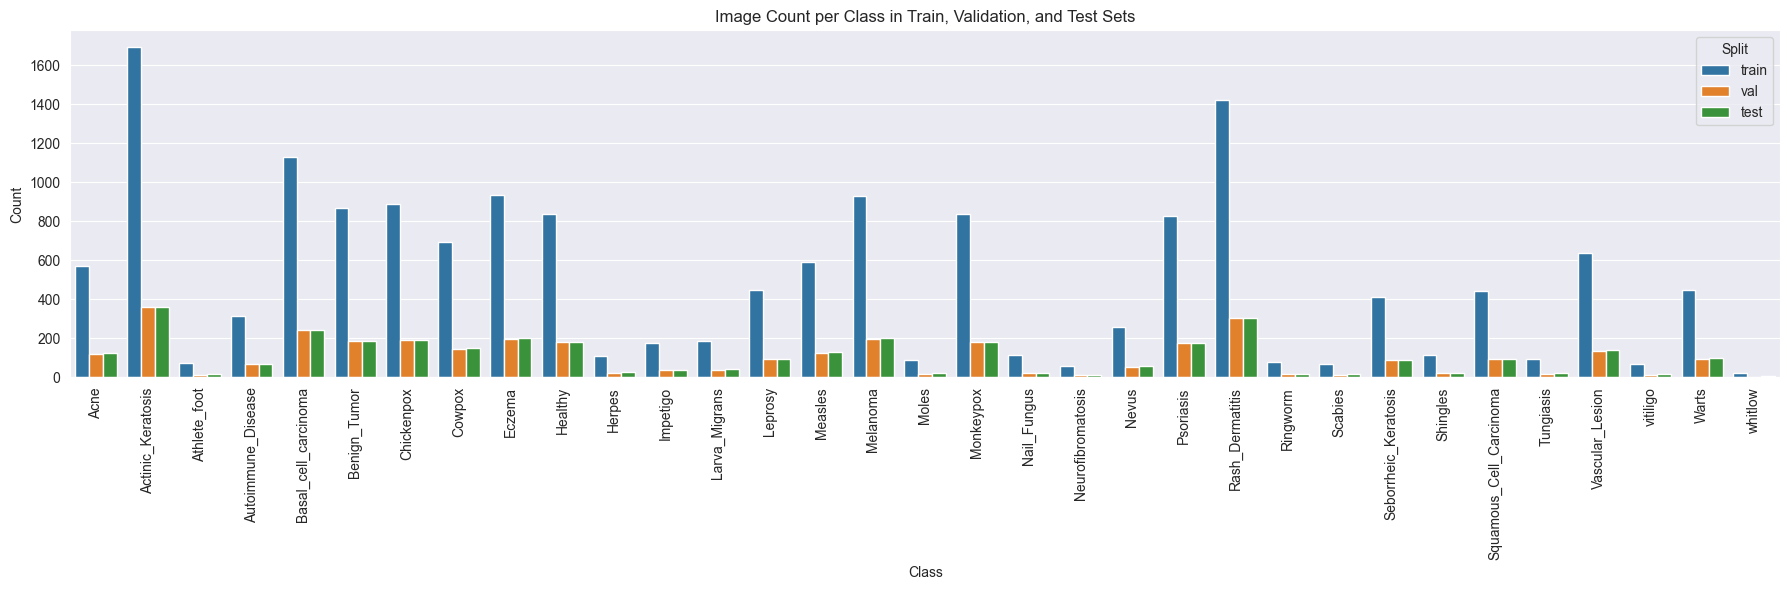
\includegraphics[width=1\linewidth]{class_distribution} 

}

\caption{Class distribution plot across splits}\label{fig:unnamed-chunk-2}
\end{figure}

\subsubsection{Data Partitioning}\label{data-partitioning}

Images were split into:

\begin{itemize}
\tightlist
\item
  \textbf{Training set:} 70\%
\item
  \textbf{Validation set:} 15\%
\item
  \textbf{Test set:} 15\%
\end{itemize}

Splitting was \textbf{stratified per class} to preserve class
proportions across sets, ensuring fair evaluation.

\subsubsection{Exploratory Data Analysis
(EDA)}\label{exploratory-data-analysis-eda}

Before training, \textbf{EDA} was conducted on the processed dataset to
assess its suitability:

\begin{enumerate}
\def\labelenumi{\arabic{enumi}.}
\tightlist
\item
  \textbf{Class distribution analysis} --- Generated bar plots to
  visualize image counts per class for each dataset split, confirming
  imbalance patterns.
\item
  \textbf{Sample inspection} --- Random samples per class were displayed
  to verify label correctness and assess intra-class variability.
\item
  \textbf{Image dimension profiling} --- Recorded resolutions and aspect
  ratios from random subsets to guide resizing and padding strategies.
\end{enumerate}

\begin{figure}

{\centering 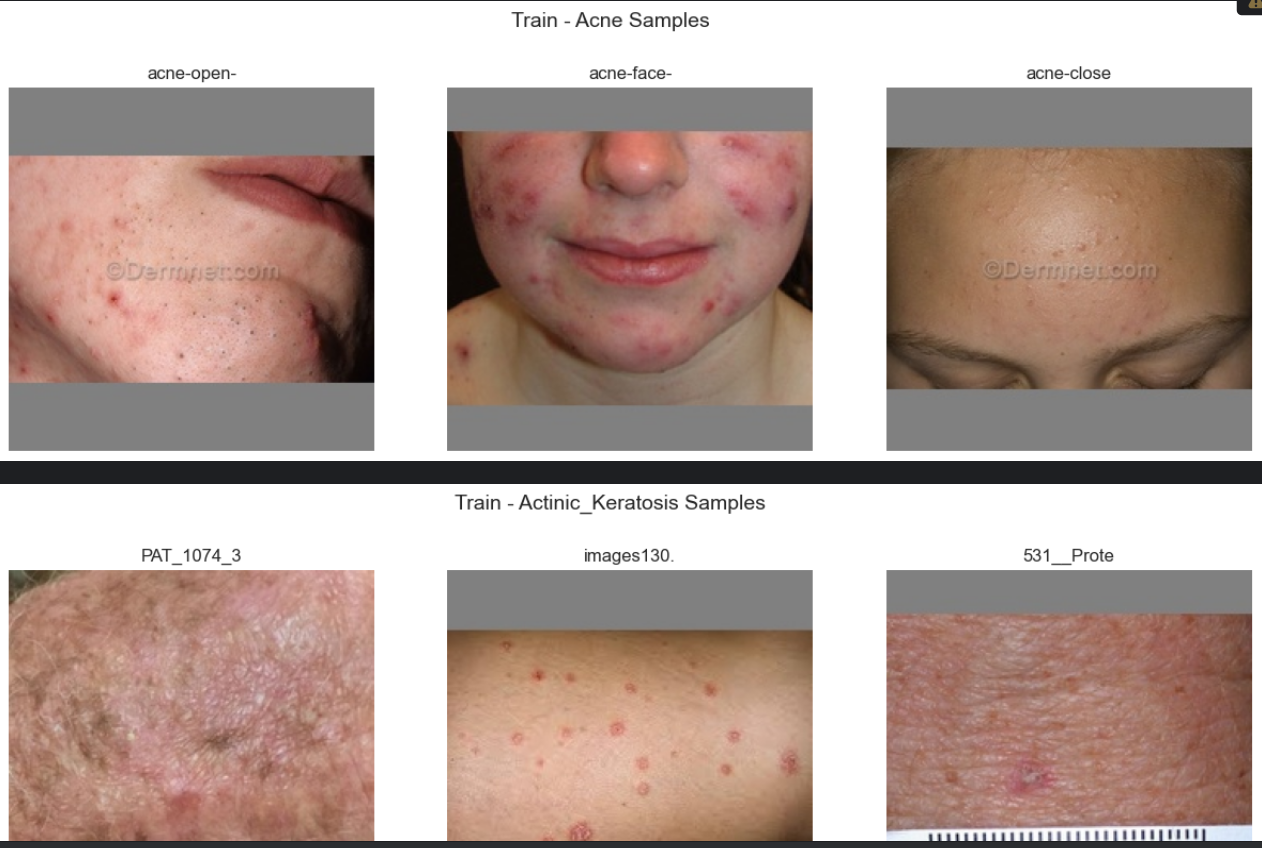
\includegraphics[width=1\linewidth]{class_sample_images} 

}

\caption{Example sample images per class}\label{fig:unnamed-chunk-3}
\end{figure}

\subsubsection{Preprocessing Pipeline}\label{preprocessing-pipeline}

A reproducible preprocessing pipeline was implemented in Python,
combining \textbf{offline standardization} and \textbf{online
augmentation}:

\paragraph{Offline Processing}\label{offline-processing}

\begin{itemize}
\tightlist
\item
  \textbf{Image Conversion} --- Ensured all images were in RGB mode to
  match the pretrained ResNet input format.
\item
  \textbf{Resizing with Padding} --- Used \textbf{Lanczos resampling} to
  resize while preserving aspect ratio, padding with a neutral grey
  background (128, 128, 128) to reach 224×224 pixels.
\item
  \textbf{Format Standardization} --- Saved all outputs as high-quality
  JPEG files for consistency.
\item
  \textbf{Directory Structuring} --- Images organized into
  \texttt{train}, \texttt{val}, and \texttt{test} directories by class.
\end{itemize}

\paragraph{Online Augmentation (During
Training)}\label{online-augmentation-during-training}

\begin{longtable}[]{@{}
  >{\raggedright\arraybackslash}p{(\linewidth - 4\tabcolsep) * \real{0.1905}}
  >{\raggedright\arraybackslash}p{(\linewidth - 4\tabcolsep) * \real{0.4048}}
  >{\raggedright\arraybackslash}p{(\linewidth - 4\tabcolsep) * \real{0.4048}}@{}}
\toprule\noalign{}
\begin{minipage}[b]{\linewidth}\raggedright
Transformation
\end{minipage} & \begin{minipage}[b]{\linewidth}\raggedright
Purpose
\end{minipage} & \begin{minipage}[b]{\linewidth}\raggedright
Parameters
\end{minipage} \\
\midrule\noalign{}
\endhead
\bottomrule\noalign{}
\endlastfoot
Random Horizontal Flip & Simulate left/right lesion orientation & p =
0.5 \\
Random Rotation & Account for patient positioning differences & ±10° \\
Color Jitter & Simulate lighting variations & brightness=0.2,
contrast=0.2, saturation=0.2 \\
Normalization & Match ImageNet statistics & mean={[}0.485, 0.456,
0.406{]}, std={[}0.229, 0.224, 0.225{]} \\
\end{longtable}

These augmentations improve generalization and reduce overfitting
(\citeproc{ref-lecun2015deep}{LeCun et al., 2015};
\citeproc{ref-mahbod2019skin}{Mahbod et al., 2019}).

\subsubsection{Impact of Preprocessing and
Augmentation}\label{impact-of-preprocessing-and-augmentation}

The chosen preprocessing and augmentation steps:

\begin{itemize}
\tightlist
\item
  Improved robustness to variations in lighting, camera quality, and
  orientation.
\item
  Reduced the risk of overfitting by diversifying the training data.
\item
  Preserved lesion geometry, which is essential for dermatology-specific
  feature learning.
\end{itemize}

\subsection{Model Architecture}\label{model-architecture}

The classification model is based on a \textbf{fine-tuned ResNet-18}
(\citeproc{ref-he2016deep}{He et al., 2016}), selected for its favorable
trade-off between accuracy and computational cost. This architecture is
well-suited for mobile and edge deployment due to its small parameter
count and competitive accuracy in medical image tasks
(\citeproc{ref-esteva2017dermatologist}{Esteva et al., 2017}).

\subsubsection{Baseline Architecture}\label{baseline-architecture}

ResNet-18 comprises:

\begin{itemize}
\tightlist
\item
  An initial convolutional layer (7×7 kernel, stride 2) followed by
  batch normalization and ReLU activation.
\item
  Four sequential residual blocks (layers 1--4) with skip connections to
  facilitate gradient flow.
\item
  Global average pooling, followed by a fully connected (fc) layer for
  classification.
\end{itemize}

\subsubsection{Transfer Learning
Adaptations}\label{transfer-learning-adaptations}

To adapt ResNet-18 for multi-class lesion classification:

\begin{itemize}
\tightlist
\item
  \textbf{Weights} initialized from ImageNet-pretrained ResNet-18
  (\texttt{ResNet18\_Weights.DEFAULT}).
\item
  \textbf{Frozen layers:} Layers 1--3 kept frozen to retain generic
  visual features.
\item
  \textbf{Unfrozen layers:} Layer 4 and the fc layer trained for
  dermatology-specific adaptation.
\item
  \textbf{Modified final layer:} Replaced \texttt{fc} with
  \texttt{nn.Linear(512,\ 33)} for 33-class output.
\end{itemize}

This selective fine-tuning strategy combines pretrained low- and
mid-level feature extraction with high-level feature specialization
(\citeproc{ref-yosinski2014transfer}{Yosinski et al., 2014}).

\subsubsection{Loss Function and Class
Balancing}\label{loss-function-and-class-balancing}

A \textbf{weighted cross-entropy loss} was employed, where each class
weight was inversely proportional to its frequency in the training set.
This approach ensured that minority classes contributed more to gradient
updates, improving detection rates for rare conditions.

\subsubsection{Optimization and
Regularization}\label{optimization-and-regularization}

Training configuration:

\begin{itemize}
\tightlist
\item
  \textbf{Optimizer:} Adam (\texttt{lr=0.001},
  \texttt{weight\_decay=1e-4}).
\item
  \textbf{Scheduler:} ReduceLROnPlateau (factor=0.5, patience=2).
\item
  \textbf{Early Stopping:} Stop if validation loss fails to improve for
  5 epochs.
\item
  \textbf{Batch Size:} 32.
\end{itemize}

Regularization via L2 weight decay and early stopping reduced
overfitting, while dynamic learning rate adjustment improved convergence
stability.

\subsubsection{Rationale for ResNet-18
Selection}\label{rationale-for-resnet-18-selection}

ResNet-18 was chosen because:

\begin{enumerate}
\def\labelenumi{\arabic{enumi}.}
\tightlist
\item
  It delivers high accuracy with relatively low inference time.
\item
  Prior studies confirm ResNet's effectiveness for skin lesion
  classification (\citeproc{ref-albahar2019skin}{Albahar, 2019};
  \citeproc{ref-harangi2018skin}{Harangi, 2018}).
\item
  Its moderate depth supports deployment on resource-constrained devices
  without heavy hardware requirements.
\end{enumerate}

\begin{figure}

{\centering 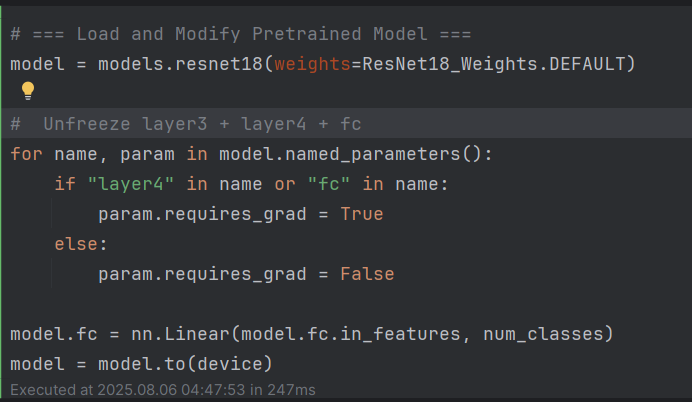
\includegraphics[width=1\linewidth]{unfrozen_layers} 

}

\caption{Modified ResNet-18 highlighting unfrozen layers}\label{fig:unnamed-chunk-4}
\end{figure}

\subsection{Training Strategy}\label{training-strategy}

The training phase was carefully designed to achieve a balance between
\textbf{computational efficiency}, \textbf{classification accuracy}, and
\textbf{generalization capability} to unseen images. This section
describes the training configuration, rationale for hyperparameter
selection, and mechanisms adopted to handle the inherent challenges of
medical image classification.

\subsubsection{Hardware and Frameworks}\label{hardware-and-frameworks}

All model training was conducted on a GPU-enabled workstation equipped
with CUDA support. This significantly reduced training time compared to
CPU-based execution, enabling faster experimentation and hyperparameter
tuning. The model was implemented in \textbf{PyTorch}, chosen for its
flexibility and strong community support in research-oriented deep
learning tasks. Supporting libraries included:

\begin{itemize}
\tightlist
\item
  \textbf{torchvision} for pretrained model loading and image
  transformation pipelines.
\item
  \textbf{scikit-learn} for computing class weights and auxiliary
  evaluation metrics.
\item
  \textbf{tqdm} for real-time progress tracking.
\item
  \textbf{TensorBoard} for monitoring loss, accuracy, and learning rate
  trends over epochs.
\end{itemize}

\subsubsection{Data Loading and
Batching}\label{data-loading-and-batching}

The processed dataset (Section 3.3) was loaded via PyTorch's
\texttt{DataLoader} class with the following configurations:

\begin{itemize}
\tightlist
\item
  \textbf{Batch Size:} 32 images per iteration --- a compromise between
  computational efficiency and GPU memory constraints.
\item
  \textbf{Shuffling:} Enabled for the training set to ensure diverse
  sample exposure per batch, breaking any inherent ordering in the data.
\item
  \textbf{Parallelism:} Four worker threads (\texttt{num\_workers=4})
  with a prefetch factor of four, minimizing idle GPU time due to data
  loading delays.
\end{itemize}

This setup ensured that each training iteration received a randomized,
memory-optimized batch, which has been shown to improve convergence
rates (\citeproc{ref-goodfellow2016deep}{Goodfellow et al., 2016}).

\subsubsection{Transfer Learning and Layer
Freezing}\label{transfer-learning-and-layer-freezing}

Given the limited availability of dermatological images for certain rare
conditions, training a deep convolutional neural network from scratch
was deemed impractical. Instead, \textbf{transfer learning} was employed
using a ResNet-18 architecture pretrained on the ImageNet dataset. The
transfer learning strategy included:

\begin{itemize}
\tightlist
\item
  \textbf{Freezing layers 1--3:} Preserving generic feature extractors
  (edges, textures, shapes) learned from the large-scale ImageNet
  dataset.
\item
  \textbf{Unfreezing layer 4 and the fully connected layer:} Allowing
  adaptation of higher-level feature representations to the unique
  textures and lesion patterns in dermatological images.
\item
  \textbf{Classifier replacement:} Modifying the final fully connected
  layer to output 33 logits corresponding to the target disease
  categories.
\end{itemize}

Selective unfreezing reduced the risk of overfitting while allowing
enough flexibility for domain adaptation
(\citeproc{ref-yap2018multimodal}{Yap et al., 2018}).

\subsubsection{Loss Function and Class
Balancing}\label{loss-function-and-class-balancing-1}

A major challenge identified during exploratory data analysis (EDA) was
\textbf{class imbalance}, with conditions like \emph{Eczema} and
\emph{Acne} having significantly more samples than rare diseases such as
\emph{Tungiasis} or \emph{Cowpox}. Without correction, the model would
bias predictions toward majority classes. To address this:

\begin{itemize}
\tightlist
\item
  \textbf{Weighted Cross-Entropy Loss} was used, with per-class weights
  computed using:
\end{itemize}

\[
w_c = \frac{N}{n_c \cdot K}
\]

where:

\begin{itemize}
\tightlist
\item
  \(N\) is the total number of training samples,
\item
  \(n_c\) is the sample count for class \(c\),
\item
  \(K\) is the number of classes.
\end{itemize}

These weights were passed directly to PyTorch's
\texttt{nn.CrossEntropyLoss}, ensuring that errors on minority classes
contributed proportionally more to gradient updates. This method is
well-supported in medical imaging literature for combating imbalance
(\citeproc{ref-krawczyk2016learning}{Krawczyk, 2016}).

\subsubsection{Optimization and Learning Rate
Scheduling}\label{optimization-and-learning-rate-scheduling}

Optimization was handled by the \textbf{Adam} optimizer with:

\begin{itemize}
\tightlist
\item
  Learning rate \(\alpha = 0.001\),
\item
  Weight decay \(= 1\times 10^{-4}\) for L2 regularization.
\end{itemize}

Adam was chosen for its adaptive learning rates and robustness to sparse
gradients (\citeproc{ref-adam2014method}{Adam et al., 2014}). To avoid
stagnation, the \texttt{ReduceLROnPlateau} scheduler was employed,
reducing the learning rate by a factor of 0.5 if validation loss failed
to improve for two consecutive epochs.

\subsubsection{Early Stopping}\label{early-stopping}

To prevent overfitting and unnecessary computation, \textbf{early
stopping} was implemented with a patience of 5 epochs, if no improvement
in validation loss was observed during this period, training terminated.
This approach aligns with best practices in deep learning model
regularization (\citeproc{ref-prechelt1998early}{Prechelt, 1998}).

\subsubsection{Epochs, Monitoring, and
Logging}\label{epochs-monitoring-and-logging}

The model was trained for a maximum of \textbf{20 epochs}. Real-time
metrics were logged to TensorBoard, capturing:

\begin{itemize}
\tightlist
\item
  Training and validation loss curves,
\item
  Training and validation accuracy curves,
\item
  Learning rate schedules.
\end{itemize}

\begin{figure}

{\centering 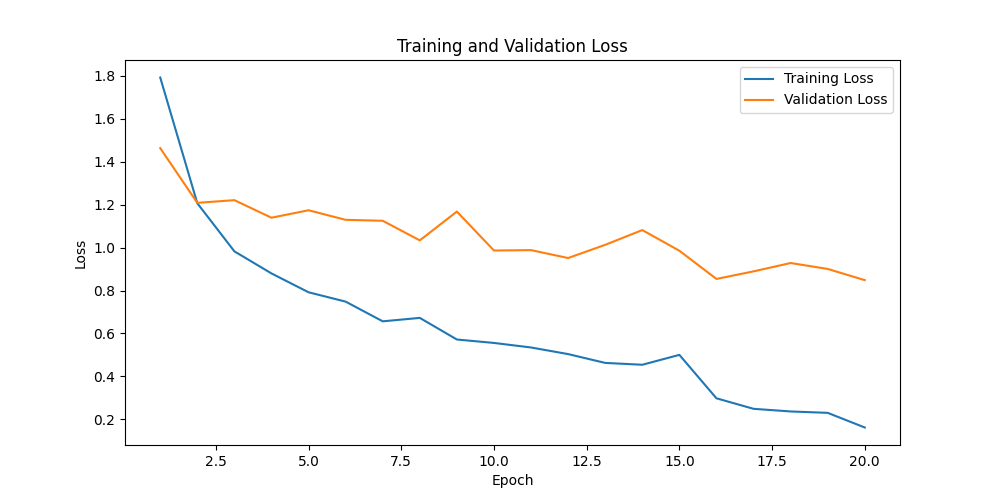
\includegraphics[width=1\linewidth]{loss_curve_v3} 

}

\caption{Training and validation loss curves}\label{fig:unnamed-chunk-5}
\end{figure}

\begin{figure}

{\centering 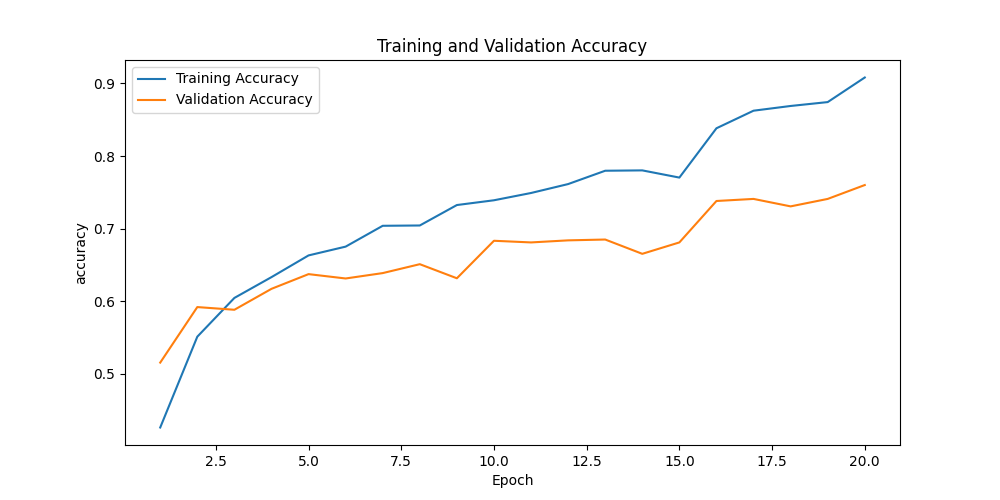
\includegraphics[width=1\linewidth]{accuracy_curve_v3} 

}

\caption{Training and validation accuracy curves}\label{fig:unnamed-chunk-6}
\end{figure}

\subsection{Evaluation Strategy}\label{evaluation-strategy}

The evaluation methodology was designed to quantify not only the
\textbf{overall classification performance} but also the
\textbf{per-class diagnostic reliability}, given the medical context of
the task.

\subsubsection{Test Set Protocol}\label{test-set-protocol}

All reported results are based on the \textbf{test set}, which was
strictly isolated from training and validation data to ensure unbiased
performance estimates. This set simulates real-world deployment
conditions by containing images unseen by the model at any training
stage.

\subsubsection{Evaluation Metrics}\label{evaluation-metrics}

Given the dataset imbalance and the multi-class nature of the problem,
we employed the following metrics:

\begin{itemize}
\tightlist
\item
  \textbf{Accuracy:} \[
  \text{Accuracy} = \frac{\text{Number of correct predictions}}{\text{Total number of predictions}}
  \]
\end{itemize}

While intuitive, accuracy alone may mask poor minority-class performance
in imbalanced datasets.

\begin{itemize}
\tightlist
\item
  \textbf{Precision (per class and macro-averaged):} \[
  \text{Precision} = \frac{\text{True Positives}}{\text{True Positives} + \text{False Positives}}
  \]
\end{itemize}

Precision is critical in medical applications where false positives can
lead to unnecessary anxiety or treatment.

\begin{itemize}
\tightlist
\item
  \textbf{Recall / Sensitivity:} \[
  \text{Recall} = \frac{\text{True Positives}}{\text{True Positives} + \text{False Negatives}}
  \]
\end{itemize}

High recall ensures that most true cases are detected, reducing missed
diagnoses.

\begin{itemize}
\tightlist
\item
  \textbf{F1-Score:} \[
  \text{F1} = 2 \times \frac{\text{Precision} \times \text{Recall}}{\text{Precision} + \text{Recall}}
  \]
\end{itemize}

Balances the trade-off between precision and recall.

\begin{itemize}
\tightlist
\item
  \textbf{Confusion Matrix:}
\end{itemize}

Visualizes per-class prediction performance and highlights common
misclassifications (e.g., \emph{Seborrheic Keratosis} misclassified as
\emph{Actinic Keratosis}).

\begin{itemize}
\tightlist
\item
  \textbf{ROC AUC (One-vs-Rest):} Measures separability between each
  class and all others, providing insight into decision threshold
  robustness.
\end{itemize}

\subsubsection{Rationale for Metric
Selection}\label{rationale-for-metric-selection}

These metrics were selected based on clinical relevance. In dermatology
AI, high recall is often prioritized to minimize missed malignant cases,
while high precision reduces unnecessary biopsies or referrals.
Macro-averaging ensures all classes contribute equally to the overall
performance measure, regardless of prevalence.

\subsubsection{Additional Performance
Considerations}\label{additional-performance-considerations}

Given the intended integration into a \textbf{CLI} for research and a
\textbf{React Native} mobile application, additional evaluations were
made on:

\begin{itemize}
\tightlist
\item
  \textbf{Inference latency} --- to ensure acceptable response times on
  standard mobile hardware.
\item
  \textbf{Model size and memory footprint} --- to confirm feasibility
  for mobile and edge deployment.
\end{itemize}

\subsubsection{Visualizations}\label{visualizations}

Performance visualizations will be added to the final report:

\begin{itemize}
\tightlist
\item
  Loss and accuracy curves across epochs,
\item
  Confusion matrix heatmap for error analysis,
\item
  ROC curves for multi-class separability assessment.
\end{itemize}

These plots aid in communicating results to both technical and clinical
audiences.

\subsection{System Deployment}\label{system-deployment}

The deployment phase transforms the trained skin lesion classification
model into a functional application ecosystem that is accessible to both
researchers and end-users. This involves integrating the AI model into
multiple delivery channels, a \textbf{command-line interface (CLI)} for
advanced research workflows, and a \textbf{React Native mobile
application} for primary care and public health use. Deployment
considerations also include hosting infrastructure, scalability, data
privacy, and regulatory compliance.

\subsubsection{Deployment Objectives}\label{deployment-objectives}

The system deployment aims to:

\begin{enumerate}
\def\labelenumi{\arabic{enumi}.}
\tightlist
\item
  \textbf{Ensure accessibility} --- enable both technical and
  non-technical users to interact with the model.
\item
  \textbf{Maintain efficiency} --- achieve low-latency inference, even
  on resource-constrained devices.
\item
  \textbf{Support scalability} --- allow expansion to larger datasets,
  additional disease classes, and multi-language support.
\item
  \textbf{Facilitate integration} --- ensure the model can be embedded
  into broader healthcare systems or telemedicine platforms.
\end{enumerate}

\subsubsection{Command-Line Interface (CLI) for
Researchers}\label{command-line-interface-cli-for-researchers}

The CLI is designed to serve dermatology researchers and data scientists
who require batch processing, model experimentation, and in-depth
performance analytics.

\paragraph{Key Features:}\label{key-features}

\begin{itemize}
\tightlist
\item
  \textbf{Single-image and batch prediction modes}\\
  Researchers can run predictions on individual lesion images or entire
  folders.
\item
  \textbf{Output formats}\\
  Predictions can be saved in CSV/JSON format, containing the predicted
  class, confidence scores, and timestamp.
\item
  \textbf{Model evaluation tools}\\
  Researchers can compute metrics such as accuracy, precision, recall,
  F1-score, and generate confusion matrices on new datasets.
\item
  \textbf{Custom model loading}\\
  Allows researchers to test alternative trained models by specifying
  the path via a command-line argument.
\end{itemize}

\subsubsection{Mobile Application for
End-Users}\label{mobile-application-for-end-users}

The React Native mobile application is intended for healthcare
practitioners, field workers, and potentially patients for preliminary
lesion screening.\\
The app will integrate the trained ResNet-18 model either
\textbf{on-device} (for offline capability) or via \textbf{cloud-hosted
inference APIs} (for lighter device workloads).

\paragraph{Core Features:}\label{core-features}

\begin{itemize}
\tightlist
\item
  \textbf{Image Capture \& Upload}\\
  Users can capture lesion images directly via the phone's camera or
  upload from the gallery.
\item
  \textbf{Instant Classification}\\
  The app provides top predictions with confidence scores.
\item
  \textbf{Educational Content}\\
  Displays information about predicted conditions, including symptoms
  and recommended next steps.
\item
  \textbf{Offline Mode (Planned)}\\
  A lightweight, quantized version of the model can be embedded for use
  in low-connectivity regions.
\end{itemize}

\subsubsection{Hosting and API
Infrastructure}\label{hosting-and-api-infrastructure}

The system will be deployed using a \textbf{serverless cloud
architecture} on Amazon Web Services (AWS). This approach was selected
to ensure scalability, cost efficiency, and simplified maintenance. Key
components include:

\begin{itemize}
\tightlist
\item
  \textbf{Amazon API Gateway} -- Handles user requests and routes them
  securely to backend services.\\
\item
  \textbf{AWS Lambda} -- Executes serverless functions for
  classification inference, enrichment processing, and result handling,
  with automatic scaling based on demand.\\
\item
  \textbf{Amazon S3 (on Outposts)} -- Provides secure and reliable
  storage for the trained model and related assets.\\
\item
  \textbf{Amazon SQS} -- Manages asynchronous request queues to decouple
  processes and enhance reliability.\\
\item
  \textbf{Amazon DynamoDB} -- Serves as the primary database for storing
  predictions, enriched descriptions, and user-related data.\\
\item
  \textbf{OpenAI LLM Integration} -- Provides automated text enrichment
  for clinical explanations and user-friendly feedback.
\end{itemize}

This configuration eliminates the need for dedicated server management,
reduces operational overhead, and ensures the system can seamlessly
scale to accommodate varying user loads. Furthermore, the
\textbf{pay-per-use billing model} minimizes costs during periods of low
activity, making the solution sustainable in both testing and production
environments.

\subsubsection{Deployment Workflow}\label{deployment-workflow}

The deployment workflow includes:

\begin{enumerate}
\def\labelenumi{\arabic{enumi}.}
\item
  \textbf{Model Export} --- trained model saved in \texttt{.pth} and
  \texttt{.pt} formats for compatibility with both PyTorch and
  TorchScript (mobile deployment).
\item
  \textbf{API Development} --- RESTful API endpoints for:

  \begin{itemize}
  \tightlist
  \item
    \texttt{/predict} --- accept image input, return classification
    results.
  \item
    \texttt{/health} --- server health check.
  \item
    \texttt{/version} --- current model version.
  \end{itemize}
\item
  \textbf{Integration Testing} --- ensuring consistent predictions
  across CLI, mobile, and API-based requests.
\item
  \textbf{Security and Privacy} --- enforce HTTPS for data transfer,
  anonymize image metadata, and comply with GDPR/HIPAA standards where
  applicable.
\end{enumerate}

\subsubsection{Monitoring and
Maintenance}\label{monitoring-and-maintenance}

Post-deployment, the system will include:

\begin{itemize}
\tightlist
\item
  \textbf{Usage analytics} --- monitor API requests, app downloads, and
  prediction frequency.
\item
  \textbf{Model performance tracking} --- periodic testing with new data
  to detect performance drift.
\item
  \textbf{Continuous improvement cycle} --- retraining with new cases,
  including rare or misclassified conditions.
\end{itemize}

\subsection{Summary of Methodology}\label{summary-of-methodology}

This chapter presented the complete methodology adopted for the design,
development, training, and deployment of the proposed \textbf{skin
lesion detection and classification system}. The approach was guided by
the \textbf{CRISP-DM} framework, ensuring that every stage, from problem
definition to system deployment, followed a structured, iterative, and
evidence-driven process.

The \textbf{business understanding phase} established the project's core
objective: to develop a multi-condition dermatological diagnostic aid
that can assist healthcare practitioners and researchers by classifying
a wide range of skin lesions. Unlike many prior works such as those
based on the HAM10000 dataset, which focus primarily on melanoma and a
few related conditions, our system targets \textbf{33 unique
dermatological conditions} spanning viral, bacterial, fungal, parasitic,
autoimmune, inflammatory, and neoplastic categories. This broad coverage
is intended to make the system more relevant in \textbf{primary care,
rural healthcare, and teledermatology contexts}, where clinicians may
encounter a diverse set of skin disorders.

The \textbf{data understanding phase} involved collecting images from
multiple open-source dermatology datasets, open-access medical
repositories, and selected institutional sources. Exploratory Data
Analysis (EDA) was conducted to assess the dataset's structure, identify
imbalances, and verify image quality. The EDA included:

\begin{itemize}
\tightlist
\item
  \textbf{Class distribution analysis}, revealing significant imbalances
  (e.g., Acne and Eczema having hundreds of samples, while Tungiasis and
  Cowpox had far fewer).
\item
  \textbf{Image dimension inspection}, confirming varied resolutions
  before preprocessing.
\item
  \textbf{Visual inspection of samples} to validate labeling accuracy
  and ensure lesion visibility.
\end{itemize}

The \textbf{data preparation phase} applied a comprehensive
preprocessing pipeline tailored to dermatology-specific needs. Images
were resized to \textbf{224×224 pixels} with padding to preserve aspect
ratios, converted to RGB, and normalized to match ImageNet statistics
(mean = {[}0.485, 0.456, 0.406{]}, std = {[}0.229, 0.224, 0.225{]}).
Data augmentation techniques including random horizontal flips, small
rotations (±10°), and color jitter were used to simulate variations in
orientation, lighting, and camera quality, thereby improving model
robustness. Class imbalance was addressed by calculating \textbf{class
weights} from the training set and applying them in the loss function,
ensuring rare conditions were not overshadowed by more common ones.

The \textbf{modeling phase} implemented a \textbf{fine-tuned ResNet-18
architecture} initialized with pretrained weights from ImageNet. Only
the final residual block (layer4) and the fully connected classification
layer were unfrozen to adapt high-level features to dermatological
patterns, while earlier layers retained their pretrained weights to
preserve general feature extraction capability. The model was trained
with:

\begin{itemize}
\tightlist
\item
  \textbf{Loss function} --- weighted cross-entropy.
\item
  \textbf{Optimizer} --- Adam (lr=0.001, weight\_decay=1e-4) to balance
  learning speed and regularization.
\item
  \textbf{Scheduler} --- ReduceLROnPlateau to adjust the learning rate
  when validation loss plateaued.
\item
  \textbf{Early stopping} --- halting training after 5 epochs without
  improvement to prevent overfitting.
\item
  \textbf{Batch size} --- 32, selected to balance memory constraints and
  gradient stability.
\end{itemize}

Performance metrics during training and evaluation included
\textbf{accuracy, precision, recall, and F1-score}. Additional metrics,
\textbf{confusion matrix, per-class precision/recall, and ROC curves},
are planned for inclusion in the results chapter to provide a more
granular performance breakdown.

The \textbf{evaluation phase} ensured unbiased testing by maintaining a
strict 70/15/15 train/validation/test split. The model that achieved the
best validation loss was saved in both \texttt{.pth} (PyTorch format)
and \texttt{.pt} (TorchScript format) for compatibility with different
deployment targets.

The \textbf{deployment phase} envisioned a two-pronged delivery
approach:

\begin{enumerate}
\def\labelenumi{\arabic{enumi}.}
\tightlist
\item
  \textbf{Command-Line Interface (CLI)} --- Designed purely for
  inference, enabling researchers to run single-image or batch
  predictions and receive results in CSV/JSON formats, complete with
  predicted class and confidence scores.
\item
  \textbf{React Native Mobile Application} --- Intended for healthcare
  practitioners and general users. The final deployment will utilize a
  \textbf{cloud-hosted API} for inference to keep the mobile application
  lightweight, avoid excessive on-device computation, and enable easier
  model updates without requiring app reinstallation.
\end{enumerate}

Hosting considerations focused on \textbf{cloud-based API deployment},
with the initial preference being \textbf{serverless infrastructure}
(e.g., AWS Lambda) for cost efficiency and automatic scaling. A
containerized alternative (e.g., Docker on AWS EC2 or DigitalOcean) is
reserved as a fallback option, particularly after the expiration of AWS
credits. The deployment architecture will initially include only the
currently planned components, mobile app, API gateway, model inference
service, and a minimal database for request logging, with no hospital
EMR integration at this stage.

Throughout this methodology, careful attention was paid to both
\textbf{technical performance} and \textbf{practical usability}. The
CRISP-DM framework provided the flexibility to refine earlier stages
based on insights from later phases, for example, adjusting augmentation
strategies in response to observed overfitting during model training. By
combining robust deep learning techniques with a deployment design
mindful of user needs and infrastructure realities, the system is
positioned to deliver both \textbf{research-grade accuracy} and
\textbf{field-ready accessibility}.

The next chapter, \textbf{Results and Discussion}, will present the
outcomes of this methodology, including quantitative performance
metrics, visualizations of training dynamics, and an analysis of
strengths and limitations relative to existing solutions.

\newpage

\section{Chapter 4: System Analysis and
Design}\label{chapter-4-system-analysis-and-design}

\subsection{Introduction}\label{introduction-3}

The design and development of a skin lesion detection and classification
system requires not only a robust technical framework but also an
in-depth understanding of the needs, expectations, and constraints of
its intended users. As highlighted in the preceding chapters, the rising
prevalence of skin-related disorders and the limitations of timely
dermatological consultations have created a pressing need for scalable
and accessible solutions. Chapter 4 focuses on the \textbf{system
analysis and design phase}, where insights gathered from surveys,
literature, and technical feasibility studies are synthesized into
concrete system requirements, architectural decisions, and design
specifications.

System analysis is a critical phase in any software engineering life
cycle. It bridges the gap between problem identification (why the system
is needed) and solution implementation (how the system will be built and
deployed). In this project, the analysis draws from two distinct but
complementary sources of information:

\begin{enumerate}
\def\labelenumi{\arabic{enumi}.}
\tightlist
\item
  \textbf{General users}, who represent the prospective patients or
  everyday individuals that will interact with the mobile application;
  and\\
\item
  \textbf{Technical and health professionals}, including clinicians,
  researchers, and developers, who will engage with the system through a
  Command-Line Interface (CLI) for more advanced data handling and
  interpretability.
\end{enumerate}

By triangulating perspectives from these groups, the project aims to
ensure that the system design is not only technically sound but also
socially relevant, ethically grounded, and practically usable.

A core motivation for this chapter is the observation that AI systems in
healthcare often fail due to inadequate alignment with user
expectations. Several studies
(\citeproc{ref-esteva2017dermatologist}{Esteva et al., 2017};
\citeproc{ref-haenssle2018man}{Haenssle et al., 2018}) have demonstrated
the diagnostic potential of convolutional neural networks in
dermatology, yet adoption rates among patients and clinicians remain
low. The reasons for this gap include \textbf{trust deficits, concerns
around explainability, privacy issues, and lack of integration with
existing medical workflows}. The surveys conducted as part of this
research address these challenges directly by eliciting responses on
comfort levels with AI, required accuracy thresholds, privacy
safeguards, and the type of medical explanations users expect.

In addition to user perspectives, the technical survey results provide
vital input into the system's architectural decisions. For example, the
choice of machine learning frameworks, preferred methods for dataset
handling, and expectations regarding metadata documentation are all
informed by the experiences of researchers and practitioners. Similarly,
considerations around interoperability, scalability, and deployment
models are influenced by their professional insights.

The design component of this chapter builds on these insights to
present:

\begin{itemize}
\tightlist
\item
  A structured \textbf{system overview}, highlighting objectives, scope,
  and boundaries;\\
\item
  A comprehensive list of \textbf{functional and non-functional
  requirements}, derived from both general users and technical
  stakeholders;\\
\item
  The proposed \textbf{system architecture}, illustrating how the
  different components --- mobile app, CLI, backend services, and AI
  models --- interact with each other;\\
\item
  Detailed \textbf{data flow and processing pipelines}, showing how raw
  inputs are transformed into predictions and explanations;\\
\item
  \textbf{User interface designs} for both mobile and CLI components,
  ensuring usability across different user groups;\\
\item
  An \textbf{integration and deployment strategy}, balancing offline
  capabilities with lightweight, API-driven inference; and\\
\item
  A discussion of \textbf{inference and prediction logic}, addressing
  how the system manages valid skin images, out-of-distribution data,
  and explanation generation.
\end{itemize}

The chapter closes with a synthesis of how survey findings have
concretely shaped design decisions, followed by a summary that ties the
analysis back to the broader goals of the thesis.

In summary, this introduction emphasizes that the \textbf{analysis and
design process is not purely technical} but deeply socio-technical. The
success of the skin lesion detection system will depend not only on
model accuracy but also on its capacity to earn user trust, safeguard
sensitive health data, and integrate seamlessly into both personal and
professional use cases. By grounding the design in empirical evidence
and user feedback, this chapter lays the foundation for a system that is
both \textbf{technically robust and contextually relevant}.

\subsection{Statistical Analysis of Data
Collected}\label{statistical-analysis-of-data-collected}

\subsubsection{Overview of Surveys and
Respondents}\label{overview-of-surveys-and-respondents}

To ensure that the design of the skin lesion detection and
classification system reflects the realities of its intended users, a
dual-survey approach was adopted. Two complementary questionnaires were
developed and administered:

\begin{enumerate}
\def\labelenumi{\arabic{enumi}.}
\tightlist
\item
  \textbf{General User Survey} -- targeted at everyday individuals and
  potential patients who may use the mobile application for initial
  self-screening.\\
\item
  \textbf{Technical/Professional Survey} -- directed toward clinicians,
  researchers, and developers, who were expected to interact with the
  system through the Command-Line Interface (CLI) or use the generated
  outputs in clinical or research contexts.
\end{enumerate}

This two-pronged strategy was essential because the system's success
depends on addressing both \textbf{patient-centered usability
requirements} and \textbf{professional-grade technical and clinical
expectations}.

\paragraph{General User Survey}\label{general-user-survey}

The general user survey aimed to capture perspectives from a wide range
of non-specialist participants. Questions were structured to assess
awareness of skin-related conditions, comfort with AI-based health
applications, privacy concerns, and expectations around accuracy and
usability. Respondents were also asked about their preferred features in
a health application, including interface simplicity, availability of
explanations, and data confidentiality assurances.

A total of \textbf{30 respondents} completed the general user survey.
Participants represented a diverse demographic spread across age groups,
gender, and educational backgrounds. For instance, preliminary
demographic analysis indicated that a significant proportion of
respondents were young adults between the ages of 18 and 35, reflecting
the higher digital adoption rates in this cohort. However, middle-aged
and older respondents were also represented, ensuring that the sample
incorporated perspectives from individuals who may have higher risks of
developing skin lesions but comparatively lower exposure to mobile
health technologies.

Gender distribution within the sample was relatively balanced, with
approximately half identifying as female and half as male. This
diversity allowed the analysis to avoid gender-based biases in the
interpretation of trust, usability, and privacy perceptions. Educational
attainment varied widely, from participants with only secondary
education to those holding postgraduate qualifications, which provided
insights into how digital health solutions might be received across
different literacy levels.

Geographically, most respondents were urban-based, though a meaningful
number also resided in peri-urban or rural settings. This distinction is
particularly important in the African context, where healthcare access
disparities between urban and rural populations remain pronounced. By
including individuals from diverse geographic settings, the survey was
able to highlight expectations around \textbf{offline functionality,
lightweight application design, and network efficiency}, features that
are critical in regions with unstable or costly internet connectivity.

\paragraph{Technical/Professional
Survey}\label{technicalprofessional-survey}

The technical/professional survey was narrower in scale but richer in
domain-specific insights. A total of \textbf{10 respondents}
participated, consisting of clinicians, medical interns, biomedical
researchers, and computer scientists with prior experience in artificial
intelligence or health informatics. This group was strategically sampled
because their input was expected to guide \textbf{architectural
decisions, model explainability requirements, and workflow integration
strategies}.

Clinicians provided valuable perspectives on diagnostic accuracy
thresholds, patient communication requirements, and potential
integration of the system into preliminary screening or teledermatology
workflows. Several highlighted the importance of \textbf{explainable
AI}, noting that predictions should not be treated as ``black boxes''
but instead accompanied by confidence scores, visual saliency maps, or
textual explanations that could be verified against clinical reasoning.

From the computer science respondents, emphasis was placed on
performance trade-offs, including the \textbf{balance between model
complexity and inference speed}, as well as the need for modular
architecture to support future upgrades. Their feedback also underscored
the importance of managing \textbf{out-of-distribution detection}, i.e.,
the ability of the system to recognize when an uploaded image is not a
valid skin lesion, thereby preventing spurious or misleading results.

\paragraph{Sampling and Response
Rates}\label{sampling-and-response-rates}

Both surveys were administered online, primarily through professional
networks, and social media platforms. This mode of distribution ensured
cost-effectiveness and broad reach, but it also introduced certain
sampling biases. For example, respondents were more likely to have
internet access, digital literacy, and prior exposure to mobile health
technologies, which may not reflect the experiences of the most
vulnerable populations. Nevertheless, the combined pool of participants
provided a rich, diverse dataset for drawing insights into both general
expectations and domain-specific requirements.

Response rates were generally satisfactory, with the general user survey
achieving a higher completion rate compared to the
technical/professional survey. This is consistent with expectations, as
general users tend to be more numerous and easier to recruit than
specialized professionals. To mitigate potential bias arising from
smaller professional sample sizes, responses from the technical group
were analyzed in greater depth and used to directly inform system design
features rather than to draw broad statistical generalizations.

\paragraph{Rationale for Dual-Survey
Design}\label{rationale-for-dual-survey-design}

The decision to adopt a dual-survey approach was guided by both
methodological and practical considerations. On a methodological level,
separating the two groups allowed the study to tailor questions more
precisely to the lived experiences of respondents. General users were
not burdened with highly technical questions, while professionals were
provided with opportunities to elaborate on domain-specific issues.

On a practical level, this separation allowed the research to identify
\textbf{points of convergence and divergence} between user groups. For
example, while both groups emphasized the importance of accuracy, their
interpretations differed: general users often equated accuracy with
personal reassurance and safety, whereas professionals viewed it in
terms of sensitivity, specificity, and error tolerance in clinical
contexts. Similarly, both groups raised concerns about privacy, but
general users emphasized personal confidentiality while professionals
highlighted regulatory compliance (e.g., HIPAA, GDPR, POPIA).

\paragraph{Conclusion}\label{conclusion-2}

In summary, the surveys generated a dataset that is both
\textbf{breadth-oriented (from general users)} and
\textbf{depth-oriented (from professionals)}. This dual perspective is
crucial for designing a skin lesion detection system that is not only
technically robust but also socially acceptable, clinically relevant,
and ethically responsible. The overview of respondents presented here
sets the foundation for the subsequent sections of this chapter, which
provide detailed statistical analyses of the survey findings and
illustrate how these results directly informed the system's requirements
and architecture.

\subsubsection{Descriptive Statistics: General
Users}\label{descriptive-statistics-general-users}

The general user survey provided a comprehensive snapshot of how
potential non-specialist users perceive and expect a skin lesion
detection system to function. This section analyzes the responses in
terms of demographics, awareness levels, attitudes toward artificial
intelligence in healthcare, privacy concerns, and feature preferences.
These insights offer valuable direction for tailoring the mobile
application interface to the realities of everyday users.

\paragraph{Demographic Profile}\label{demographic-profile}

A total of \textbf{30 respondents} participated in the general user
survey. The age distribution showed a relatively youthful sample, with
approximately 45\% of respondents aged between 18 and 35 years. This
aligns with global trends indicating that young adults are more engaged
with digital technologies and more likely to experiment with
health-related mobile applications. However, older demographics were
also represented: 30\% were between 36 and 50 years, while 25\% were
aged 51 years or above. The latter group is particularly significant
given that the incidence of skin lesions and related conditions
increases with age.

Gender distribution was balanced, with male and female respondents each
accounting for atleast 48\% of the sample each. This inclusivity is
important because previous studies have shown that health technology
adoption can vary by gender, with women often expressing greater concern
over privacy and men demonstrating higher interest in technical
reliability (\citeproc{ref-ventola2014mobile}{Ventola, 2014}).

\paragraph{Awareness of Skin Lesions and AI in
Healthcare}\label{awareness-of-skin-lesions-and-ai-in-healthcare}

When asked about their prior awareness of skin conditions, a large
majority (70\%) indicated that they had either personally experienced a
skin-related issue or knew someone who had. The most commonly cited
conditions included ringworm, eczema, fungal infections, acne, and
suspected pre-cancerous lesions. This high level of personal exposure
suggests that potential demand for a lesion detection system exists,
even outside strictly clinical settings.

Awareness of artificial intelligence in healthcare was more variable.
Approximately 30\% of respondents reported that they had heard of AI
applications in medical diagnosis, while only 10\% claimed to understand
how such systems work. A majority (60\%) expressed skepticism and
distrust, associating AI with inaccuracy or ``machines replacing
doctors.'' These results reinforce the need for educational and
explanatory features within the app, ensuring that users are not only
provided with predictions but also guided through the logic behind them.

Interestingly, younger respondents (18--35 years) were more likely to
express excitement and curiosity about AI, whereas older respondents
(51+) often approached the technology with caution, preferring
reassurance from traditional physician-based care. This generational
divide suggests that while younger users may adopt the system readily,
older populations may require stronger assurances regarding safety,
reliability, and clinical endorsement.

\paragraph{Trust and Perceptions of
Reliability}\label{trust-and-perceptions-of-reliability}

Trust emerged as a central theme across responses. When asked If they
would you still visit a doctor even if the AI tells them their skin is
healthy, given three options, over 46\% said \textbf{No} and 43\% said
\textbf{Yes}, indicating moderate trust with significant room for
improvement. Respondents frequently noted that trust would depend
heavily on:

\begin{itemize}
\tightlist
\item
  \textbf{Transparency of the system} -- how clearly it explains its
  predictions.\\
\item
  \textbf{Clinical validation} -- whether the system has been tested and
  endorsed by medical professionals.\\
\item
  \textbf{Accuracy thresholds} -- whether it can demonstrate a low rate
  of false negatives (i.e., missing dangerous lesions).
\end{itemize}

\begin{figure}

{\centering 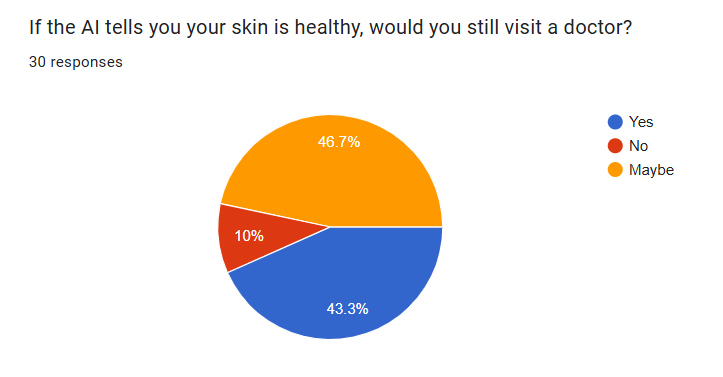
\includegraphics[width=1\linewidth]{trust} 

}

\caption{Survey Response relating to trust}\label{fig:unnamed-chunk-7}
\end{figure}

Notably, 62\% of respondents indicated that they would be more likely to
use the app if it provided \textbf{confidence scores} (e.g., ``85\%
probability of benign mole''). A further 48\% requested \textbf{visual
aids}, such as highlighting the regions of the image that influenced the
prediction. These findings echo growing literature on the importance of
explainable AI in medicine (\citeproc{ref-holzinger2017we}{Holzinger et
al., 2017}).

\begin{figure}[h!]
    \centering
    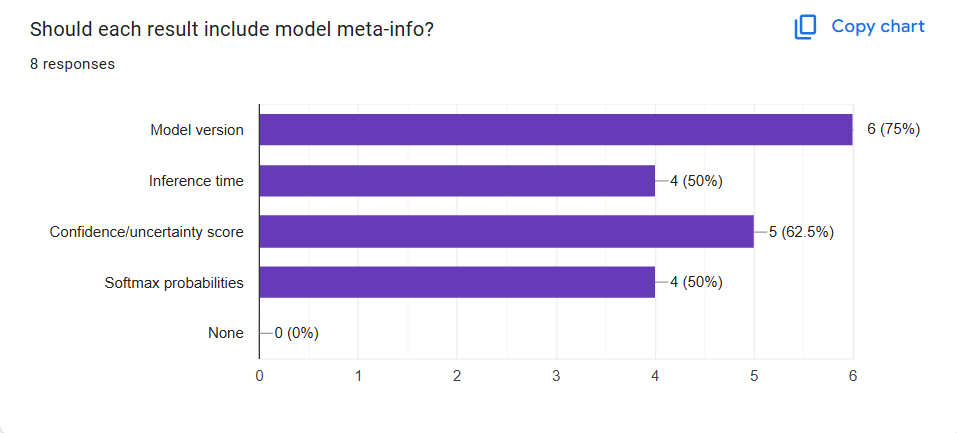
\includegraphics[width=0.45\textwidth]{confidence-score-chart.png}
    \hfill
    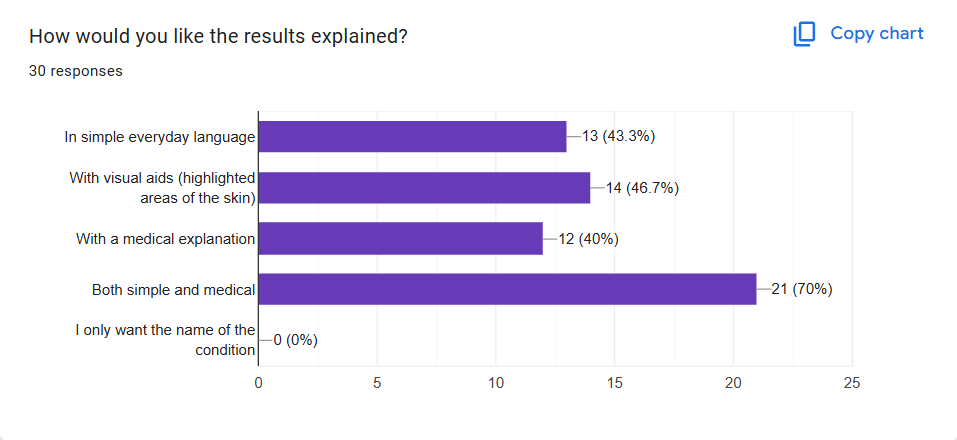
\includegraphics[width=0.45\textwidth]{visual-aids-chart.png}
    \caption{Survey response charts showing demand for confidence score and visual aid in outputs.}
\end{figure}

Trust was also shaped by socio-cultural factors. Respondents from rural
and peri-urban areas were more skeptical of ``invisible'' digital tools
and placed higher value on community healthcare workers or traditional
practices. This highlights the necessity of designing the system not as
a replacement for clinicians, but as a \textbf{support tool} for early
awareness and timely referrals.

\paragraph{Privacy and Data Security
Concerns}\label{privacy-and-data-security-concerns}

Privacy concerns were prominent, with 93\% of respondents expressing at
least some degree of apprehension about uploading personal health
images. The most common fears related to \textbf{data misuse},
\textbf{unauthorized sharing}, and \textbf{inadequate anonymization}.
Younger respondents tended to be more comfortable with data sharing,
provided that transparent consent mechanisms were in place, while older
respondents emphasized the importance of strict confidentiality
policies.

\begin{figure}[h!]
    \centering
    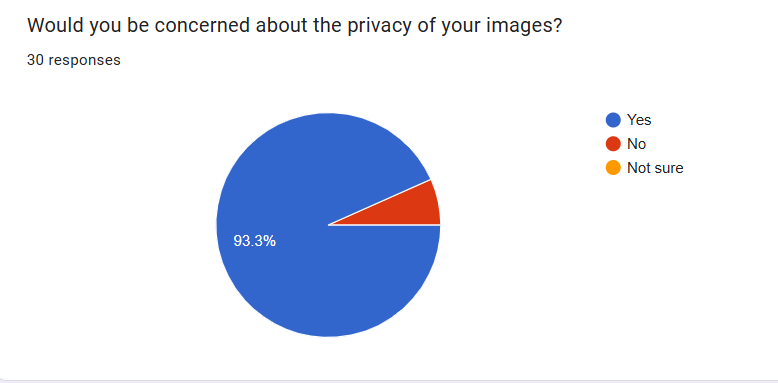
\includegraphics[width=0.45\textwidth]{privacy-chart1.png}
    \hfill
    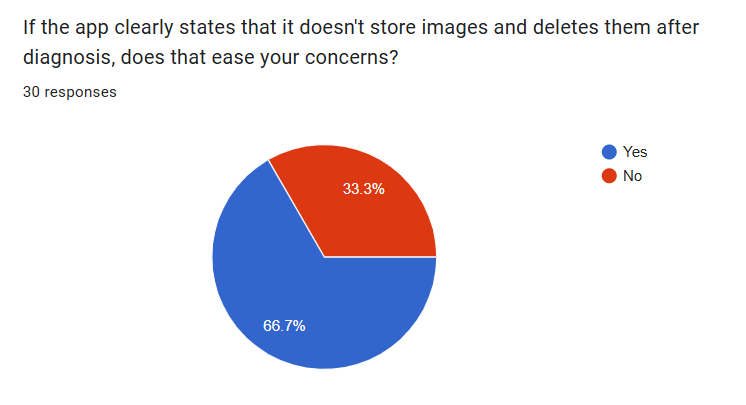
\includegraphics[width=0.45\textwidth]{privacy-chart2.png}
    \caption{Survey response charts showing concerns on privacy.}
\end{figure}

When asked which privacy features they would consider most reassuring,
the following ranked highest:

\begin{enumerate}
\def\labelenumi{\arabic{enumi}.}
\tightlist
\item
  \textbf{On-device processing} -- ensuring images are not uploaded to
  external servers unnecessarily.\\
\item
  \textbf{Data anonymization} -- removing all personally identifiable
  information before processing.\\
\item
  \textbf{Clear terms of use} -- simple, non-technical explanations of
  what happens to user data.
\end{enumerate}

Interestingly, over 66\% indicated they would feel more at ease if the
app was to clearly state that it doesn't save user images after analysis
and predictions. This indicates that privacy is not just an ethical or
regulatory requirement, but also a potential driver of user adoption.

\paragraph{Summary of Insights}\label{summary-of-insights}

The descriptive statistics of general users reveal a population that is
both \textbf{interested in and cautious about} AI in healthcare.
Demographically diverse, the respondents highlight clear generational
and geographic divides in trust, privacy expectations, and feature
preferences. While younger, urban users are more receptive to
experimentation with AI-driven diagnostics, older and rural users
emphasize caution, privacy, and practicality.

These insights carry profound implications for system design:

\begin{itemize}
\tightlist
\item
  The interface must be simple enough for users with limited digital
  literacy.\\
\item
  Privacy and offline processing must be central to design, not
  afterthoughts.\\
\item
  Explainability features (confidence scores, saliency maps) are
  essential for building trust.\\
\item
  Educational content must be embedded to ensure predictions are not
  misinterpreted.
\end{itemize}

Taken together, these findings provide the foundational logic for
designing a mobile health application that is technically sophisticated
yet socially attuned. The next section will shift focus to the
\textbf{technical/professional survey}, where the expectations of
clinicians and researchers are analyzed in greater detail.

\subsubsection{Descriptive Statistics: Technical/Professional
Users}\label{descriptive-statistics-technicalprofessional-users}

The second segment of the survey targeted \textbf{technical and
professional users}, including software developers, engineers, computer
scientists, and healthcare practitioners with some technical exposure
(e.g., laboratory technicians, nurses). This group was of particular
interest because they represent the individuals most likely to engage
directly with the proposed system's backend interfaces, such as the
\textbf{command-line tool (CLI)} or model API. Unlike general users,
these respondents were expected to provide more nuanced insights
regarding \textbf{technical requirements, model transparency,
integration, and workflow compatibility}.

\paragraph{Respondent Demographics and
Roles}\label{respondent-demographics-and-roles}

The professional respondent pool included a diverse set of roles: mobile
application developer, laboratory technician, nursing professional,
computer/software engineers, students in computing-related disciplines,
and computer scientists. This distribution suggests that while the
majority of respondents were \textbf{technically oriented}, there was
also representation from the \textbf{healthcare domain}, ensuring that
perspectives on both medical and technical utility were considered.

\begin{figure}

{\centering 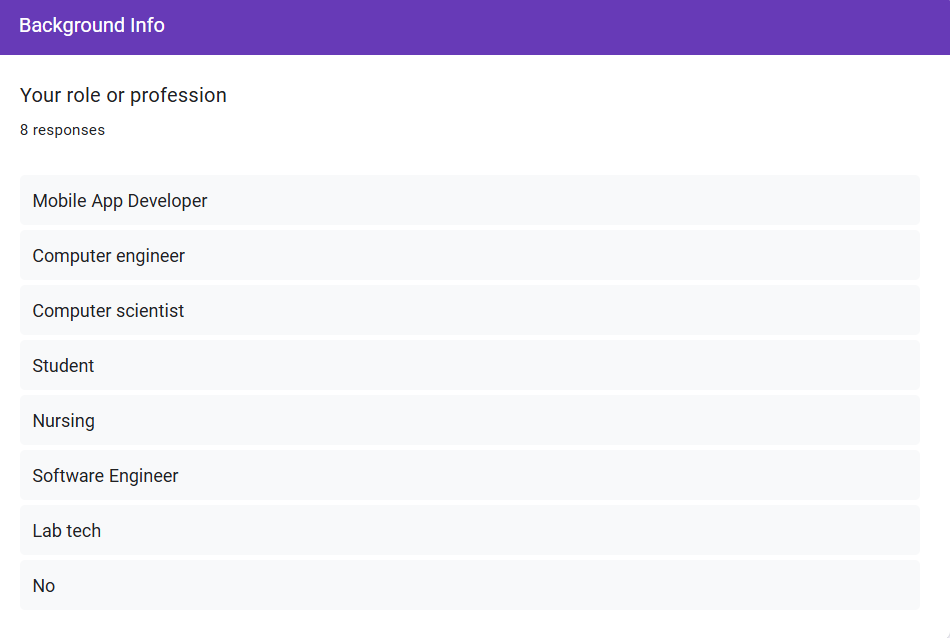
\includegraphics[width=1\linewidth]{technical-user-chart1} 

}

\caption{TDistribution of Respondent Professions}\label{fig:unnamed-chunk-8}
\end{figure}

\paragraph{Experience with Medical
Imaging}\label{experience-with-medical-imaging}

When asked about prior experience with medical imaging or skin lesion
datasets, only a \textbf{small minority (two respondents)} indicated
direct involvement. The vast majority had not previously worked with
medical imaging tasks, underscoring the fact that while these
professionals had strong technical foundations, they were not
necessarily domain specialists. This aligns with similar studies where
developers were found to be technically proficient but often lacked
medical training, highlighting the need for tools that can bridge this
gap (\citeproc{ref-holzinger2017we}{Holzinger et al., 2017}).

\begin{figure}

{\centering 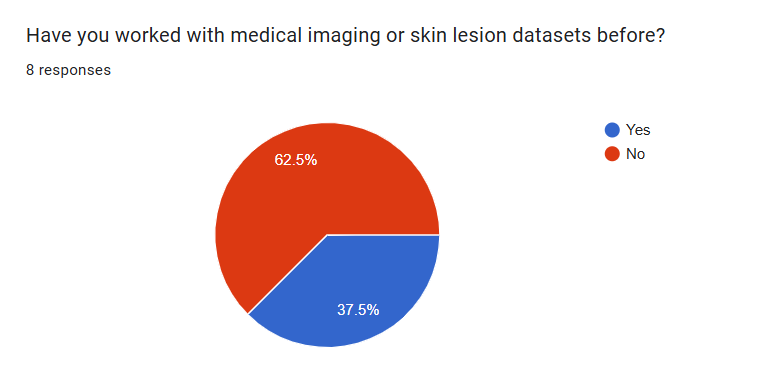
\includegraphics[width=1\linewidth]{technical-user-chart2} 

}

\caption{Prior Experience with Medical Imaging}\label{fig:unnamed-chunk-9}
\end{figure}

\paragraph{Tools and Frameworks Used}\label{tools-and-frameworks-used}

Respondents reported a wide array of tools and frameworks used in their
work. The most common were \textbf{Python and its machine learning
libraries (TensorFlow, PyTorch, Keras)}, often paired with
\textbf{Jupyter Notebook} or \textbf{Google Colab}. Some respondents
mentioned \textbf{MATLAB} for research-oriented tasks, while others in
healthcare roles (e.g., lab technician) leaned towards simpler tools
like \textbf{Excel or Power BI} for reporting and data handling.

This diversity highlights the importance of designing the system with
\textbf{Python-first compatibility}, while ensuring outputs are also
easily exportable to more general tools for broader accessibility.

\begin{figure}

{\centering 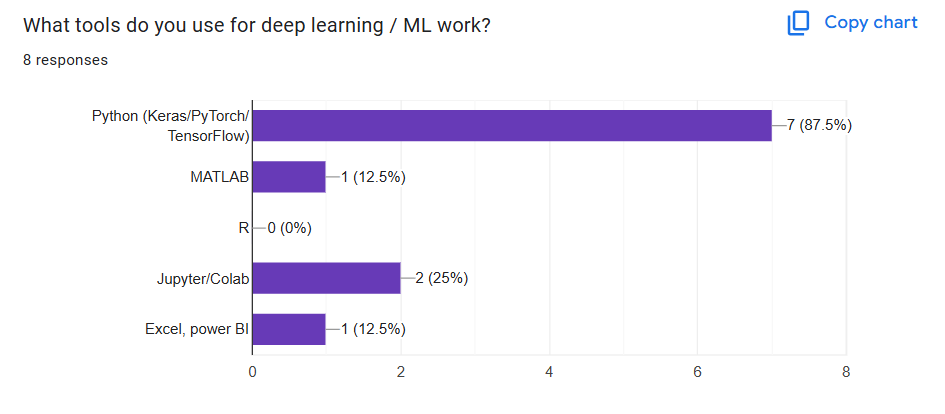
\includegraphics[width=1\linewidth]{technical-user-chart3} 

}

\caption{Tools and Frameworks Used by Respondents}\label{fig:unnamed-chunk-10}
\end{figure}

\paragraph{Usefulness of a CLI Tool}\label{usefulness-of-a-cli-tool}

When asked about the usefulness of a CLI-based system for lesion
detection, the overwhelming majority responded \textbf{positively}. They
viewed the CLI as an essential feature for \textbf{batch analysis,
automation, and research reproducibility}. Only one respondent, a
laboratory technician, expressed reservations, preferring
\textbf{simplified reporting interfaces} instead. This validates the
dual-interface approach of the project: providing both a \textbf{CLI for
professionals} and a \textbf{user-friendly app for general users}.

\begin{figure}

{\centering 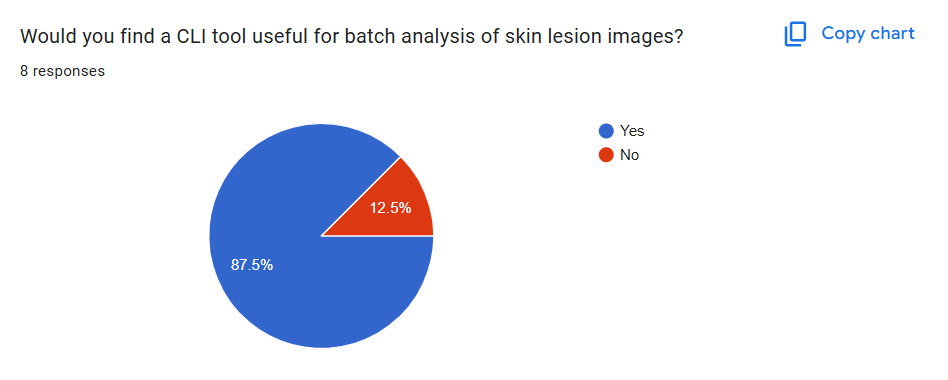
\includegraphics[width=1\linewidth]{technical-user-chart4} 

}

\caption{Perceived Usefulness of CLI}\label{fig:unnamed-chunk-11}
\end{figure}

\paragraph{Preferred Input and Output
Formats}\label{preferred-input-and-output-formats}

Preferences for data input varied but leaned strongly toward
\textbf{directories of images} for batch analysis. Some respondents also
suggested \textbf{zipped archives} or inclusion of \textbf{metadata
files (CSV/JSON)} for organizing annotations.

For output formats, preferences were distributed as follows:

\begin{itemize}
\tightlist
\item
  \textbf{Machine-readable formats}: JSON and CSV were highly favored,
  allowing seamless integration into existing workflows.
\item
  \textbf{Visual overlays}: Several respondents emphasized the
  importance of \textbf{heatmaps (e.g., Grad-CAM)} to highlight lesion
  regions, serving both validation and explainability purposes.
\item
  \textbf{Reports}: A smaller but notable portion highlighted
  \textbf{PDF reports}, particularly relevant to healthcare
  professionals who required clinical-style documentation.
\end{itemize}

This multi-format preference indicates the need for \textbf{flexible
export functionality}, ensuring the system serves both technical and
semi-technical users.

\begin{figure}

{\centering 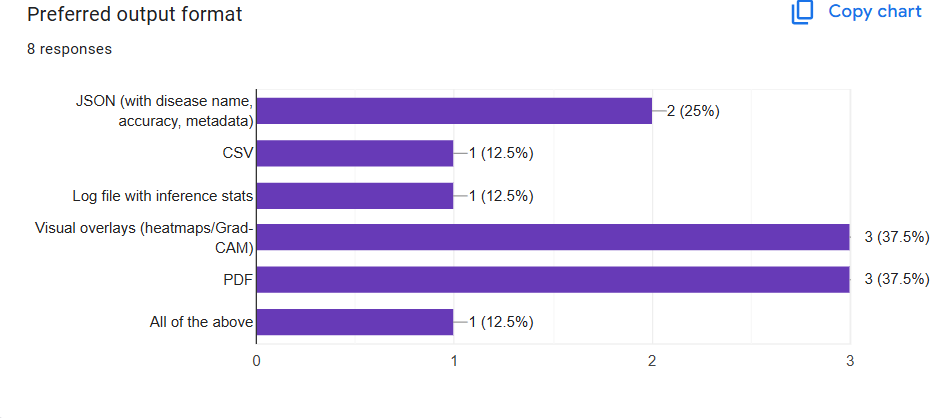
\includegraphics[width=1\linewidth]{technical-user-chart6} 

}

\caption{Preferred Output Formats}\label{fig:unnamed-chunk-12}
\end{figure}

\paragraph{Batch and Asynchronous
Support}\label{batch-and-asynchronous-support}

The majority of technical respondents emphasized the importance of
\textbf{batch or asynchronous support}. They highlighted that
scalability and efficiency are critical in handling large image sets,
especially in research or clinical trial contexts. This aligns with
modern AI system design principles, which prioritize \textbf{parallel
processing} and \textbf{non-blocking workflows}
(\citeproc{ref-lecun2015deep}{LeCun et al., 2015}).

\paragraph{Model Metadata and
Transparency}\label{model-metadata-and-transparency}

Respondents were also asked about the types of metadata they considered
important when generating outputs. The most commonly cited elements
included:

\begin{itemize}
\tightlist
\item
  \textbf{Model version} (to ensure reproducibility)
\item
  \textbf{Inference time} (to assess efficiency)
\item
  \textbf{Confidence or uncertainty scores}
\item
  \textbf{Class probabilities (softmax outputs)}
\end{itemize}

These preferences suggest that technical users prioritize
\textbf{traceability and reliability}, with an expectation that each
prediction is accompanied by sufficient metadata to allow critical
evaluation.

\begin{figure}

{\centering 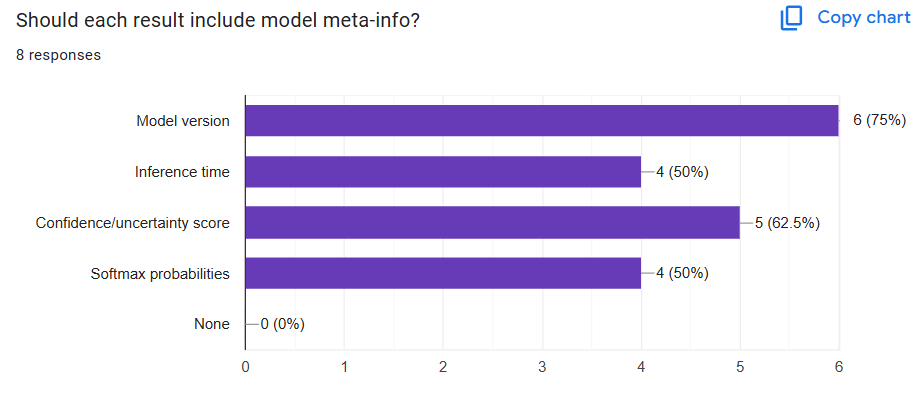
\includegraphics[width=1\linewidth]{technical-user-chart8} 

}

\caption{Desired Model Metadata in Outputs}\label{fig:unnamed-chunk-13}
\end{figure}

\paragraph{Re-training and
Explainability}\label{re-training-and-explainability}

A significant majority expressed interest in the ability to
\textbf{re-train or fine-tune the model} on their own datasets, citing
reasons such as adaptation to specific populations or research domains.
In addition, nearly all respondents highlighted the importance of
\textbf{explainability tools}, particularly \textbf{visual methods like
Grad-CAM or algorithm-agnostic approaches like LIME}, to justify and
contextualize model predictions. This reflects the increasing consensus
in the literature that explainability is essential in medical AI
adoption (\citeproc{ref-doshi2017towards}{Doshi-Velez \& Kim, 2017};
\citeproc{ref-holzinger2017we}{Holzinger et al., 2017}).

\paragraph{Integration Suggestions}\label{integration-suggestions}

Finally, respondents provided several free-text suggestions for
improving integration and usability:

\begin{itemize}
\tightlist
\item
  Support for \textbf{batch and asynchronous execution}.
\item
  Integration of \textbf{feedback loops} to continuously improve the
  model over time.
\item
  Development of \textbf{dashboards or lightweight web interfaces}
  layered on top of the CLI for hybrid users.
\end{itemize}

Collectively, these recommendations underscore the \textbf{dual
necessity of technical depth and user accessibility}, which is
consistent with best practices in designing medical AI systems
(\citeproc{ref-ventola2014mobile}{Ventola, 2014}).

\paragraph{Summary}\label{summary-1}

In summary, the technical and professional survey respondents
demonstrated a strong demand for \textbf{flexibility, scalability,
transparency, and explainability}. While most lacked direct medical
imaging experience, their technical expertise positioned them as key
stakeholders in shaping the system's \textbf{backend design and advanced
features}. Their responses highlight the need for a system that is
simultaneously \textbf{Python-integrated, CLI-compatible, metadata-rich,
and explainable}, with sufficient support for both
\textbf{machine-readable and human-readable outputs}.

\subsubsection{Cross-Survey Comparative
Insights}\label{cross-survey-comparative-insights}

This section synthesizes findings from both the general user survey and
the technical/professional user survey. It highlights areas where
perspectives converge, where they diverge, and the implications these
patterns hold for system requirements.

\paragraph{Points of Convergence (Shared Concerns and
Priorities)}\label{points-of-convergence-shared-concerns-and-priorities}

Across both general users (non-technical) and technical/professional
users, several common themes emerged:

\begin{enumerate}
\def\labelenumi{\arabic{enumi}.}
\item
  \textbf{Desire for Accurate and Trustworthy Predictions:}\\
  Both groups emphasized that diagnostic reliability was paramount.
  Users---technical or not---wanted confidence scores or probabilities
  to be reported.
\item
  \textbf{Importance of Explainability:}\\
  While technical respondents explicitly mentioned interpretability
  methods such as Grad-CAM and LIME, general users also stressed the
  need for clear explanations in plain language. This highlights a
  shared demand for transparency, albeit at different levels of
  technical detail.
\item
  \textbf{User-Centric Outputs:}\\
  Both groups valued outputs that could be used beyond the app itself.

  \begin{itemize}
  \tightlist
  \item
    General users preferred simple, readable summaries they could share
    with doctors.\\
  \item
    Technical users preferred structured outputs (e.g., JSON, CSV,
    visual overlays) that could feed into research workflows.\\
    Ultimately, both groups wanted portability and shareability of
    results.
  \end{itemize}
\item
  \textbf{Scalability Expectations:}\\
  General users asked for responsiveness under high load (e.g., fast
  results even with weak connectivity).\\
  Technical users demanded batch processing and asynchronous
  execution.\\
  Together, this suggests that system performance under varying usage
  scenarios is a universal requirement.
\end{enumerate}

\paragraph{Divergences Between User
Groups}\label{divergences-between-user-groups}

Despite these convergences, important divergences were observed:

\begin{enumerate}
\def\labelenumi{\arabic{enumi}.}
\item
  \textbf{Interface Expectations:}

  \begin{itemize}
  \tightlist
  \item
    General users overwhelmingly preferred a mobile application with a
    graphical interface, prioritizing ease of use and minimal technical
    barriers.\\
  \item
    Technical users favored a command-line interface (CLI) that
    supported automation, scripting, and integration into research
    pipelines.
  \end{itemize}
\item
  \textbf{Depth of Metadata and Reporting:}

  \begin{itemize}
  \tightlist
  \item
    General users were primarily interested in basic predictions and
    clinic recommendations.\\
  \item
    Technical users demanded detailed metadata: model version, inference
    latency, softmax scores, dataset provenance, and uncertainty
    measures.
  \end{itemize}
\item
  \textbf{Re-training and Customization:}

  \begin{itemize}
  \tightlist
  \item
    General users had little to no concern with re-training models.\\
  \item
    Technical respondents strongly favored the ability to fine-tune
    models with their own datasets.
  \end{itemize}
\item
  \textbf{Explainability Format:}

  \begin{itemize}
  \tightlist
  \item
    General users wanted plain-text, user-friendly explanations
    supplemented with visuals if needed.\\
  \item
    Technical users sought deep interpretability techniques like
    heatmaps, decision trees, and statistical confidence intervals.
  \end{itemize}
\item
  \textbf{Data Input Modes:}

  \begin{itemize}
  \tightlist
  \item
    General users imagined simply uploading an image.\\
  \item
    Technical users wanted flexibility: batch image folders, CSV
    metadata, JSON, and zip file uploads.
  \end{itemize}
\end{enumerate}

\paragraph{Implications for System
Requirements}\label{implications-for-system-requirements}

From these convergences and divergences, several key implications for
system design emerge:

\begin{enumerate}
\def\labelenumi{\arabic{enumi}.}
\item
  \textbf{Dual-Interface Strategy:}

  \begin{itemize}
  \tightlist
  \item
    A mobile app should cater to general users, prioritizing simplicity,
    readability, and clinic-focused usability.\\
  \item
    A CLI should be built for technical users, prioritizing flexibility,
    batch processing, detailed outputs, and integration into research
    workflows.
  \end{itemize}
\item
  \textbf{Tiered Explainability:} The system must deliver different
  layers of explanation:

  \begin{itemize}
  \tightlist
  \item
    Plain-language summaries for laypersons.\\
  \item
    Heatmaps, metadata, and statistical insights for professionals.
  \end{itemize}
\item
  \textbf{Multi-Format Output Support:}\\
  Both machine-readable (JSON, CSV) and human-readable (PDF, summary
  reports) outputs must be supported. This dual approach ensures
  usability across the spectrum of end-users.
\item
  \textbf{Performance and Scalability}\\
  Responsiveness must be optimized not just for individual mobile users,
  but also for batch research workloads. This likely necessitates
  cloud-based infrastructure with both synchronous (real-time) and
  asynchronous (background job) processing modes.
\item
  \textbf{Customizability for Professionals}\\
  To serve the research community, the CLI must allow optional
  re-training or fine-tuning, as well as dataset re-use. This is
  unnecessary for general users but critical for adoption among
  professionals.
\end{enumerate}

\subsection{System Overview}\label{system-overview}

This section presents a high-level overview of the proposed Skin Lesion
Detection and Classification System. It begins by clarifying the
system's objectives, followed by identifying the intended users and
stakeholders. The section then outlines the boundaries and scope of the
system and finally highlights the key functionalities at a high level.

\subsubsection{Objectives of the Proposed
System}\label{objectives-of-the-proposed-system}

The overarching goal of the proposed system is to provide an effective,
accessible, and scientifically robust tool for the detection and
classification of skin lesions. In particular, the objectives include:

\begin{enumerate}
\def\labelenumi{\arabic{enumi}.}
\item
  \textbf{Facilitating Early Detection of Skin Conditions}\\
  By enabling individuals to take or upload images of skin lesions and
  receive automated classification, the system promotes early
  identification of potentially malignant conditions, which is crucial
  for timely medical intervention.
\item
  \textbf{Providing Decision Support to Health Professionals}\\
  The system is designed not to replace dermatologists but to augment
  their diagnostic process by providing rapid and accurate
  pre-screening. This decision-support function is particularly
  beneficial in resource-limited settings.
\item
  \textbf{Improving Accessibility of Dermatological Insights}\\
  Through a mobile interface, the system brings dermatological
  assessment closer to populations with limited access to healthcare
  facilities. It democratizes diagnostic insights beyond specialized
  clinics.
\item
  \textbf{Supporting Research and Development}\\
  By offering a CLI that supports batch processing, detailed output, and
  dataset integration, the system also serves the academic and clinical
  research community. This ensures that the system is not only a
  public-facing tool but also a research-grade infrastructure.
\item
  \textbf{Balancing Accuracy with Explainability}\\
  The system will incorporate interpretable machine learning methods to
  explain classifications in both layman-friendly and professional
  detail. This addresses the dual concerns of trust and transparency.
\end{enumerate}

\subsubsection{Target Users and
Stakeholders}\label{target-users-and-stakeholders}

The system is targeted at two distinct yet complementary user groups,
alongside several key stakeholders:

\begin{enumerate}
\def\labelenumi{\arabic{enumi}.}
\item
  \textbf{General Users (Patients and Care Seekers):}

  \begin{itemize}
  \tightlist
  \item
    Non-technical individuals who will primarily access the system
    through a mobile app.\\
  \item
    Require a simple workflow: upload an image, receive a
    classification, and obtain understandable recommendations.\\
  \item
    Value ease of use, speed, and actionable next steps (e.g., advice to
    visit a dermatologist).
  \end{itemize}
\item
  \textbf{Health Professionals and Researchers:}

  \begin{itemize}
  \tightlist
  \item
    Dermatologists, clinicians, and biomedical researchers who will
    primarily interact via a command-line interface (CLI).\\
  \item
    Require detailed outputs such as confidence scores, batch
    processing, integration with existing datasets, and
    reproducibility.\\
  \item
    May use the system as a teaching tool, research aid, or diagnostic
    support mechanism.
  \end{itemize}
\item
  \textbf{Key Stakeholders:}

  \begin{itemize}
  \tightlist
  \item
    \textbf{Healthcare Institutions:} Benefit from reduced workload in
    screening and triaging.\\
  \item
    \textbf{Policy Makers and NGOs:} Gain from public health insights,
    particularly in regions where skin cancer screening is rare.\\
  \item
    \textbf{Technical Developers and Maintainers:} Ensure continuous
    improvement, reliability, and deployment.\\
  \item
    \textbf{Academic Community:} Uses system outputs for dermatology and
    machine learning research.
  \end{itemize}
\end{enumerate}

\subsubsection{System Boundaries and
Scope}\label{system-boundaries-and-scope}

The boundaries and scope of the system are clearly defined to avoid
overextension and maintain focus:

\begin{itemize}
\item
  \textbf{In-Scope Features:}

  \begin{itemize}
  \tightlist
  \item
    Classification of skin lesion images into predefined categories
    (e.g., benign vs malignant, or further into multiple classes
    depending on dataset).\\
  \item
    Confidence reporting and explanation generation.\\
  \item
    Two interfaces: mobile application for general users, CLI for
    technical users.\\
  \item
    Secure communication with a backend inference API.\\
  \item
    Limited offline functionality (basic inference on-device possible,
    with cloud fallback for heavy processing).\\
  \item
    Support for continuous updates and improvements via retraining
    mechanisms (primarily CLI-driven).
  \end{itemize}
\item
  \textbf{Out-of-Scope Features:}

  \begin{itemize}
  \tightlist
  \item
    Direct integration with electronic health records (EHR) systems at
    this stage.\\
  \item
    Automated treatment recommendations beyond advising a medical
    consultation.\\
  \item
    Full offline deployment for all users, as this may be infeasible on
    low-end devices.\\
  \item
    Non-dermatological conditions (focus is strictly skin lesions).
  \end{itemize}
\end{itemize}

\subsubsection{High-Level
Functionalities}\label{high-level-functionalities}

At a high level, the proposed system will provide the following
functionalities:

\begin{enumerate}
\def\labelenumi{\arabic{enumi}.}
\item
  \textbf{Image Input and Preprocessing:}

  \begin{itemize}
  \tightlist
  \item
    Mobile: Single image capture or upload.\\
  \item
    CLI: Single image, folder batch, or dataset file.
  \end{itemize}
\item
  \textbf{Automated Lesion Classification:}

  \begin{itemize}
  \tightlist
  \item
    Inference performed by a trained CNN model (ResNet-based).\\
  \item
    Output includes predicted class, confidence score, and alternative
    predictions.
  \end{itemize}
\item
  \textbf{Explainability and Interpretability:}

  \begin{itemize}
  \tightlist
  \item
    Mobile: Simplified plain-language explanation plus optional
    heatmap.\\
  \item
    CLI: Detailed interpretability (e.g., Grad-CAM, numerical feature
    attribution).
  \end{itemize}
\item
  \textbf{Result Delivery:}

  \begin{itemize}
  \tightlist
  \item
    Mobile: Readable on-screen summary with option to save or share
    report (e.g., PDF).\\
  \item
    CLI: Structured output formats (CSV, JSON, PDF).
  \end{itemize}
\item
  \textbf{Continuous Improvement Loop:}

  \begin{itemize}
  \tightlist
  \item
    Mechanisms for incorporating user feedback.\\
  \item
    Optional retraining capabilities for researchers using CLI.\\
  \item
    Backend logging of usage patterns (with privacy safeguards) for
    model refinement.
  \end{itemize}
\item
  \textbf{Security and Privacy Safeguards:}

  \begin{itemize}
  \tightlist
  \item
    Anonymization of images and metadata.\\
  \item
    Secure transmission and storage with encryption.\\
  \item
    Compliance with ethical standards regarding sensitive health data.
  \end{itemize}
\end{enumerate}

In summary, this system is envisioned as a dual-purpose platform:
\textbf{a patient-facing mobile app for accessibility and early
detection, and a research-grade CLI for scientific rigor and
extensibility.}

\subsection{Functional Requirements
Analysis}\label{functional-requirements-analysis}

The functional requirements of the system capture the essential features
and capabilities that the application must provide to its diverse set of
users and stakeholders. These requirements are organized into three
categories: \textbf{user-oriented}, \textbf{system-oriented}, and
\textbf{non-functional} requirements. This categorization ensures that
both human-centered needs and technical imperatives are addressed
systematically.

\subsubsection{User-Oriented
Requirements}\label{user-oriented-requirements}

User-oriented requirements describe how the system should interact with
its primary audiences, that is general users and health
professionals/researchers. These requirements ensure that the system
delivers tailored functionality that aligns with the expectations and
technical proficiency of each group.

\paragraph{General Users (Mobile
Application)}\label{general-users-mobile-application}

\begin{enumerate}
\def\labelenumi{\arabic{enumi}.}
\item
  \textbf{Image Capture and Upload}

  \begin{itemize}
  \tightlist
  \item
    The system must allow users to capture lesion images via the device
    camera or upload existing images from the gallery.\\
  \item
    Support for basic cropping and quality-checking prior to submission.
  \end{itemize}
\item
  \textbf{Instant Classification and Feedback}

  \begin{itemize}
  \tightlist
  \item
    After submission, the user should receive the predicted lesion type
    with a confidence score.\\
  \item
    Explanations must be provided in simple, non-technical language.
  \end{itemize}
\item
  \textbf{Health Guidance}

  \begin{itemize}
  \item
    Beyond classification, users should receive actionable suggestions
    such as:

    \begin{itemize}
    \tightlist
    \item
      ``Consult a dermatologist immediately'' (for suspicious
      lesions).\\
    \item
      ``Monitor regularly'' (for benign lesions).
    \end{itemize}
  \item
    The system must not provide treatment instructions beyond suggesting
    professional consultation.
  \end{itemize}
\item
  \textbf{Report Generation and History}

  \begin{itemize}
  \tightlist
  \item
    Users should be able to save results in a report format (e.g., PDF)
    or maintain a personal history log within the application.\\
  \item
    Results history should be accessible in an easy-to-navigate
    interface.
  \end{itemize}
\item
  \textbf{Notifications and Reminders}

  \begin{itemize}
  \tightlist
  \item
    Optional notifications should remind users to recheck lesions at
    specified intervals.\\
  \item
    Users must have full control to enable or disable reminders.
  \end{itemize}
\item
  \textbf{Privacy and Security Assurance}

  \begin{itemize}
  \tightlist
  \item
    The system must anonymize uploaded images and avoid linking them
    with personally identifiable information.
  \end{itemize}
\end{enumerate}

\paragraph{Health Professionals and Researchers
(CLI)}\label{health-professionals-and-researchers-cli}

\begin{enumerate}
\def\labelenumi{\arabic{enumi}.}
\item
  \textbf{Batch Processing Capabilities}

  \begin{itemize}
  \tightlist
  \item
    The CLI must support processing of multiple images or datasets in
    one run.\\
  \item
    Input should accept file paths, directories, or structured dataset
    references.
  \end{itemize}
\item
  \textbf{Detailed Classification Outputs}

  \begin{itemize}
  \tightlist
  \item
    Results should include prediction probabilities for all possible
    classes, not only the top class.\\
  \item
    Outputs should include visual overlays such as Grad-CAM heatmaps
    when requested.
  \end{itemize}
\item
  \textbf{Flexible Output Formats}

  \begin{itemize}
  \tightlist
  \item
    Results must be exportable in CSV, JSON, PDF, or image overlay
    formats.\\
  \item
    Researchers should be able to configure output granularity.
  \end{itemize}
\item
  \textbf{Integration with External Workflows}

  \begin{itemize}
  \tightlist
  \item
    CLI outputs must be scriptable and pipeline-friendly for integration
    with other tools (e.g., data analysis software).
  \end{itemize}
\item
  \textbf{Reproducibility Support}

  \begin{itemize}
  \tightlist
  \item
    The system should log model versions, configuration parameters, and
    dataset references to ensure reproducibility of results.
  \end{itemize}
\item
  \textbf{Extended Explainability Features}

  \begin{itemize}
  \tightlist
  \item
    Provide multiple explanation modalities (numerical feature
    importance, saliency maps, etc.) suitable for academic publications
    or clinical reviews.
  \end{itemize}
\end{enumerate}

\begin{figure}

{\centering 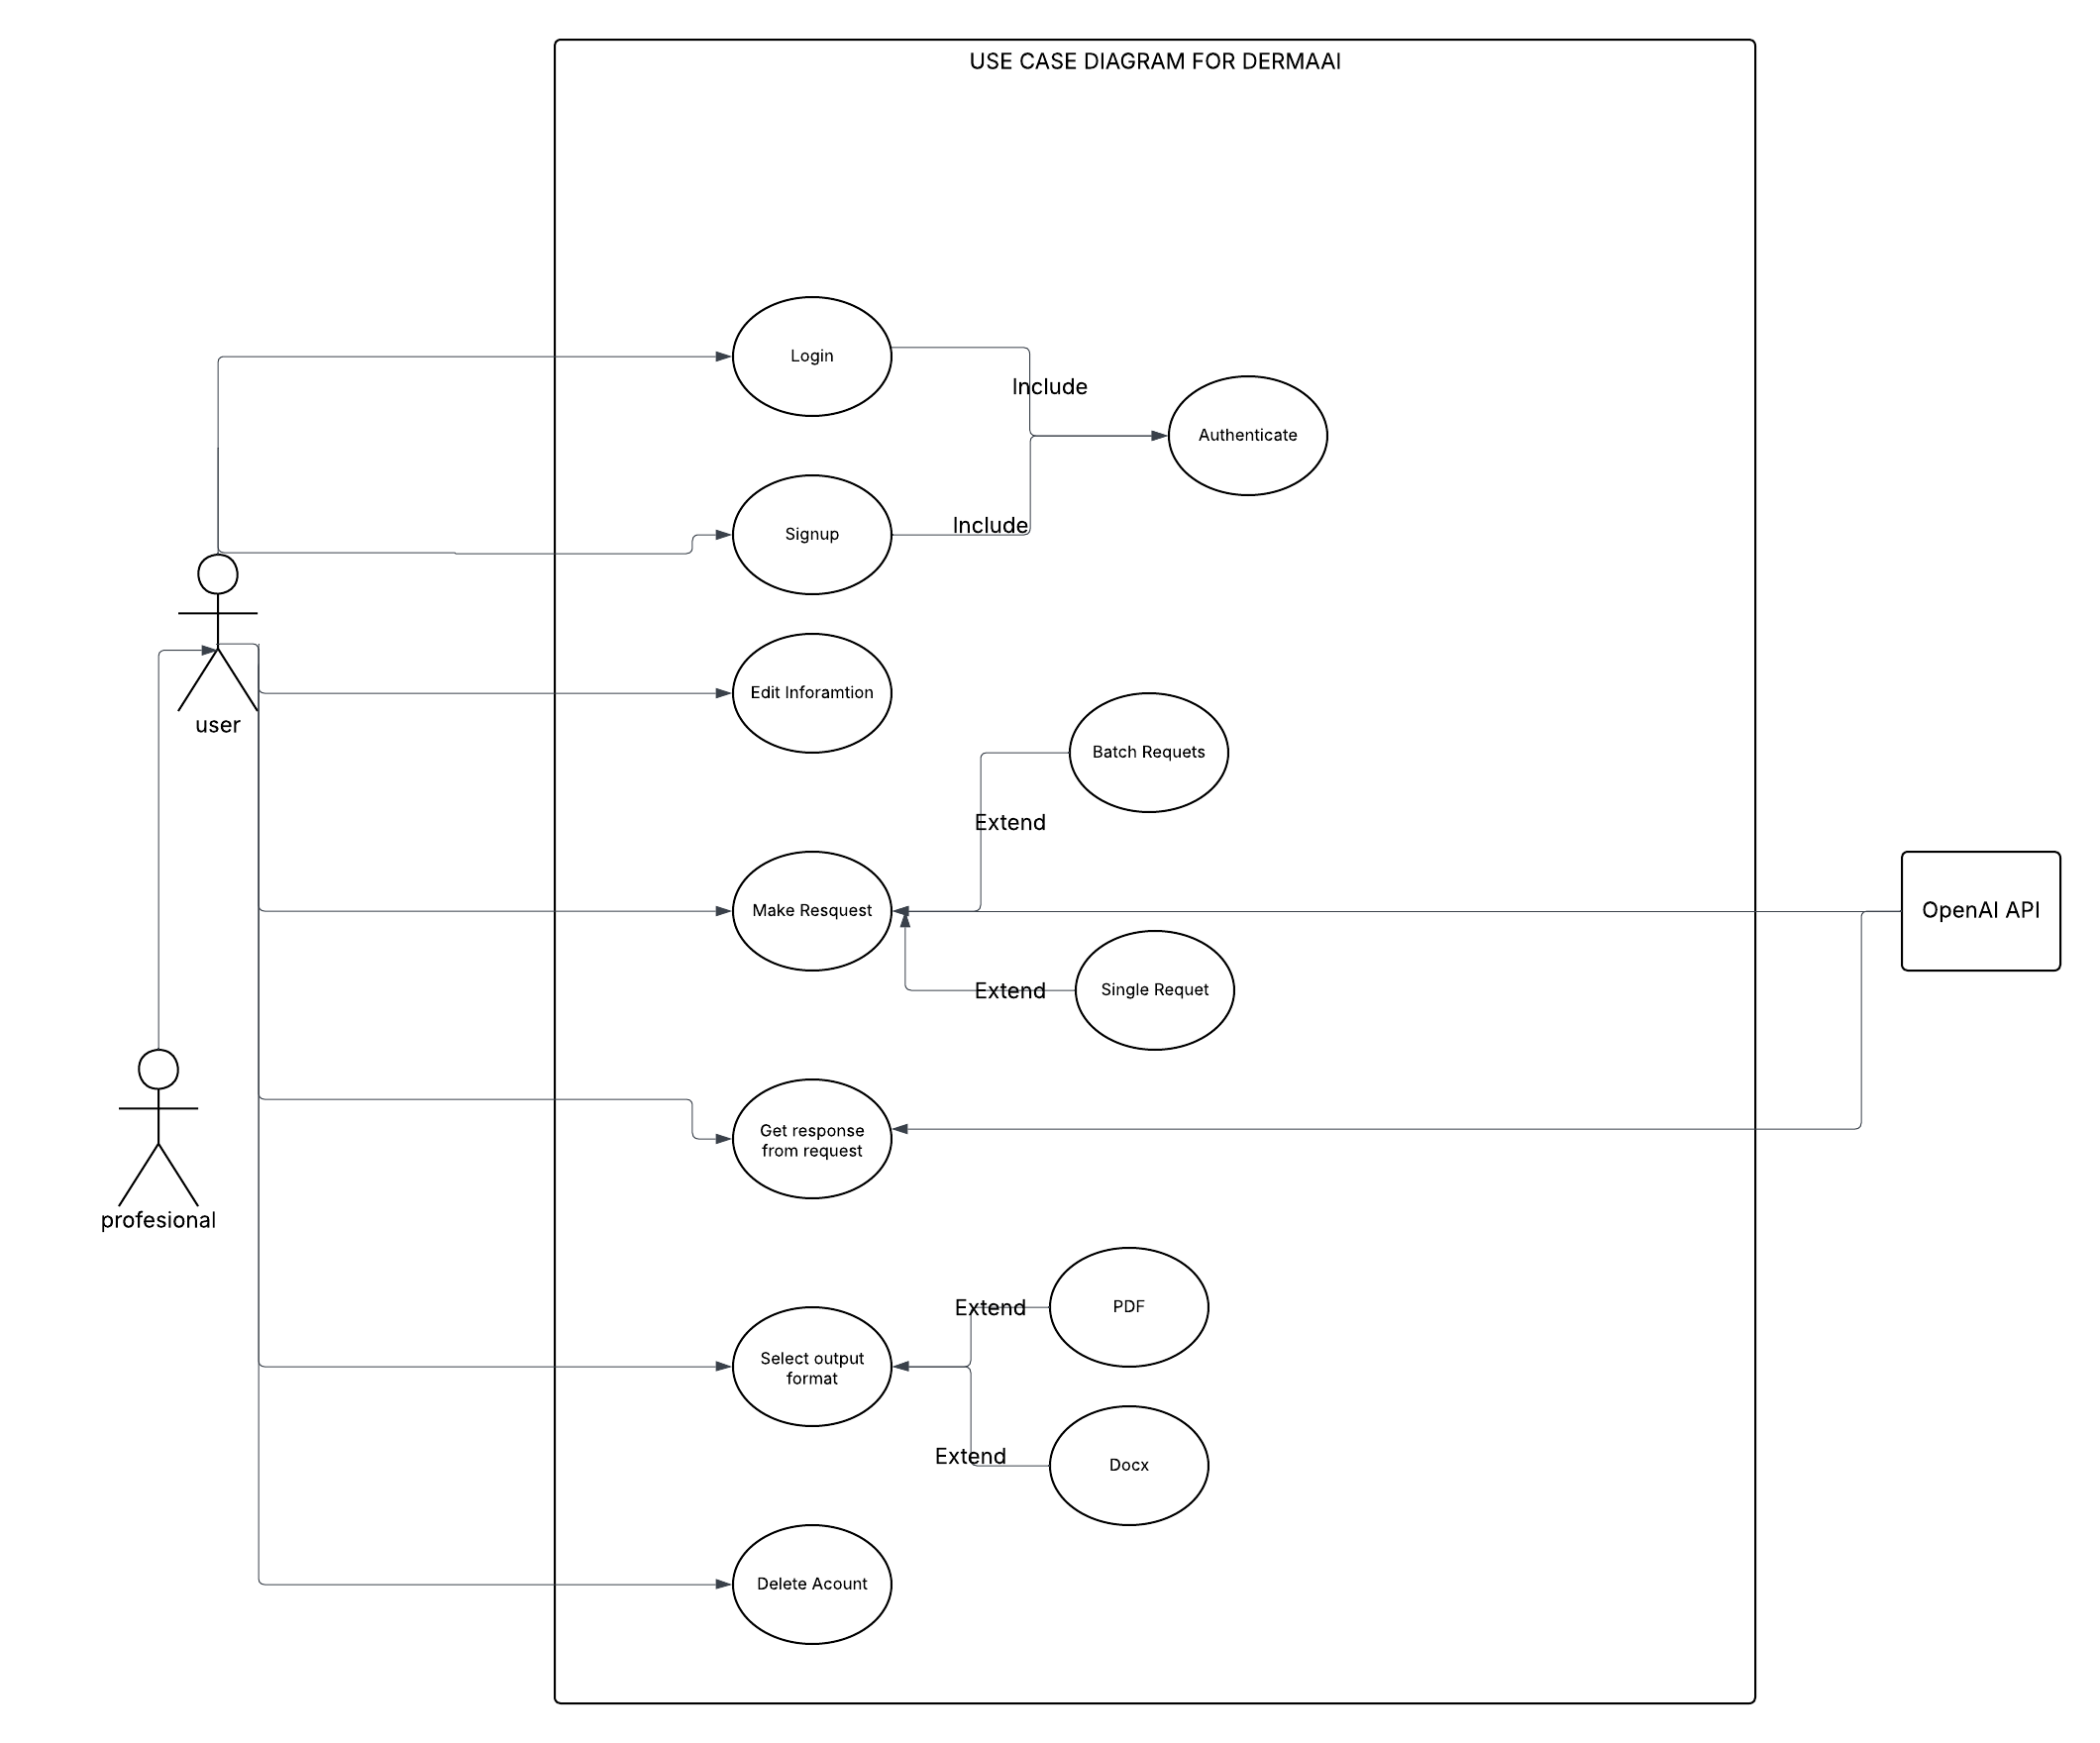
\includegraphics[width=1\linewidth]{DermaAI-Usecase} 

}

\caption{Usecase Diagram for DermaAI}\label{fig:unnamed-chunk-14}
\end{figure}

\subsubsection{System-Oriented
Requirements}\label{system-oriented-requirements}

These requirements define how the system must behave at a technical
level to fulfill user needs effectively.

\paragraph{Model Training and
Inference}\label{model-training-and-inference}

\begin{itemize}
\tightlist
\item
  The system must rely on a CNN (e.g., ResNet-18) trained on a large,
  labeled dataset of skin lesion images.\\
\item
  Training must support transfer learning and fine-tuning to improve
  accuracy.\\
\item
  The inference pipeline must be lightweight enough for deployment in
  mobile and cloud environments.\\
\item
  Support for retraining or fine-tuning must be included for CLI
  researchers.
\end{itemize}

\paragraph{API Communication}\label{api-communication}

\begin{itemize}
\tightlist
\item
  The mobile application must communicate with the inference server
  through secure APIs.\\
\item
  The API must accept inputs (image + optional metadata), run inference,
  and return structured results.\\
\item
  The API must support JSON-based request/response formatting.\\
\item
  Latency should be optimized to provide near real-time results for
  mobile users.
\end{itemize}

\paragraph{Data Handling and Security}\label{data-handling-and-security}

\begin{itemize}
\tightlist
\item
  All uploaded data must be encrypted in transit (TLS) and at rest.\\
\item
  Sensitive information must be anonymized to ensure compliance with
  ethical and legal standards (e.g., GDPR-like principles).\\
\item
  The system must implement secure access controls to prevent
  unauthorized use of the API or model.
\end{itemize}

\subsubsection{Non-Functional
Requirements}\label{non-functional-requirements}

Non-functional requirements define the quality attributes of the system,
ensuring robustness, trustworthiness, and long-term sustainability.

\paragraph{Performance and Accuracy}\label{performance-and-accuracy}

\begin{itemize}
\tightlist
\item
  The system must achieve a minimum accuracy benchmark comparable to
  dermatologists (e.g., ≥85\% for malignant vs.~benign classification as
  in (\citeproc{ref-haenssle2018man}{Haenssle et al., 2018})).\\
\item
  Mobile inference should return results within 5--10 seconds under
  average connectivity conditions.\\
\item
  CLI batch processing should handle at least 1,000 images without
  significant performance degradation.
\end{itemize}

\paragraph{Privacy and Security}\label{privacy-and-security}

\begin{itemize}
\tightlist
\item
  All images must be processed anonymously, with no linkage to personal
  identifiers.\\
\item
  Strong encryption must be enforced for both transmission and
  storage.\\
\item
  The mobile app must allow users to delete stored history at any time.
\end{itemize}

\paragraph{Usability and
Accessibility}\label{usability-and-accessibility}

\begin{itemize}
\tightlist
\item
  The mobile interface must be intuitive, requiring minimal user
  training.\\
\item
  Instructions, labels, and explanations must be provided in clear,
  non-technical language.\\
\item
  Accessibility features such as support for larger fonts, screen
  readers
\end{itemize}

\paragraph{Scalability and
Maintainability}\label{scalability-and-maintainability}

\begin{itemize}
\tightlist
\item
  The backend infrastructure must support horizontal scaling through
  containerization and load balancing.\\
\item
  Modular design must ensure easy updates to models, APIs, and
  interfaces.\\
\item
  Documentation and versioning must be maintained for both mobile and
  CLI components.
\end{itemize}

In summary, the functional requirements establish the foundation of the
proposed system, ensuring that it satisfies the practical needs of its
two core user groups while adhering to strict technical, ethical, and
quality standards.

\subsection{System Architecture}\label{system-architecture}

The proposed skin lesion detection and classification system adopts a
\textbf{serverless, modular architecture} designed for scalability,
cost-efficiency, and seamless integration of advanced AI models. The
system is primarily built upon cloud-native components (Amazon Web
Services) to ensure elasticity and fault tolerance, while remaining
lightweight enough to accommodate future hybrid deployments. Figure 18
(below) illustrates the \textbf{overall serverless architecture of
DermaAI}, integrating both model inference and large language model
(LLM)-based explanation generation.

\begin{figure}

{\centering 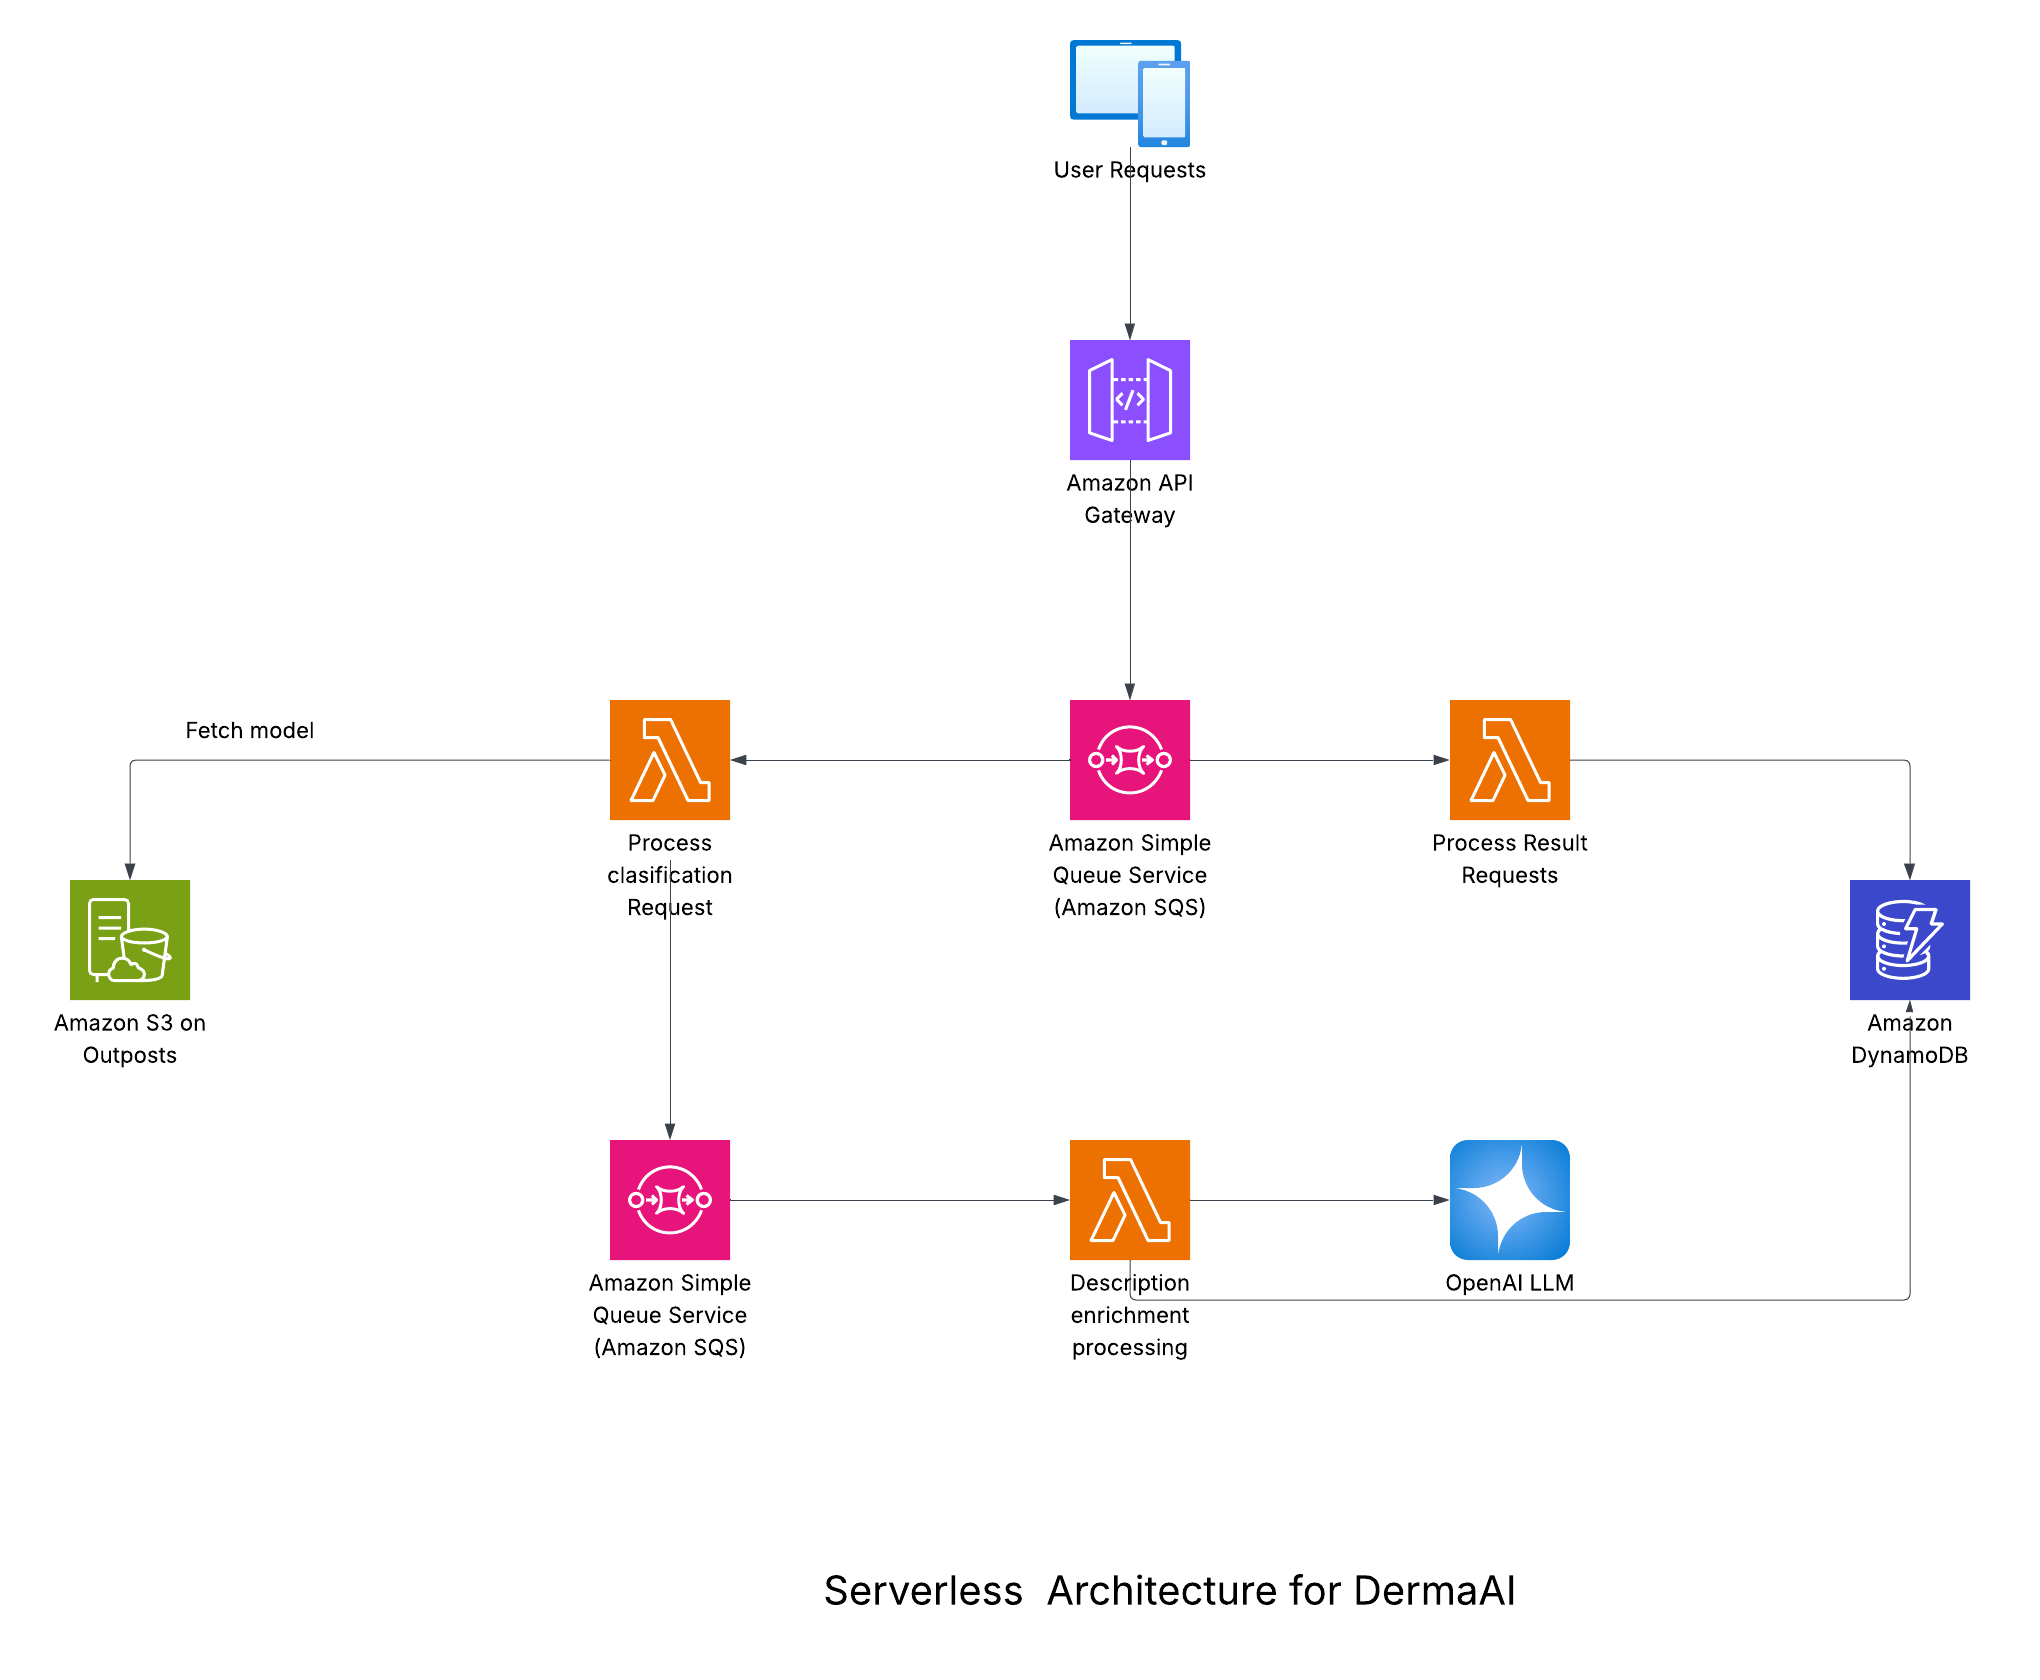
\includegraphics[width=0.5\linewidth]{DermaAI-Architecture} 

}

\caption{Serverless Architecture for DermaAI}\label{fig:unnamed-chunk-15}
\end{figure}

At a high level, the system architecture can be broken down into the
following core components:

\begin{enumerate}
\def\labelenumi{\arabic{enumi}.}
\item
  \textbf{User Interaction Layer (Clients)}\\
  Users, whether through a mobile application or a command-line
  interface (CLI), initiate requests by uploading an image of a skin
  lesion along with optional metadata. This forms the primary entry
  point into the system.
\item
  \textbf{API Gateway}\\
  All requests are routed through \textbf{Amazon API Gateway}, which
  standardizes inputs, enforces request validation, and provides an
  interface for secure communication between clients and backend
  services. It also supports monitoring and throttling, ensuring the
  system can scale gracefully under heavy load.
\item
  \textbf{Queue Management (Amazon SQS)}\\
  Requests are decoupled and passed into \textbf{Amazon Simple Queue
  Service (SQS)} for asynchronous processing. This design ensures that
  bursts of user activity do not overwhelm the backend, while also
  supporting fault tolerance and retries.
\item
  \textbf{Model Inference Layer}\\
  A dedicated \textbf{AWS Lambda function} fetches the pretrained CNN
  model (stored in \textbf{Amazon S3}) and processes the classification
  request. This serverless function performs \textbf{image
  preprocessing, model inference, and preliminary result formatting}.
\item
  \textbf{Result Enrichment Layer (LLM Integration)}\\
  To provide contextually rich, human-friendly explanations, another
  \textbf{Lambda function} triggers communication with the
  \textbf{OpenAI LLM}. This step enhances the raw model predictions with
  medically accurate, user-friendly descriptions, usage guidelines, and
  disclaimers.
\item
  \textbf{Data Storage and Retrieval}\\
  The system employs \textbf{Amazon DynamoDB} for storing user requests,
  model outputs, enriched explanations, and metadata. This NoSQL storage
  ensures fast queries for both individual lookups (e.g., retrieving a
  patient's history) and analytical queries for research purposes.
\item
  \textbf{Feedback Loop and Continuous Improvement}\\
  User interactions and outcomes are logged into DynamoDB, forming the
  basis for continuous model evaluation. This feedback mechanism enables
  future retraining of the CNN model and refinement of the LLM prompts.
\end{enumerate}

\subsubsection{Model Architecture}\label{model-architecture-1}

At the core of the system lies a \textbf{Convolutional Neural Network
(CNN)}, fine-tuned from a pretrained ResNet18 backbone. This
architecture was chosen due to its proven efficiency in medical image
classification tasks, balancing computational cost with diagnostic
accuracy.

\begin{figure}

{\centering 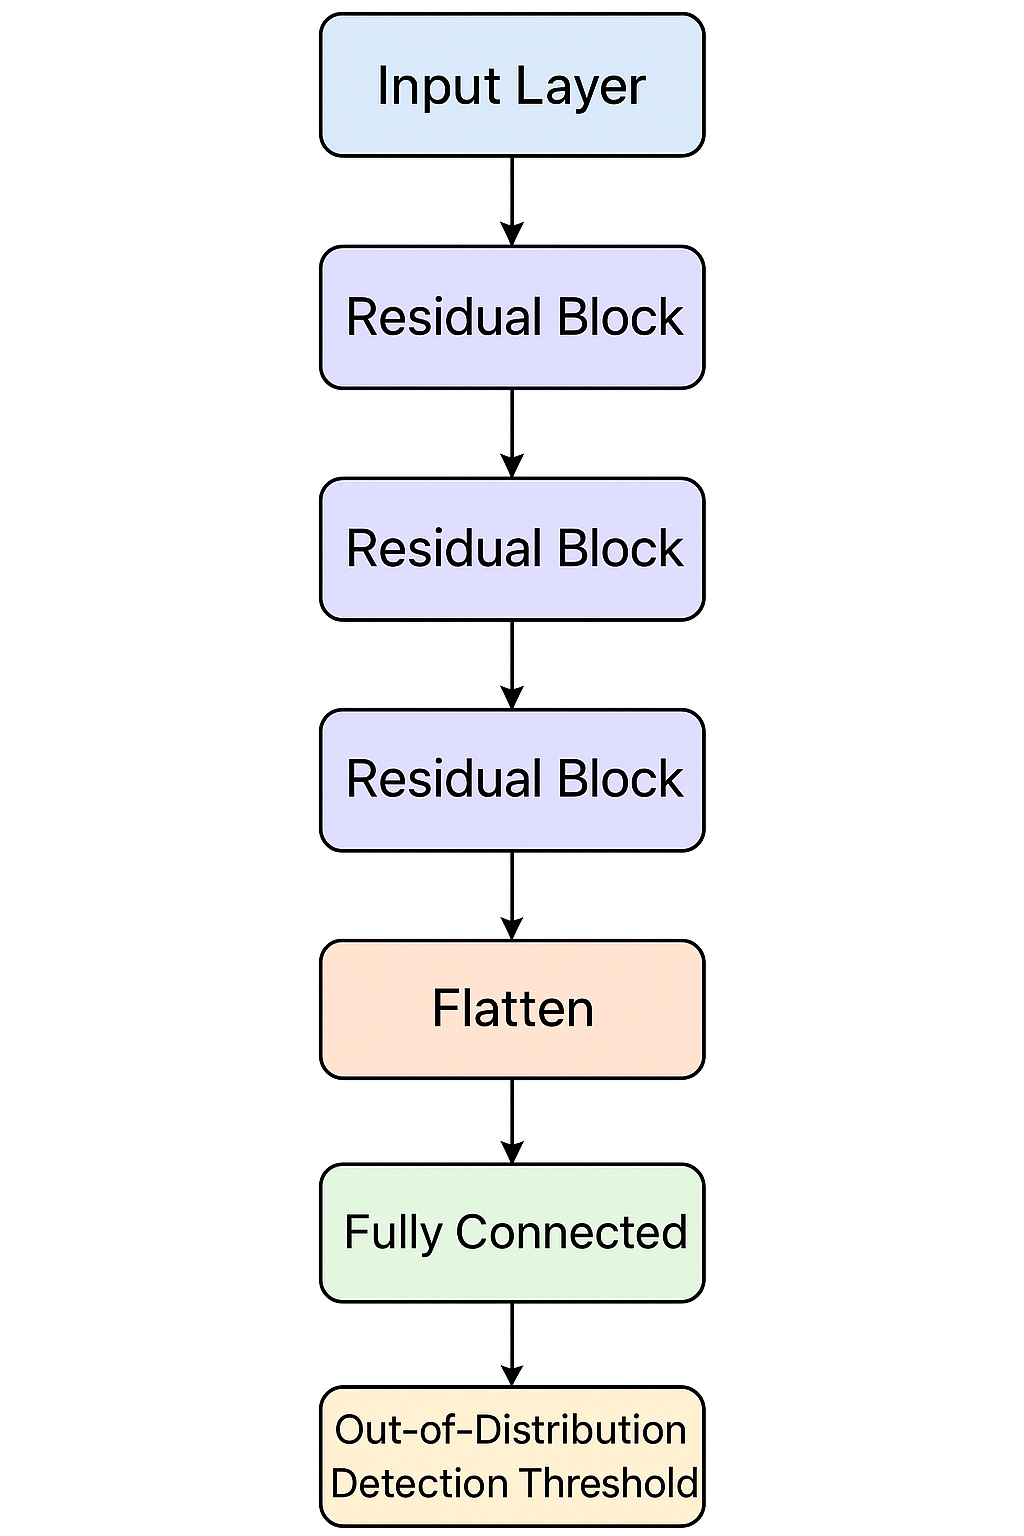
\includegraphics[width=0.5\linewidth]{cnn-architecture} 

}

\caption{CNN model Architecture for DermaAI}\label{fig:unnamed-chunk-16}
\end{figure}

\begin{itemize}
\tightlist
\item
  \textbf{Input Layer}: Accepts dermoscopic or non-dermoscopic images,
  resized and normalized to the required resolution.\\
\item
  \textbf{Feature Extraction (ResNet18 Backbone)}: Extracts hierarchical
  visual features such as edges, textures, and patterns, which are
  crucial for distinguishing between benign and malignant lesions.\\
\item
  \textbf{Fully Connected Layer}: Maps extracted features into class
  probabilities representing different categories of skin lesions (e.g.,
  melanoma, nevus, keratosis).\\
\item
  \textbf{Softmax Output}: Produces a probabilistic distribution,
  enabling ranking of likely conditions.\\
\item
  \textbf{Out-of-Distribution Handling}: Additional thresholds are set
  to identify and reject non-skin images or ambiguous inputs, reducing
  the risk of misdiagnosis.
\end{itemize}

The synergy between the \textbf{system-level serverless architecture}
and the \textbf{model-level CNN architecture} ensures both robust
backend scalability and high clinical relevance of predictions.

\subsection{User Interface Design}\label{user-interface-design}

The user interface (UI) design of the lesion detection system is
critical in ensuring usability, accessibility, and effective interaction
for different categories of end-users. Given the dual-interface
approach---mobile application for general users and command-line
interface (CLI) for health professionals and researchers---the system
emphasizes both simplicity and technical flexibility.

\subsubsection{Mobile Application
Interface}\label{mobile-application-interface}

The mobile application serves as the primary interaction point for
patients, general users, and non-technical healthcare providers. Its
design focuses on clarity, ease of use, and accessibility.

\paragraph{Input (Image Upload,
Metadata)}\label{input-image-upload-metadata}

Users can upload images of skin lesions captured through smartphone
cameras. To improve diagnostic accuracy, optional metadata such as age,
gender, and lesion location can also be provided. The app guides users
in capturing high-quality images through tips and validation prompts
(e.g., checking for blur or poor lighting).

\paragraph{Output (Prediction +
Explanation)}\label{output-prediction-explanation}

The app provides immediate feedback in the form of:

\begin{itemize}
\tightlist
\item
  \textbf{Prediction Results:} Displaying the likely classification of
  the skin lesion (e.g., melanoma, eczema, benign mole).\\
\item
  \textbf{Confidence Score:} A percentage value reflecting model
  certainty.\\
\item
  \textbf{AI-Generated Explanation:} Clear, user-friendly interpretation
  of the results, enhanced through integration with a Large Language
  Model (LLM) for contextual descriptions.
\end{itemize}

\paragraph{Additional Features (History, Notifications, Clinic
Suggestions)}\label{additional-features-history-notifications-clinic-suggestions}

\begin{itemize}
\tightlist
\item
  \textbf{History:} Users can view previously uploaded images and
  corresponding predictions.\\
\item
  \textbf{Notifications:} Timely alerts for follow-up checks, updates on
  results, or reminders to consult a specialist.\\
\item
  \textbf{Basic health information on lesions:} Provides updated
  information on common lesions
\end{itemize}

\subsubsection{Command-Line Interface
(CLI)}\label{command-line-interface-cli}

The CLI is designed for researchers, medical professionals, and advanced
users who require flexibility, scalability, and integration with
external workflows.

\paragraph{Input Methods (Single,
Batch)}\label{input-methods-single-batch}

\begin{itemize}
\tightlist
\item
  \textbf{Single Input:} Researchers can upload one image at a time for
  real-time classification.\\
\item
  \textbf{Batch Input:} The system supports batch processing of
  datasets, enabling large-scale testing and research.
\end{itemize}

\paragraph{Output Formats (CSV, JSON, PDF, Visual
Overlays)}\label{output-formats-csv-json-pdf-visual-overlays}

The CLI provides versatile output options, including:

\begin{itemize}
\tightlist
\item
  \textbf{CSV/JSON:} For structured data storage and integration with
  analytical pipelines.\\
\item
  \textbf{PDF Reports:} Automatically generated, summarizing results
  with statistics and visual representations.\\
\item
  \textbf{Visual Overlays:} Highlighting lesion areas directly on the
  images for deeper clinical inspection.
\end{itemize}

\subsection{Deployment Strategy}\label{deployment-strategy}

The deployment strategy for the lesion detection system balances
accessibility, scalability, and user needs. By leveraging cloud-native
services and serverless architecture, the system minimizes
infrastructure management while maximizing reliability and
cost-effectiveness.

\subsubsection{Cloud Deployment (Primary
Mode)}\label{cloud-deployment-primary-mode}

The system is primarily deployed on a cloud platform using a
\textbf{serverless architecture}. This approach ensures scalability and
efficient use of resources, as services such as AWS Lambda, Amazon S3,
and DynamoDB dynamically adjust to varying workloads. The cloud handles
the heavy computational tasks, including model inference and LLM-based
description generation. This guarantees high availability, data
security, and seamless integration of components without requiring users
to manage complex configurations.

\subsubsection{Command-Line Interface (CLI)
Deployment}\label{command-line-interface-cli-deployment}

For researchers and advanced users, the CLI tool serves as a flexible
deployment option. It connects directly to the cloud services for
inference, allowing single-image or batch processing. CLI deployment
supports structured outputs (CSV/JSON) and integrates easily with local
research environments.

A limited \textbf{offline mode} is available within the CLI:

\begin{itemize}
\tightlist
\item
  Offline capabilities do not include full model inference (to avoid
  heavy storage and computation requirements).\\
\item
  Instead, the offline mode provides \textbf{basic lesion information}
  (e.g., common types, risk factors, preventive measures), ensuring
  users have access to essential knowledge without requiring internet
  connectivity.
\end{itemize}

This offline functionality supports fieldwork and scenarios with
unstable connectivity, particularly useful for outreach programs and
rural healthcare settings.

\subsubsection{Mobile Application
Deployment}\label{mobile-application-deployment}

The mobile application is available for end-users through app
distribution platforms (Google Play Store, Apple App Store). Its
deployment strategy emphasizes accessibility and user-friendliness, with
real-time communication to the cloud backend for inference.

The \textbf{offline mode in the mobile app} is intentionally
lightweight:

\begin{itemize}
\tightlist
\item
  It does not include model inference, as shipping the CNN model locally
  would make the app too large and resource-heavy.\\
\item
  Instead, it provides an \textbf{offline reference guide}, featuring
  descriptions of common skin lesions, self-care recommendations, and
  educational material.\\
\item
  When online, the app automatically switches to full functionality,
  including image uploads, model inference, and enriched LLM
  explanations.
\end{itemize}

\begin{figure}

{\centering 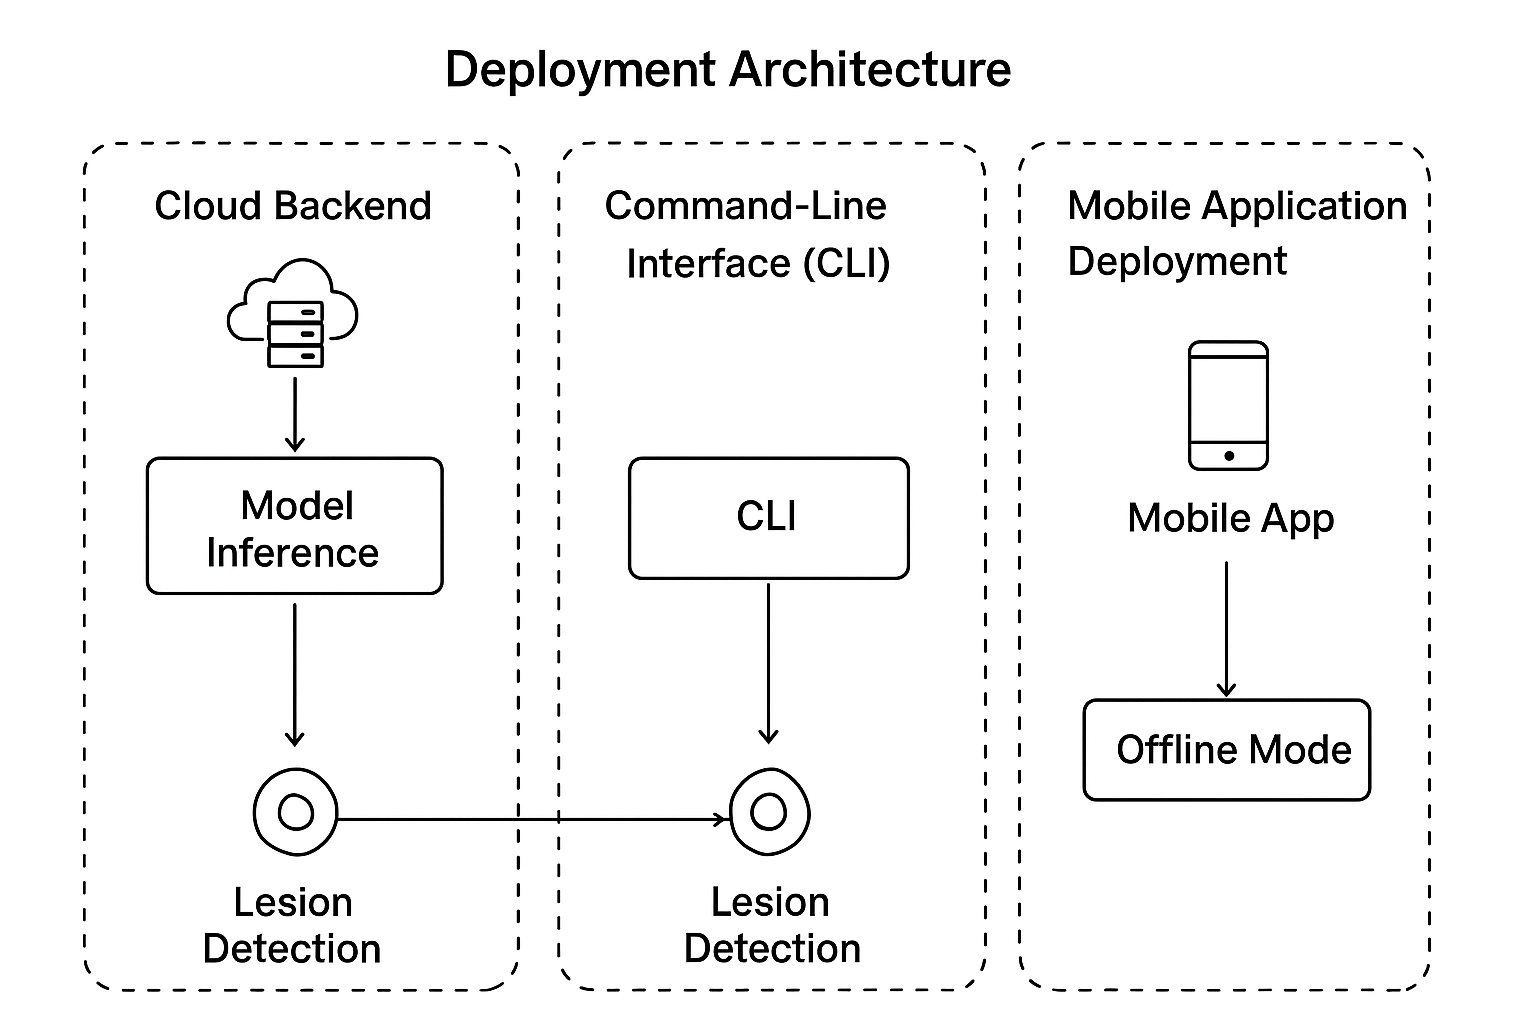
\includegraphics[width=0.7\linewidth]{deployement-architecture} 

}

\caption{Deployment Architecture for DermaAI}\label{fig:unnamed-chunk-17}
\end{figure}

\subsection{Testing, Results, and
Discussion}\label{testing-results-and-discussion}

\subsubsection{Dataset Splits (Train, Validation,
Test)}\label{dataset-splits-train-validation-test}

\subsubsection{Accuracy, Loss, and Confusion
Matrix}\label{accuracy-loss-and-confusion-matrix}

\subsubsection{ROC, Precision, Recall,
F1-score}\label{roc-precision-recall-f1-score}

\subsubsection{Model Limitations and Observed
Bias}\label{model-limitations-and-observed-bias}

\subsubsection{Comparison with Existing
Systems}\label{comparison-with-existing-systems}

\subsubsection{Summary}\label{summary-2}

\subsection{Summary}\label{summary-3}

\newpage

\section{Chapter 6: Conclusion and
Recommendations}\label{chapter-6-conclusion-and-recommendations}

\begin{itemize}
\tightlist
\item
  6.1 Summary of Findings
\item
  6.2 Conclusion
\item
  6.3 Contributions of the Study
\item
  6.4 Recommendations for Future Work
\item
  6.5 Final Remarks
\end{itemize}

\newpage

\section{Appendices}\label{appendices}

\begin{itemize}
\tightlist
\item
  Appendix A: Source Code Snippets
\item
  Appendix B: Model Configurations
\item
  Appendix C: Training Graphs
\item
  Appendix D: Screenshots of GUI
\item
  Appendix E: User Manual
\end{itemize}

\newpage

\section*{References}\label{references}
\addcontentsline{toc}{section}{References}

\phantomsection\label{refs}
\begin{CSLReferences}{1}{0}
\bibitem[\citeproctext]{ref-adam2014method}
Adam, K. D. B. J. et al. (2014). A method for stochastic optimization.
\emph{arXiv Preprint arXiv:1412.6980}, \emph{1412}(6).

\bibitem[\citeproctext]{ref-adegun2020fcn}
Adegun, A. A., \& Viriri, S. (2020). FCN-based DenseNet framework for
automated detection and classification of skin lesions in dermoscopy
images. \emph{IEEE Access}, \emph{8}, 150377--150396.

\bibitem[\citeproctext]{ref-albahar2019skin}
Albahar, M. A. (2019). Skin lesion classification using convolutional
neural network with novel regularizer. \emph{IEEE Access}, \emph{7},
38306--38313.

\bibitem[\citeproctext]{ref-braun2006using}
Braun, V., \& Clarke, V. (2006). Using thematic analysis in psychology.
\emph{Qualitative Research in Psychology}, \emph{3}(2), 77--101.
\url{https://doi.org/10.1191/1478088706qp063oa}

\bibitem[\citeproctext]{ref-buda2018systematic}
Buda, M., Maki, A., \& Mazurowski, M. A. (2018). A systematic study of
the class imbalance problem in convolutional neural networks.
\emph{Neural Networks}, \emph{106}, 249--259.

\bibitem[\citeproctext]{ref-doshi2017towards}
Doshi-Velez, F., \& Kim, B. (2017). Towards a rigorous science of
interpretable machine learning. \emph{arXiv Preprint arXiv:1702.08608}.

\bibitem[\citeproctext]{ref-esteva2017dermatologist}
Esteva, A., Kuprel, B., Novoa, R. A., Ko, J., Swetter, S. M., Blau, H.
M., \& Thrun, S. (2017). Dermatologist-level classification of skin
cancer with deep neural networks. \emph{Nature}, \emph{542}(7639),
115--118.

\bibitem[\citeproctext]{ref-goodfellow2016deep}
Goodfellow, I., Bengio, Y., \& Courville, A. (2016). \emph{Deep
learning}. MIT Press. \url{https://www.deeplearningbook.org/}

\bibitem[\citeproctext]{ref-gouda2022detection}
Gouda, W., Sama, N. U., Al-Waakid, G., Humayun, M., \& Jhanjhi, N. Z.
(2022). Detection of skin cancer based on skin lesion images using deep
learning. \emph{Healthcare}, \emph{10}, 1183.

\bibitem[\citeproctext]{ref-haenssle2018man}
Haenssle, H. A., Fink, C., Schneiderbauer, R., Toberer, F., Bäuerle, A.,
Blum, A., Kalloo, A., Hassen, A. B. H., Thomas, L., Enk, A., Uhlmann,
L., \& Reader study group, M. against machine. (2018). Man against
machine: Diagnostic performance of a deep learning convolutional neural
network for dermoscopic melanoma recognition in comparison to 58
dermatologists. \emph{Annals of Oncology}, \emph{29}(8), 1836--1842.

\bibitem[\citeproctext]{ref-harangi2018skin}
Harangi, B. (2018). Skin lesion classification with ensembles of deep
convolutional neural networks. \emph{Journal of Biomedical Informatics},
\emph{86}, 25--32.

\bibitem[\citeproctext]{ref-hay2006skin}
Hay, R., Bendeck, S. E., Chen, S., Estrada, R., Haddix, A., McLeod, T.,
\& Mahé, A. (2006). Skin diseases. \emph{Disease Control Priorities in
Developing Countries. 2nd Edition}.

\bibitem[\citeproctext]{ref-he2016deep}
He, K., Zhang, X., Ren, S., \& Sun, J. (2016). Deep residual learning
for image recognition. \emph{Proceedings of the IEEE Conference on
Computer Vision and Pattern Recognition}, 770--778.

\bibitem[\citeproctext]{ref-van2005common}
Hees, C. van, \& Naafs, B. (2005). \emph{Common skin diseases africa}.

\bibitem[\citeproctext]{ref-holzinger2017we}
Holzinger, A., Biemann, C., Pattichis, C. S., \& Kell, D. B. (2017).
What do we need to build explainable AI systems for the medical domain?
In \emph{Machine learning and knowledge extraction} (pp. 1--28).
Springer.

\bibitem[\citeproctext]{ref-jinnai2020development}
Jinnai, S., Yamazaki, N., Hirano, Y., Sugawara, Y., Ohe, Y., \&
Hamamoto, R. (2020). The development of a skin cancer classification
system for pigmented skin lesions using deep learning.
\emph{Biomolecules}, \emph{10}(8), 1123.

\bibitem[\citeproctext]{ref-kassem2021machine}
Kassem, M. A., Hosny, K. M., Damaševičius, R., \& Eltoukhy, M. M.
(2021). Machine learning and deep learning methods for skin lesion
classification and diagnosis: A systematic review. \emph{Diagnostics},
\emph{11}(8), 1390.

\bibitem[\citeproctext]{ref-khan2021multi}
Khan, M. A., Muhammad, K., Sharif, M., Akram, T., \& Albuquerque, V. H.
C. de. (2021). Multi-class skin lesion detection and classification via
teledermatology. \emph{IEEE Journal of Biomedical and Health
Informatics}, \emph{25}(12), 4267--4275.

\bibitem[\citeproctext]{ref-krawczyk2016learning}
Krawczyk, B. (2016). Learning from imbalanced data: Open challenges and
future directions. \emph{Progress in Artificial Intelligence},
\emph{5}(4), 221--232. \url{https://doi.org/10.1007/s13748-016-0094-0}

\bibitem[\citeproctext]{ref-lecun2015deep}
LeCun, Y., Bengio, Y., \& Hinton, G. (2015). Deep learning.
\emph{Nature}, \emph{521}(7553), 436--444.

\bibitem[\citeproctext]{ref-mahbod2019skin}
Mahbod, A., Schaefer, G., Wang, C., Ecker, R., \& Ellinge, I. (2019).
Skin lesion classification using hybrid deep neural networks.
\emph{ICASSP 2019-2019 IEEE International Conference on Acoustics,
Speech and Signal Processing (ICASSP)}, 1229--1233.

\bibitem[\citeproctext]{ref-ogudo2023optimal}
Ogudo, K. A., Surendran, R., \& Khalaf, O. I. (2023). Optimal artificial
intelligence based automated skin lesion detection and classification
model. \emph{Computer Systems Science \& Engineering}, \emph{44}(1).

\bibitem[\citeproctext]{ref-prechelt1998early}
Prechelt, L. (1998). Early stopping---but when? \emph{Neural Networks:
Tricks of the Trade}, 55--69.
\url{https://doi.org/10.1007/3-540-49430-8_3}

\bibitem[\citeproctext]{ref-ruparelia2010software}
Ruparelia, N. B. (2010). Software development lifecycle models.
\emph{ACM SIGSOFT Software Engineering Notes}, \emph{35}(3), 8--13.

\bibitem[\citeproctext]{ref-shafiq2021literature}
Shafiq, S., Mashkoor, A., Mayr-Dorn, C., \& Egyed, A. (2021). A
literature review of using machine learning in software development life
cycle stages. \emph{IEEe Access}, \emph{9}, 140896--140920.

\bibitem[\citeproctext]{ref-srivastava2017scrum}
Srivastava, A., Bhardwaj, S., \& Saraswat, S. (2017). SCRUM model for
agile methodology. \emph{2017 International Conference on Computing,
Communication and Automation (ICCCA)}, 864--869.

\bibitem[\citeproctext]{ref-tschandl2018ham10000}
Tschandl, P., Rosendahl, C., \& Kittler, H. (2018). The HAM10000
dataset, a large collection of multi-source dermatoscopic images of
common pigmented skin lesions. \emph{Scientific Data}, \emph{5}(1),
1--9.

\bibitem[\citeproctext]{ref-ventola2014mobile}
Ventola, C. L. (2014). Mobile devices and apps for health care
professionals: Uses and benefits. \emph{P \& T: A Peer-Reviewed Journal
for Formulary Management}, \emph{39}(5), 356--364.

\bibitem[\citeproctext]{ref-yap2018multimodal}
Yap, J., Yolland, W., \& Tschandl, P. (2018). Multimodal skin lesion
classification using deep learning. \emph{Experimental Dermatology},
\emph{27}(11), 1261--1267.

\bibitem[\citeproctext]{ref-yosinski2014transfer}
Yosinski, J., Clune, J., Bengio, Y., \& Lipson, H. (2014). How
transferable are features in deep neural networks? \emph{Advances in
Neural Information Processing Systems}, \emph{27}.

\bibitem[\citeproctext]{ref-zafar2023skin}
Zafar, M., Sharif, M. I., Sharif, M. I., Kadry, S., Bukhari, S. A. C.,
\& Rauf, H. T. (2023). Skin lesion analysis and cancer detection based
on machine/deep learning techniques: A comprehensive survey.
\emph{Life}, \emph{13}(1), 146.

\end{CSLReferences}

\end{document}
